% Options for packages loaded elsewhere
\PassOptionsToPackage{unicode}{hyperref}
\PassOptionsToPackage{hyphens}{url}
\PassOptionsToPackage{dvipsnames,svgnames,x11names}{xcolor}
%
\documentclass[
  letterpaper,
  DIV=11,
  numbers=noendperiod]{scrartcl}

\usepackage{amsmath,amssymb}
\usepackage{iftex}
\ifPDFTeX
  \usepackage[T1]{fontenc}
  \usepackage[utf8]{inputenc}
  \usepackage{textcomp} % provide euro and other symbols
\else % if luatex or xetex
  \usepackage{unicode-math}
  \defaultfontfeatures{Scale=MatchLowercase}
  \defaultfontfeatures[\rmfamily]{Ligatures=TeX,Scale=1}
\fi
\usepackage{lmodern}
\ifPDFTeX\else  
    % xetex/luatex font selection
\fi
% Use upquote if available, for straight quotes in verbatim environments
\IfFileExists{upquote.sty}{\usepackage{upquote}}{}
\IfFileExists{microtype.sty}{% use microtype if available
  \usepackage[]{microtype}
  \UseMicrotypeSet[protrusion]{basicmath} % disable protrusion for tt fonts
}{}
\makeatletter
\@ifundefined{KOMAClassName}{% if non-KOMA class
  \IfFileExists{parskip.sty}{%
    \usepackage{parskip}
  }{% else
    \setlength{\parindent}{0pt}
    \setlength{\parskip}{6pt plus 2pt minus 1pt}}
}{% if KOMA class
  \KOMAoptions{parskip=half}}
\makeatother
\usepackage{xcolor}
\setlength{\emergencystretch}{3em} % prevent overfull lines
\setcounter{secnumdepth}{5}
% Make \paragraph and \subparagraph free-standing
\ifx\paragraph\undefined\else
  \let\oldparagraph\paragraph
  \renewcommand{\paragraph}[1]{\oldparagraph{#1}\mbox{}}
\fi
\ifx\subparagraph\undefined\else
  \let\oldsubparagraph\subparagraph
  \renewcommand{\subparagraph}[1]{\oldsubparagraph{#1}\mbox{}}
\fi


\providecommand{\tightlist}{%
  \setlength{\itemsep}{0pt}\setlength{\parskip}{0pt}}\usepackage{longtable,booktabs,array}
\usepackage{calc} % for calculating minipage widths
% Correct order of tables after \paragraph or \subparagraph
\usepackage{etoolbox}
\makeatletter
\patchcmd\longtable{\par}{\if@noskipsec\mbox{}\fi\par}{}{}
\makeatother
% Allow footnotes in longtable head/foot
\IfFileExists{footnotehyper.sty}{\usepackage{footnotehyper}}{\usepackage{footnote}}
\makesavenoteenv{longtable}
\usepackage{graphicx}
\makeatletter
\def\maxwidth{\ifdim\Gin@nat@width>\linewidth\linewidth\else\Gin@nat@width\fi}
\def\maxheight{\ifdim\Gin@nat@height>\textheight\textheight\else\Gin@nat@height\fi}
\makeatother
% Scale images if necessary, so that they will not overflow the page
% margins by default, and it is still possible to overwrite the defaults
% using explicit options in \includegraphics[width, height, ...]{}
\setkeys{Gin}{width=\maxwidth,height=\maxheight,keepaspectratio}
% Set default figure placement to htbp
\makeatletter
\def\fps@figure{htbp}
\makeatother
\newlength{\cslhangindent}
\setlength{\cslhangindent}{1.5em}
\newlength{\csllabelwidth}
\setlength{\csllabelwidth}{3em}
\newlength{\cslentryspacingunit} % times entry-spacing
\setlength{\cslentryspacingunit}{\parskip}
\newenvironment{CSLReferences}[2] % #1 hanging-ident, #2 entry spacing
 {% don't indent paragraphs
  \setlength{\parindent}{0pt}
  % turn on hanging indent if param 1 is 1
  \ifodd #1
  \let\oldpar\par
  \def\par{\hangindent=\cslhangindent\oldpar}
  \fi
  % set entry spacing
  \setlength{\parskip}{#2\cslentryspacingunit}
 }%
 {}
\usepackage{calc}
\newcommand{\CSLBlock}[1]{#1\hfill\break}
\newcommand{\CSLLeftMargin}[1]{\parbox[t]{\csllabelwidth}{#1}}
\newcommand{\CSLRightInline}[1]{\parbox[t]{\linewidth - \csllabelwidth}{#1}\break}
\newcommand{\CSLIndent}[1]{\hspace{\cslhangindent}#1}

\usepackage{booktabs}
\usepackage{longtable}
\usepackage{array}
\usepackage{multirow}
\usepackage{wrapfig}
\usepackage{float}
\usepackage{colortbl}
\usepackage{pdflscape}
\usepackage{tabu}
\usepackage{threeparttable}
\usepackage{threeparttablex}
\usepackage[normalem]{ulem}
\usepackage{makecell}
\usepackage{xcolor}
\usepackage{booktabs}
\usepackage{siunitx}
\usepackage{multirow}
\newcommand{\beginsupplement}{\setcounter{section}{0} \renewcommand{\thesection}{A\arabic{section}}  \setcounter{table}{0}  \renewcommand{\thetable}{A\arabic{table}} \setcounter{figure}{0} \renewcommand{\thefigure}{A\arabic{figure}}}
\KOMAoption{captions}{tableheading,figureheading}
\makeatletter
\makeatother
\makeatletter
\makeatother
\makeatletter
\@ifpackageloaded{caption}{}{\usepackage{caption}}
\AtBeginDocument{%
\ifdefined\contentsname
  \renewcommand*\contentsname{Table of contents}
\else
  \newcommand\contentsname{Table of contents}
\fi
\ifdefined\listfigurename
  \renewcommand*\listfigurename{List of Figures}
\else
  \newcommand\listfigurename{List of Figures}
\fi
\ifdefined\listtablename
  \renewcommand*\listtablename{List of Tables}
\else
  \newcommand\listtablename{List of Tables}
\fi
\ifdefined\figurename
  \renewcommand*\figurename{Figure}
\else
  \newcommand\figurename{Figure}
\fi
\ifdefined\tablename
  \renewcommand*\tablename{Table}
\else
  \newcommand\tablename{Table}
\fi
}
\@ifpackageloaded{float}{}{\usepackage{float}}
\floatstyle{ruled}
\@ifundefined{c@chapter}{\newfloat{codelisting}{h}{lop}}{\newfloat{codelisting}{h}{lop}[chapter]}
\floatname{codelisting}{Listing}
\newcommand*\listoflistings{\listof{codelisting}{List of Listings}}
\makeatother
\makeatletter
\@ifpackageloaded{caption}{}{\usepackage{caption}}
\@ifpackageloaded{subcaption}{}{\usepackage{subcaption}}
\makeatother
\makeatletter
\@ifpackageloaded{tcolorbox}{}{\usepackage[skins,breakable]{tcolorbox}}
\makeatother
\makeatletter
\@ifundefined{shadecolor}{\definecolor{shadecolor}{rgb}{.97, .97, .97}}
\makeatother
\makeatletter
\makeatother
\makeatletter
\makeatother
\ifLuaTeX
  \usepackage{selnolig}  % disable illegal ligatures
\fi
\IfFileExists{bookmark.sty}{\usepackage{bookmark}}{\usepackage{hyperref}}
\IfFileExists{xurl.sty}{\usepackage{xurl}}{} % add URL line breaks if available
\urlstyle{same} % disable monospaced font for URLs
\hypersetup{
  pdftitle={Can we predict multi-party elections with Google Trends data? Evidence across elections, data windows, and model classes},
  pdfauthor={Jan Behnert; Dean Lajic; Paul C. Bauer},
  pdfkeywords={Google Trends, Election, Prediction},
  colorlinks=true,
  linkcolor={blue},
  filecolor={Maroon},
  citecolor={Blue},
  urlcolor={Blue},
  pdfcreator={LaTeX via pandoc}}

\title{Can we predict multi-party elections with Google Trends data?
Evidence across elections, data windows, and model classes}
\author{Jan Behnert \and Dean Lajic \and Paul C. Bauer}
\date{2023-06-12}

\begin{document}
\maketitle
\begin{abstract}
Google trends (GT), a service aggregating search queries on Google, has
been used to predict various outcomes such as as the spread of
influenza, automobile sales, unemployment claims, and travel destination
planning (1,2). Social scientists also used GT to predict elections and
referendums across different countries and time periods, sometimes with
more, sometimes with less success. We provide unique evidence on the
predictive power of GT in the German multi-party systems, forecasting
four elections (2009, 2013, 2017, 2021). Thereby, we make several
contributions: First, we present one of the first attempts to predict a
multi-party election using GT and highlight the specific challenges that
originate from this setting. In doing so, we also provide a
comprehensive and systematic overview of prior research. Second, we
develop a framework that allows for fine-grained variation of the GT
data window both in terms of its width and distance to the election.
Subsequently, we test the predictive accuracy of several thousand models
resulting from those fine-grained specifications. Third, we compare the
predictive power of different model classes that are purely GT data
based but also incorporate polling data as well as previous elections.
Finally, we provide a systematic overview of the challenges one faces in
using GT data for predictions part of which have been neglected in prior
research.
\end{abstract}
\ifdefined\Shaded\renewenvironment{Shaded}{\begin{tcolorbox}[enhanced, frame hidden, sharp corners, boxrule=0pt, borderline west={3pt}{0pt}{shadecolor}, interior hidden, breakable]}{\end{tcolorbox}}\fi

\renewcommand*\contentsname{Table of contents}
{
\hypersetup{linkcolor=}
\setcounter{tocdepth}{3}
\tableofcontents
}
\newpage

\hypertarget{introduction}{%
\section{Introduction}\label{introduction}}

Google trends (GT), a service aggregating search queries on Google, has
been used to predict various outcomes such as the spread of influenza,
automobile sales, unemployment claims, and travel destination planning
(2). These sparked the interest of political scientists who subsequently
used GT data to predict elections with binary outcomes, e.g.,
presidential elections in the US or referenda such as the Brexit
referendum, and, often claim to be successful (7). In principle, Google
Trends could provide a cheap data source that may extend previous
predictive models that rely on polling data as well as structural data
such as previous election results (10). Exploring new data sources such
as GT is also warranted given the persisting discussion on the validity
of polling data (13).\footnote{More recently, scholars have turned to
  using reweighted non-representative polls to predict elections (e.g.,
  13).}\\
In our study we pursue the following research question: Can we use
Google Trends data to predict election results in a multi-party system?
Thereby, we make a series of contributions to scholarship using GT for
predictive purposes generally but also specifically for elections:
First, we are among the first to evidence on the predictive power of GT
in the multi-party system setting. Thereby, we use GT to predict four
elections in Germany and highlight the specific challenges that
originate from the multi-party context. We also provide a systematic
review of previous research highlighting variation across several
important dimensions. This review both helps us to highlight our
contributions and can represent a starting point for future research on
GT predictions (see Table~\ref{tbl-2}).\\
Second, when using GT for predictions one of the most important choices
lies in the GT data window on which those predictions are based. The
data window may vary in terms of width, e.g., our prediction could be
based on averaging 1 week of GT data as opposed to 3 weeks of GT data.
And, the data window may vary in terms of distance to the event that
shall be predicted, e.g., we could predict an election using a data
window that ends just two days before the election or a data window that
ends three months before the election. Granka (14) suggested to explore
moving averages to assess how well models withstand changes closer to
the election date. While previous studies have varied these aspects, we
are the first to build a framework that allows to cycle through
fine-grained values of both width and distance testing the predictive
accuracy of thousands of resulting models.\\
Third, following previous studies, we compare the predictive power of
different model classes. Besides, a model that only includes GT data, we
explore the predictive accuracy of models that combine GT data with
election data and polling data. And, we compare our predictions to
simple polling data. This provides us with an answer as to whether GT
really does represent an alternative to classic purely poll-based
methods and whether combinations are fruitful.\\
Fourth, we provide a systematic overview of the challenges one faces in
using GT data for predictions part of which have been neglected in prior
research. These comprise choices on the GT platform, e.g., we can
restrict that data to searches belonging to certain categories, but also
the varying nature of GT data across samples. We discuss which previous
studies have acknowledged these and other challenges and tackle them in
a systematic fashion to study their impact. Thereby, we provide a
blueprint for future GT research.\\
In Section~\ref{sec-review} we start by providing an overview of
research that leverages GT data for predictive purposes generally but
also for political outcomes. In Section~\ref{sec-methodology} we explain
our methodological approach, the data we are collecting and using as
well as the predictive models we are building. Section~\ref{sec-results}
presents our results namely the predictions of four elections. In the
conclusion we summarize the most important insights (see
Section~\ref{sec-conclusion}).

\hypertarget{sec-review}{%
\section{Using Google Trends to predict elections and other
phenomena}\label{sec-review}}

The proportion of internet users aged 14 and over in Germany has risen
from 37\% in 1991 to 91\% individuals aged 14 and older (15). In terms
of search engines Google is by far the dominant search engine with
market shares of 80.4\% (desktop) and 96.8\% (mobile) (16). Nonetheless,
as we will discuss below, Google users are not necessarily
representative of the German electorate.

\hypertarget{predicting-phenomena-with-google-trends}{%
\subsection{Predicting phenomena with Google
Trends}\label{predicting-phenomena-with-google-trends}}

Google has made its data on Google searches freely available for
everyone in the year 2006 (see https://trends.google.com/). Rather than
absolute numbers of searches, GT provides data on interest in a search
term relative to all other search terms in a country or region over a
selected period of time. GT data comes along with certain advantages
such as cost-free access to aggregated big data, a sample that is
(ideally) representative of all Google searches or an unfiltered
real-time sample. Soon after going public GT made headlines and the
number of studies using GT data has grown significantly. In general, the
assumption underlying those studies is that search queries in Google
reflect the genuine interests or intentions of people. While GT was most
frequently used in the field of Computer Science, usage in other
disciplines has picked up (17). In a ground-breaking study Ginsberg and
colleagues used GT data and its real-time nature to predict the spread
of influenza, comparing its accuracy to predictions by the Government
Agency Center for Disease Control and Prevention (CDC) (2). This first
study started a debate on the advantages but also deficiencies of GT flu
predictions (20). The enormous potential of GT data was also
demonstrated by Choi \& Varian (1), who predicted economic indicators
including automobile sales, unemployment claims, travel destination
planning, etc. The continued popularity is reflected in recently
published papers that used GT data in the context of the COVID-19
pandemic. Brodeur et al. (21) for example examined whether COVID-19 and
the associated lockdowns initiated in Europe and America led to changes
in well-being.

\hypertarget{predicting-elections-with-google-trends}{%
\subsection{Predicting elections with Google
Trends}\label{predicting-elections-with-google-trends}}

Table~\ref{tbl-1} summarizes studies that have used GT data to predict
elections. Reviewing the literature a few aspects stand out. First, the
focus usually lies on binary electoral outcomes. Prado-Román et al. (7),
for example, were able to predict the final results of all presidential
elections in the US and Canada for the time period 2004 -- 2016.
Polykalas et al. (22) were able to forecast Greek and Spain election
results. However, other studies found GT to be less helpful in
predicting elections, despite their focus on binary settings (24). Other
studies illustrated that GT data can be used to predict referendum
results {[}(3), (4)). (6) successfully predicted six referendums in
different countries in Europe between 2014 and 2016, for example the
Brexit referendum. Polykalas et al. (25) used GT to predict elections in
Germany, examining only the two most popular parties, the SPD and the
CDU, trying to predict which of the two parties will win. In contrast to
the previously mentioned studies, the authors additionally weight their
GT predictions using previous election results to control for the
selection bias, i.e., the fact that not everyone uses the internet. As
indicated in Table~\ref{tbl-1}, one of the few exceptions predicting
multi-party elections is (26). Sjövill's thesis uses GT data to predict
party shares focusing on the three Swedish federal elections 2010, 2014
and 2018. Sjövill (26) emphasizes the importance of weighting the GT
predictions using previous final election results and polling data, to
control for the sample selection bias of GT data. Sjövill (26) compares
different models with the different weighting methods and finds that they
mostly have the same predictive accuracy as the average of pre-election
opinion polls. The weighting method using actual polling data proved to
be the most informative. Second, the GT data window that is used for the
prediction is defined through its width, i.e., the end time minus the
start time of the window, and the distance to the event that shall be
predicted. Across studies there is strong variation in terms of the GT
data windows chosen both in terms of width and distance (cf.
Table~\ref{tbl-1}). Most studies pick one to three different widths,
usually one week or one month. And, in terms of distance studies usually
pick a data window that ends just before the election. Naturally, the
question arises whether the findings made across these studies would be
the same if we were to vary the width and distance of the underlying GT
data. It is one of our aims to provide a more systematic approach to
choosing the data window comparing predictions for a wide variety of
choices. Third, while researchers have compared GT predictions to
classical polling data, they have also explored different weighting
schemes that may decrease sample selection bias (26). Sample selection
bias is present if, e.g., voters of conservative parties are on average
older and thus use the internet less. As a consequence they are
underrepresented among Google users leading to an underestimation of the
vote share of conservative parties. Polykalas et al. (25) weighted their
GT predictions with election results from the previous election. Sjövill
(26) constructed three different models: A long-term model that weighs
GT predictions with partys' previous election results; an intermediate
model weighting the GT predictions using semi-annual and highly
representative polling data from a respected election poll in Sweden;
and a short-term model which used average monthly polling data for
weighting. While all models came close to the results of the election
polls in the election years studied, the short time model proved to be
the most informative. Inspired by this research we also compare
different weighting schemes as described in Section~\ref{sec-models}.
Finally, with few exceptions, most studies remain silent on a set of
important characteristics of the GT platform and its data. At the same
time these characteristics can affect any predictive exercise. A first
issue is that data provided by GT represents a random sample that
changes over time (27). As summarized in Table~\ref{tbl-1}, column
``Multiple GT datasets'', we only found one study that bases its
predictions on several GT data samples (27). Following Raubenheimer et
al. (27) we develop a systematic sampling strategy for GT data and
average our predictions across those samples as described in
Section~\ref{sec-gtdatacollection} and Section~\ref{sec-gtsampling}. A
second issue is the selection of GT search terms (see
Section~\ref{sec-searchterms}). This selection potentially has the
strongest effect on any predictions we make, hence, transparently
communicating how and following which rational these terms have been
selected is of utmost importance. A third issue is whether to further
refine search terms by picking a category filter provided by Google (see
Section~\ref{sec-categoryfilter}). Such filters attempt to identify
searches that belong to particular topics helping to identify only
relevant searches. With the exception of Mavragani \& Tsagarakis (6) no
previous studies made use of such categories filters (cf.~column ``Cat.
used'' in Table~\ref{tbl-1}). Below, we compare the impact of basing
predictions on searches refined through such a category and non-refined
searches.

\hypertarget{tbl-1}{}
\begin{table}
\caption{\label{tbl-1}Overview of choices in previous studies }\tabularnewline

\centering\begingroup\fontsize{6}{8}\selectfont

\begin{tabular}{>{\raggedright\arraybackslash}p{0.8in}>{\raggedright\arraybackslash}p{1in}>{\raggedright\arraybackslash}p{0.4in}>{\raggedright\arraybackslash}p{0.6in}>{\raggedright\arraybackslash}p{0.4in}>{\raggedright\arraybackslash}p{0.4in}>{\raggedright\arraybackslash}p{0.3in}>{\raggedright\arraybackslash}p{0.3in}}
\toprule
Study & Election(s) & Width(s) & Dist. & Cat. used & Data type used & Multiple GT datasets & Explain / mention search term selection\\
\midrule
Peer-reviewed &  &  &  &  &  &  & \\
Raubenheimer et al. (2021) & 2020 New Zealand cannabis referendum & 1 week; 3 months & N = 1; 1 day before event & no & hourly daily & yes & yes\\
Prado-Román et al. (2021) & 2004-2016 presidential elections US \& 2004-2019 presidential elections Canada & 1/2/3 month(s) & N = 1; 1 day before event & ? & daily & no & no\\
Mavragani et al. (2019) & The 2014 Scottish the 2015 Greek the 2016 UK Hungarian Italian and the 2017 Turkish Referendum & 1 week; 1 month & N = 1; 1 day before event & yes (no further explanation why) & hourly daily & no & no\\
Mavragani \& Tsagarakis (2016) & Greek referendum 2015 & 8 days; 1 day; 12 hours & N = 1; 1 day before event \& N= 0; on Referendum day & ? & hourly & no & yes\\
\addlinespace
Polykalas et al. (2013a) & 2005-2013 German Elections (only parties CDU/SPD) & 1 month & N = 1; 1 day before event & ? & daily & no & yes\\
Harkan \& Eryanto (2021) & 2019 Indonesian Presidential Election & 23. Sept 2018- 16 May 2019 & N = 1; 1 day before event & no & weekly? & no & no\\
Polykalas et al. (2013b) & Greek elections 2007-2012 \& Spanish national elections 2008-2011 & 1 month & 1 day; 1/2 week(s) & ? & daily & no & yes\\
Yasseri \& Bright (2013) & Iranian election 2013 German election 2013 UK election 2010 & ? & ? & ? & daily? & no & no\\
Granka (2013) & US Presidential Elections 4' 8' and 12' & 1 month & 2 months & no & weekly & no & no\\
\addlinespace
Vergara-Perucich (2022) & Chile: Presidential election 2006--2021 & 121 days & 5 days & ? & daily & no & no\\
 &  &  &  &  &  &  & \\
Non-peer reviewed &  &  &  &  &  &  & \\
Sjövill (2020)* & Swedish general election 2010-2018 & 1/2 weeks; 1 month & N = 1; 1 day before event & no & daily & no & yes\\
Wolf (2018) & US Presidential Elections 16' swing states & 2/4 days & Depending on poll data & no & daily hourly? & no & ?\\
\addlinespace
Askitas (2015b) & Greek referendum 2015 & 1 week & N = 1; 1 day before event & no & hourly & no & yes\\
Askitas (2015a) & Irish "Gay Marriage" Referendum 2015 & 1 week & N = 1; 1 day before event & no & hourly & no & yes\\
\bottomrule
\multicolumn{8}{l}{\rule{0pt}{1em}\textit{Note: }}\\
\multicolumn{8}{l}{\rule{0pt}{1em}* = Non-binary outcome; ? = not enough information}\\
\end{tabular}
\endgroup{}
\end{table}

\hypertarget{sec-methodology}{%
\section{Data and Method}\label{sec-methodology}}

In our analysis we rely on three types of data, Google trends data (see
Section~\ref{sec-gtdatacollection}) as well as data on polls and actual
election results (see Section~\ref{sec-polldatacollection}).

\hypertarget{sec-gtdata}{%
\subsection{Google Trends as a data source}\label{sec-gtdata}}

GT provides access to a largely unfiltered sample of ``real-time''
searches on different topics (up to 36h before the actual time you
conduct the search) or a filtered and representative sample (as claimed
by Google) of searches that are older than 36 hours starting from the
year 2004. The data can be obtained for different search types that
correspond to different Google products like ``Web search,'' ``News,''
``Images,'' ``Shopping'' and ``Youtube''. Importantly, GT does not
provide access to data on individual searches. Rather the data is
anonymized and Google aggregates the data to the federal state level,
country level or world level. Besides, it is possible to filter searches
belonging to different categories, e.g., ``Law and Government'', with
the aim of only getting searches for the word's meaning one is
interested in. The result we get are a standardized, relative measure of
search volume for a single word/search term, a combination of search
terms using operators,\footnote{Available Operators: No quotation marks
  (results for each word in your query), Quotation marks (coherent
  search phrase), Plus sign (serves as function of an OR-operator) and
  Minus sign (Excludes word after the operator) \textbf{(Google Trends
  Help 2023d)}.} or comparisons, i.e., one input in relation to the
other inputs,\footnote{Possible to compare up to five groups of terms at
  one time and up to 25 terms in each group (Google Trends Help 2023a).}
over a selected time period. Google calculates how much search volume in
each region a search term or query had, relative to all searches in that
region. Using this information, Google assigns a measure of popularity
to search terms (scale of 0 - 100), leaving out repeated searches from
the same person over a short period of time and searches with
apostrophes and other special characters (28). The maximum of the scale
corresponds to a search term's maximum level of popularity relative to
other search terms and time periods.

\hypertarget{sec-searchterms}{%
\subsection{Search terms and category filter}\label{sec-searchterms}}

The first step in using Google searches to predict phenomena is the
selection of search terms on which we base our predictions. Since words
may have multiple meanings, e.g., jaguar could be an animal or a car, GT
provides a category filter to get data for the right version of the
word. Only one previous study made use of the category filter in Google
Trends (6), a shortcoming since categories help purge the search term
for multiple meanings and thus assure that one gets results for the
right version of that search term. For instance, in our case adding the
category ``Law and Government'' when searching for the search term
``Grüne'' assures that the political party is meant and not the color
(29). Below we describe how we selected the search terms and which
selections we chose for the GT's category filter.

\hypertarget{sec-categoryfilter}{%
\subsubsection{Category filter}\label{sec-categoryfilter}}

The first step in our analysis was to compare all supercategories within
Google's ``Web Search'' product across our four elections (09', 13', 17'
and 21'), to select the ideal category for our analysis.\footnote{Supercategories:
  All categories, Arts \& Entertainment, Autos \& Vehicles, Beauty \&
  Fitness, Books \& Literature, Business \& Industrial, Computer \&
  Electronics, Finance, Food \& Drink, Games, Health, Hobbies \&
  Leisure, Home \& Garden, Internet \& Telecom, Jobs \& Education, Law
  \& Government, News, Online Communities People \& Society, Pets \&
  Animals, Real Estate, Reference, Science, Shopping, Sports, Travel.}
For this purpose, we searched for the abbreviations of the major
political parties (e.g., CDU, SPD, etc.) using a time window of January
1st to September 26th for all four elections and setting geographic
location to Germany. Thereby, it became apparent that the Law \&
Government category was the most suitable and also the most reasonable
for our purposes, as it places search queries in the political context.
Previous studies have mostly chosen the ``All categories'' category
which performs significantly worse than ``Law \& Government'' in the
German context. We refer the reader to
Section~\ref{sec-categoryfilterselection} for the corresponding
analyses.

\hypertarget{search-terms}{%
\subsubsection{Search terms}\label{search-terms}}

Fundamentally, we assume that google searches for political parties and
politicians may reflect vote intentions and choice. Therefore, we can
use these searches to predict the latter. Importantly, in pursuing the
steps described below we always filter searches using the category
described above. Table~\ref{tbl-2} depicts the final search queries that
we identified following the steps below. In Step 1, we try out different
search terms and explore their popularity over the entire period of four
years until the election as depicted in Figure~\ref{fig-1}. If a search
term reaches a peak shortly before the election, we assume that this
search interest peaking before an election is an indicator which
represents an election intention. In Figure~\ref{fig-1} an example is
the search term ``CDU'' and ``Angela Merkel'' as well as ``Armin
Laschet'' in the 21' election after Angela Merkel resigned. Following
this process, we found that across the different parties, the query of
the party abbreviation, the full party name and the respective top
candidate had peak values before the election. Figure~\ref{fig-A2}
provides more examples for the other parties.

\begin{figure}[h]

\caption{\label{fig-1}Search queries for the parties (CDU and Die
Linke)}

{\centering 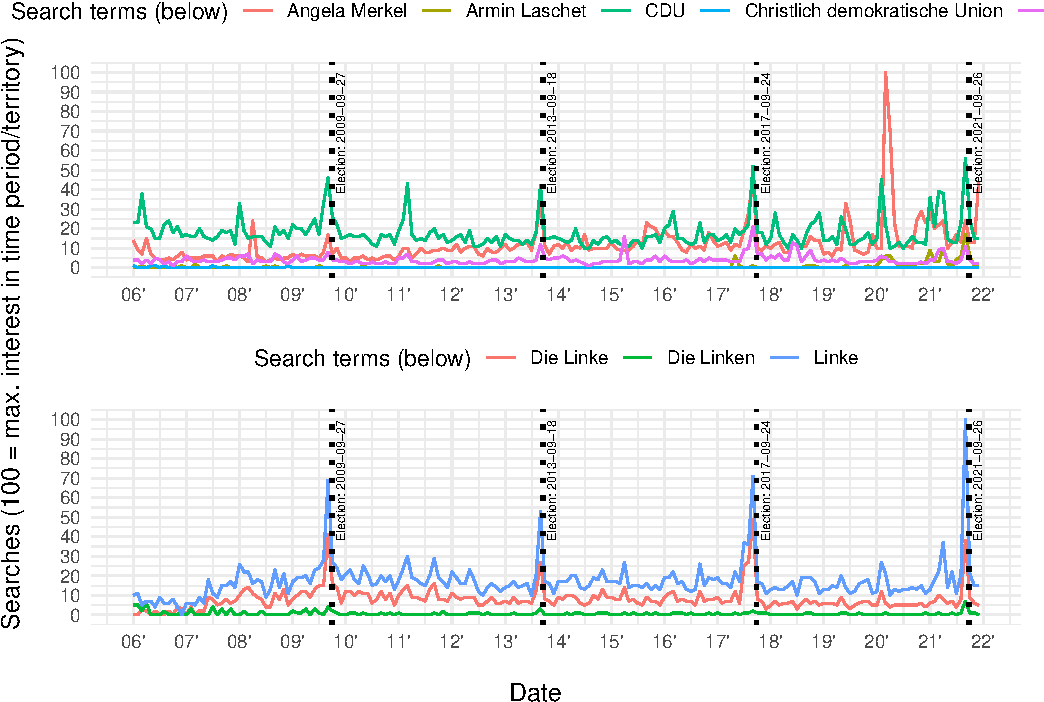
\includegraphics{figures/fig-1-1.pdf}

}

\end{figure}

In Step 2, we compared all search terms for a party identified in Step 1
to explore how relevant the single search terms were in relation to the
other search terms. The comparison showed that the party abbreviation,
e.g., SPD, is extremely well suited whereas the full party name is not.
Special cases were the parties ``Die Grünen'' and ``Die Linken''. In the
case of the party ``Die Grünen'', the search query ``Grüne'' delivered
the best results, since the use of a category assures that only search
terms in the political context are used and the term already includes
longer and other spellings such as ``Die Grünen'' or ``Bündnis 90 die
Grünen''. As depicted in Figure~\ref{fig-1}, the same can be observed
for the party ``Die Linke'', for which the search query ``Linke'' is
best suited. In addition, using the same strategy as above we found that
the names of the respective leading party candidates yielded even better
predictions for all parties. In the case of dual leadership, both
candidates were added.\footnote{A special case was the party ``Die
  Linke,'' which nominated eight top candidates in 2013. By comparing
  the search queries of the individual top candidates separately, we
  filtered out the only two top candidates that seemed relevant for the
  prediction, who were ``Gregor Gysi'' and ``Sarah Wagenknecht.''} The
final search queries of a party are made up of the party abbreviation and
the top candidate(s), which are linked with the ``+'' operator. This
functions according to the scheme of an OR operation, i.e., it sums up
the search interest for each individual term. In step 3, we compared the
predictive power of a set of search terms containing both the party
abbreviation and the top candidate with another set containing only the
party abbreviations. We found that the additional consideration of the
top candidates provided significantly better results.\footnote{Regarding
  the number of terms within a search query for a party, one could argue
  that the result of a search query should be divided by the number of
  search terms, because the search queries of some parties contain more
  individual terms and could thus be overrepresented (e.g.~if a party
  has a dual leadership). In our opinion, this argumentation is not
  plausible, because the search terms for one party never provide an
  equal share of the search interest. The share of the term for the
  party abbreviation is much higher than that for the party candidates,
  so it is illogical to treat them equally. We checked this scenario by
  searching only for the more popular candidate when there is a dual
  leadership, which results in the same amount of search terms for each
  party. This, however, leads to much worse predictions than our main
  analysis. Thus, we assume that the parties are not overrepresented by
  their multiple top candidates.} Table~\ref{tbl-2} displays the final
search queries.

\hypertarget{tbl-2}{}
\begin{table}
\caption{\label{tbl-2}Final search queries }\tabularnewline

\centering\begingroup\fontsize{10}{12}\selectfont

\begin{tabular}{l>{\raggedright\arraybackslash}p{5in}}
\toprule
Election date & Search queries\\
\midrule
2009-09-27 & CDU + CSU + Angela Merkel; SPD + Frank Walter Steinmeier; Grüne + Jürgen Trittin + Renate Künast; Linke + Gregor Gysi; FDP + Guido Westerwelle\\
2013-09-22 & c("CDU + CSU + Angela Merkel", "SPD + Peer Steinbrück", "Jürgen Trittin + Katrin Göring Eckardt + Grüne + ", "Linke + Sarah Wagenknecht + Gregor Gysi", "FDP + Philipp Rösler"); c("Bernd Lucke + Afd", "CDU + CSU + Angela Merkel", "SPD + Peer Steinbrück", "Jürgen Trittin + Katrin Göring Eckardt + Grüne", "FDP + Philipp Rösler")\\
2017-09-24 & c("CDU + CSU + Angela Merkel", "SPD + Martin Schulz", "Cem Özdemir + Katrin Göring Eckardt + Grüne", "Linke + Sarah Wagenknecht + Dietmar Bartsch", "FDP + Christian Lindner"); c("Alice Weidel + Alexander Gauland + Afd", "CDU + CSU + Angela Merkel", "SPD + Martin Schulz", "Cem Özdemir + Katrin Göring Eckardt + Grüne", "FDP + Christian Lindner")\\
2021-09-26 & c("CDU + CSU + Armin Laschet", "SPD + Olaf Scholz", "Annalena Baerbock + Grüne", "Linke + Janine Wissler + Dietmar Bartsch", "FDP + Christian Lindner"); c("Alice Weidel + Tino Chrupalla + Afd", "CDU + CSU + Armin Laschet", "SPD + Olaf Scholz", "Annalena Baerbock + Grüne", "FDP + Christian Lindner")\\
\bottomrule
\end{tabular}
\endgroup{}
\end{table}

\hypertarget{sec-gtdatacollection}{%
\subsection{Collecting GT data}\label{sec-gtdatacollection}}

To collect data on GT, we use the R package ``gtrendsR'' (Massicotte \&
Eddelbuettel, 2023). For the purpose of our analysis we rely on the
comparison function of GT. In the following, the term ``request(s)''
implies that we collect data from GT using this function. Unfortunately,
Google Trends only allows us to compare up to five groups of terms at a
time. In Germany, however, the total number of major political parties
in Germany amounts to six since the appearance of the party AfD in 2013.
For the respective elections (2013-2021) we conducted two requests: The
first request included our search queries for the major political parties
CDU, SPD, FDP, ``Die Grünen'' and ``Die Linke.'' The second request is
similar to the first one, with the difference that we exchanged ``Die
Linke'' with AfD, in order to get data for the AfD. Since, the relative
scale for the comparative GT data is always anchored (setting the
maximum) using the most popular search term, we can leave out or
exchange search terms as it does not change their popularity relative to
the maximum. As a result we get estimates of search interest for all six
parties. Table~\ref{tbl-2} displays the final search queries. We
collected Google Trends data, having set the geo-location to Germany,
for our search queries from the first day of an election year until the
26th September for 2009, 2013, 2017 and 2021. Additionally we collected
data from the election year 2005, which we later used to construct a
weighting factor.\footnote{Choosing a period longer than 270 days for
  the election our years, results in getting weekly data instead of
  daily data. One might also ask if it would make a difference to pull
  one dataset that covers all interval and distance combinations, as in
  our case, or to pull single datasets for each interval and distance
  combination. We checked this and it made no difference since we only
  use the comparison function of Google Trends. Accordingly, the ratio
  of the parties to each other remains the same (30).}

\hypertarget{google-trends-samples}{%
\subsubsection{Google Trends samples}\label{google-trends-samples}}

Importantly, Google Trends draws new samples of all searches on the
platform several times a week (27). As a result, the data varies
slightly from sample to sample. Google states that the samples taken are
representative of all Google search queries. However, Google does not
provide any information on how this representativeness is achieved (28).
Since Google does not specify at what intervals new samples are taken,
we collected new data sets every hour for several weeks and compared
them. It turned out that new samples were taken at least once a day,
sometimes more often. To account for the variation one may find across
samples, we collect GT data at 10 different time points between 01/12/22
and 10/12/22 (see Table~\ref{tbl-A1} in Section~\ref{sec-gtsampling}).
We compare datasets across time points to assure that we base our
estimates on non-identical datasets as to account for sampling error. In
our data analysis, we then use the average values across those datasets
as well as the associated confidence intervals. Surprisingly, we are the
first study within the election prediction literature to acknowledge
this problem, although it is an obvious source of error (30).
Figure~\ref{fig-A2} in Section~\ref{sec-gtsampling} visualizes the
variation of the 10 GT datasets. Moreover, in contrast to statements in
the literature referring to data from the Google Trends website (32) and
the GTEfH API (33), we find that sometimes more than one different
sample can be obtained on the same day (see Table~\ref{tbl-A1} in
Section~\ref{sec-gtsampling}) and that drawing samples from different
PCs in different networks at the same time yields the same sample when
using gtrendsR.

\hypertarget{google-trends-data-windows}{%
\subsubsection{Google trends data
windows}\label{google-trends-data-windows}}

After having collected data from 1 January to 27 September of each
election year, the question arises which data windows within these data
are best suited for election prediction. As depicted in
Figure~\ref{fig-2}, data windows are defined by their width (length of
time period) and distance to the election. In previous research authors
rarely provided a justification for the corresponding choices.

\begin{figure}[h]

\caption{\label{fig-2}Logic of Google Trends data windows}

{\centering 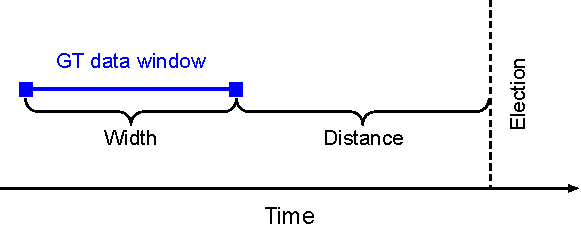
\includegraphics{Figure_2_data_window_logic.pdf}

}

\end{figure}

In what concerns width, the majority of studies used time window(s) with
a width of 1/2 weeks or 1/3 months. In contrast, our aim is to
systematically examine as many data windows as possible in order to find
the best possible prediction windows and to provide guidance for future
research. In doing so we compare small with large data windows. Small
data windows better reflect the searches occurring in short time spans
and the current mood in those time periods. Wider data windows reflect
average interest across a longer time period and average out
non-meaningful spikes (e.g., TV appearances). We compare data windows of
eight widths namely 7, 14, 21, 28, 42, 56, 70 and 91 days.\\
In what concerns distance, previous studies have barely examined this
aspect and have mostly chosen a distance of one day to the election.
However, election campaign leaders and demoscopists will be more
interested in how parties are predicted to perform at an earlier
timepoint, e.g., two weeks or three months before the election. We
compare the predictive power of GT data windows of distance one to 150
days before election day. For instance, a distance of, e.g., 30 days
means that the GT data window ends 30 days before the election. In
total, we compare 8 (number of widths) * 150 (number of distances) =
1200 different GT data windows per election.

\hypertarget{sec-polldatacollection}{%
\subsection{Collecting polling and election
data}\label{sec-polldatacollection}}

In addition to Google Trends data we also collected polling data both as
a comparison for our Google Trend predictions but also to weight our
Google Trends predictions. The polling data comes from one of the most
reputable German polling institutes, Infratest dimap. Finally, the
outcome we want to predict are actual election results. We collected the
corresponding data from the official source of the federal government
(Bundeswahlleiter 2023).

\hypertarget{sec-models}{%
\subsection{Prediction models and benchmark}\label{sec-models}}

In our analysis, we predict party shares in four federal elections in
Germany: 2009, 2013, 2017 and 2021. We build three broad classes of
predictive models:\\
Our first class of models, MC1, consists of the raw, unweighted Google
Trends data; The second class of models, MC2, uses a weighting factor
based on the results of the preceding election; Our last class of
models, MC3, weights the GT predictions using polling results of
Infratest dimap, which will be explained in more detail below. In total
we estimate 4 (elections) * 3 (model classes) * 1200 (data windows) =
14400 models. We compare predictions of models based on GT data to
predictions based on models drawing on polls for the time windows to
benchmark their performance.\footnote{The term model does not
  necessarily refer to a sophisticated statistical model here. For
  instance, the models based on polls are simply the party shares as
  measured in the polls.} For each election, we compare our predictions
for the single parties with the actual election results. Below we
visualize and evaluate both errors across our models for single parties
\(y_{p}-\hat{y}_{p}\) as well as averaged across parties using the
\(MAE = \frac{\sum_{i=1}^{n}|y_{p}-\hat{y}_{p}|}{n}\) where \(p\)
corresponds to a party and \(y_{p}\) and \(\hat{y}_{p}\) to the true and
predicted party share respectively.\\
MC1 models predict party shares solely with Google Trends data. To
obtain these we proceeded as follows: We started by calculating the
Google proportion for each party \(p\) for a data window \(i\). As shown
in Eq. 1, in the first step, we use the average Google search interest of
each party \(p\) for the examined data window \(i\), for example, the
average search interest for the search query of the CDU for the data
window with width 7 days and distance 7 days. Then we divide it by the
sum \(N\) of all parties average search interest for that data window.
The Google proportion thus serves as a prediction in percent for the
respective party.

\[\text{Google Proportion}_{p,i}=\frac{\text{Avg. Google search interest}_{p,i}}{\sum_{p=1}^{N} \text{Avg. Google search interest}_{p,i}}\text{ (Eq. 1)}\]

If we add up the Google proportions of all the parties examined, we
arrive at 100\%. This Google proportion serves as the sole basis for
models of class MC1. Highlighting our strategy reveals a slight
disadvantage of our analysis data compared to the election polls. While
the election polls also include the category ``Other,'' which in extreme
cases can go up to 8.7\% of the votes, we lack this category on GT. This
means that in the polls the main parties can sometimes only get 91.3\%,
whereas in our analysis they get 100\%. As a result, we assume that
party shares are slightly overestimated in the GT data. We provide
additonal analyses constructing an ``other'' category from google search
data in Section~\ref{sec-other-parties} finding that the results do not
change much. In our conclusion we discuss possible ways of how the
``other'' category could be accounted for when collecting GT data.\\
For models of class MC2 and MC3 we use weighting factors in conjunction
with the party shares predicted by GT proportions. Models of class MC2
are based on the approach of Polykalas et al. (22), who used the results
of the previous federal election to calculate a weighting factor. As
shown in \(Eq. 2\), to calculate the weighting factor \(WMC2\) for a
party \(p\), for the data window \(i\) and the election year \(T\), we
divide the previous election results of that party \(p\) of the previous
election year \(T-4\) by the respective Google proportion. For example,
to predict the SPD's share in 2017 we must first calculate the weighting
factor \(WMC2\). For that, we take the SPD's election result in 2013 and
divide it by the GT proportion of the SPD for the election of 2013 using
the same distance d and width w for the respective data window i.
Subsequently, the GT prediction of the SPD's 2017 share, is multiplied
by the weighting factor \(WMC2\) of the SPD. The result is the
prediction provided by M2 for the SPD's share in 2017.

\[\text{Weight}_{MC2(p,i,T)}=\frac{\text{Previous election results}_{p,T-4}}{\text{Google proportionp}_{i,T-4}}\text{ (Eq. 2)}\]

\(\text{Weight}_{MC2(p,i,T)}\) partly may account for the possible
selection that characterizes individuals that end up in the GT data by
including information on shares in the previous election (4 years
earlier) in Germany. For instance, non-Internet users are probably
underrepresented and younger voters over-represented among GT users.
Because the electorate changes for each election, we cannot assume that
this weighting method controls/offsets the complete sample bias for the
election year we want to predict. But it should provide better
predictions than models of class MC1 that are solely based on GT
data.\footnote{A special case is MC2 for the 2013 election, for which
  the 2009 election is used to calculate the weighting factor. The party
  AfD was founded in 2013, as a consequence, we do not have data from
  2009. We circumvented this problem by not weighting the AfD's Google
  proportion in 2013, which should be taken into account when looking at
  the results.} In our opinion, this class of models is justified
insofar it uses GT and previous election data for the prediction and no
other external data.

\begin{figure}[h]

\caption{\label{fig-3}Weighting logic underlying models of class MC3}

{\centering 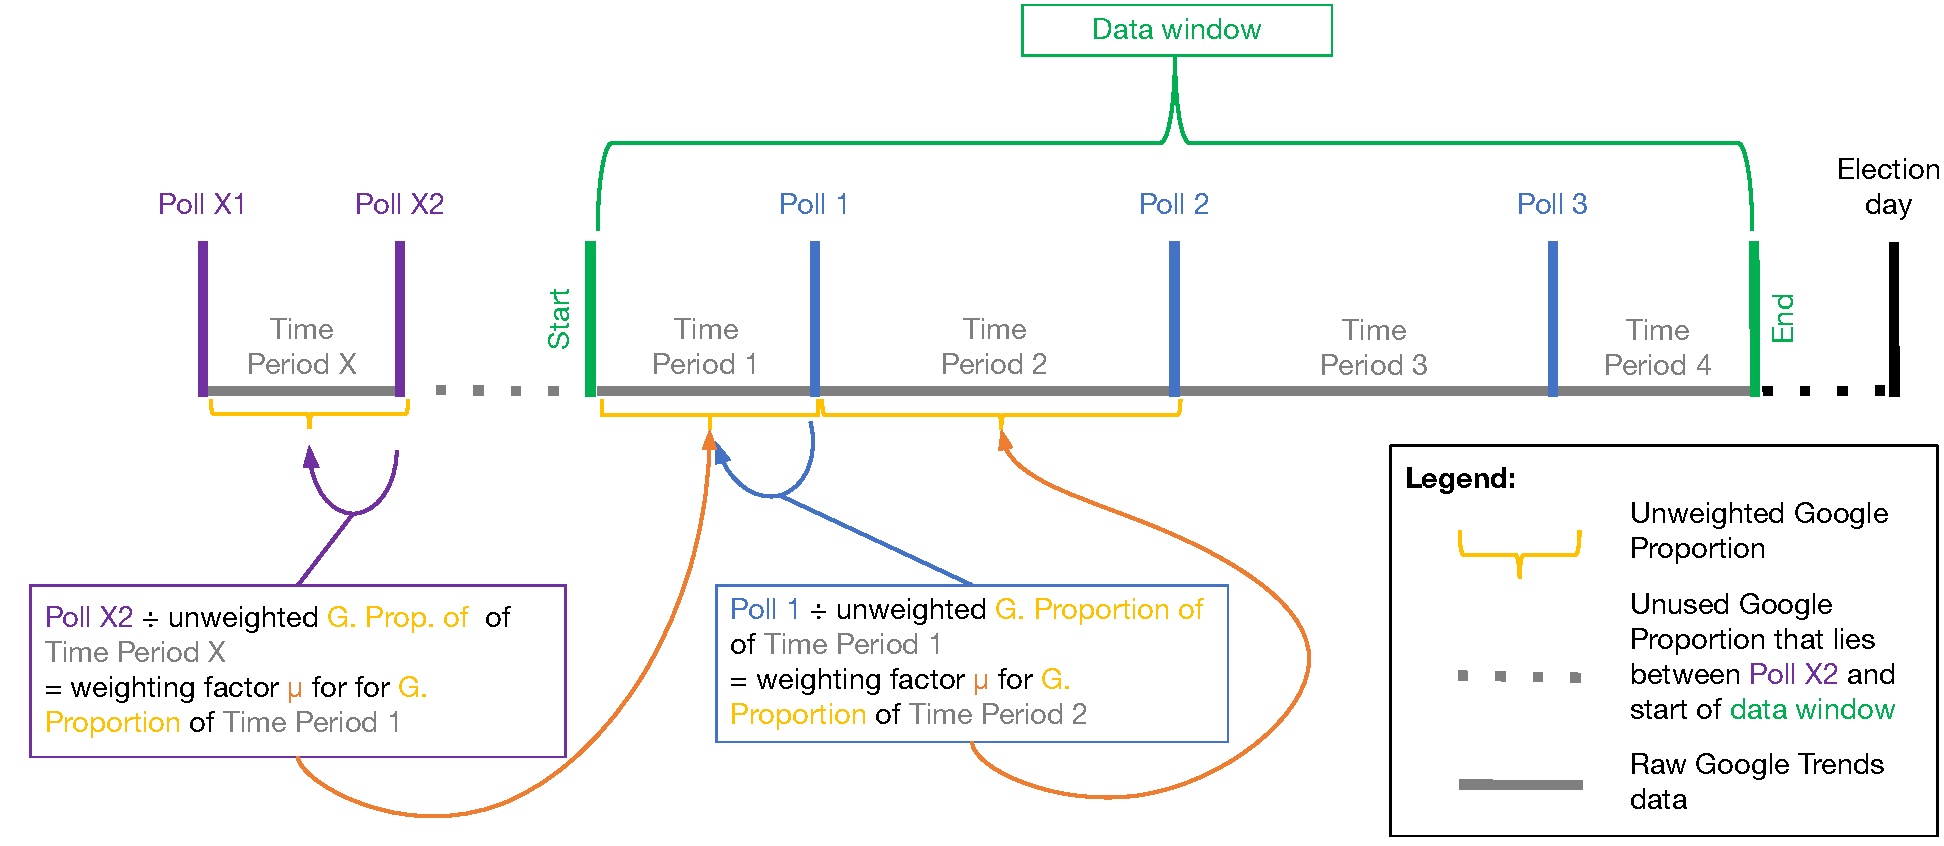
\includegraphics{Figure_3_weighting_logic.pdf}

}

\end{figure}

For models of class MC3, we use polling data from the Infratest Dimap
institute for weighting, which is normally published every two
weeks.\footnote{Occasionally in 1 or 3 week intervals.} This enables us
to calculate a new weighting factor every two weeks, which corrects for
possible over- or underestimates in the GT data. This is especially true
for short-term trends due to specific events (e.g.~television
appearances) that lead to an increase in search queries. The weighting
factor is calculated similarly to the previous weighting factor, except
that in this case we are looking at slices of two weeks of data (the
period from one survey to the next).\footnote{In the actual data the
  polls do not appear exactly every two weeks.} The weighting scheme
underlying MC3 models is illustrated in Figure~\ref{fig-3}.
Figure~\ref{fig-3} depicts a data window that contains three election
polls, Poll 1-3. Poll 1-3 slice the data window into Time periods 1-4.
Moreover, there is polls before the data window namely Poll X1 and X2.
We always weight the GT data (proportions) of a time period, e.g., Time
Period 2 with a weighting factor. As shown in Eq. 3, the weighting
factor consists of the poll at the start of this time period (here Poll
1) divided by the GT data (proportions) of the previous time period
(here Time Period 1). We do the same for the other time periods within
the data window, i.e., Time Periods 2 and 3.

\[\text{Weight}_{MC3(t ‐ t+1)}=\frac{\text{Poll}_{\text{Time Period x}}}{\text{Google proportion}_{\text{Time Period x - 1}}}\text{ (Eq. 2)}\]

Time Period 1 is special insofar that in most cases the start date of
the time window and a poll do not lie on the same date. Therefore the
Google proportion between the start of the interval and the 1st poll
(here Poll 1) in the time window cannot be weighted. Therefore, we
utilize the last poll before the time window (here Poll X2) to calculate
the weighting factor. The Google Proportion needed for the weighting
factor is thereby limited by the two last polls before the time window
(here Poll X1 and X2, resulting in Time Period X).\footnote{If there is
  no poll in our data window, we use the first poll before the data
  window. In the case where the start time of the data window and a poll
  fall on the same day, the Google proportion up to the 1st poll before
  the data window is used and divided by the poll falling on the same
  day as the start time to calculate the weighting factor. Subsequently,
  the Google proportion starting one day after the start date and poll
  up to the first poll in the interval is weighted. Polls that fall on
  the same day as the end day of an interval are ignored because it
  wouldn't make sense to calculate a weighting factor using only one day
  of Google data and applying it on the same day.}

\hypertarget{sec-results}{%
\section{Results}\label{sec-results}}

\hypertarget{comparing-predictions-across-gt-data-windows-across-parties}{%
\subsection{Comparing predictions across GT data windows, across
parties}\label{comparing-predictions-across-gt-data-windows-across-parties}}

We start by comparing MC1 models that solely based on GT data, varying
the GT data windows both in terms of width, i.e., the number of days
covered by the respective GT dataset, and distance, i.e., the number of
days the window is away from the election.

\begin{figure}[H]

\caption{\label{fig-4}Accuracy of GT predictions for different parties
and party shares across data windows}

{\centering 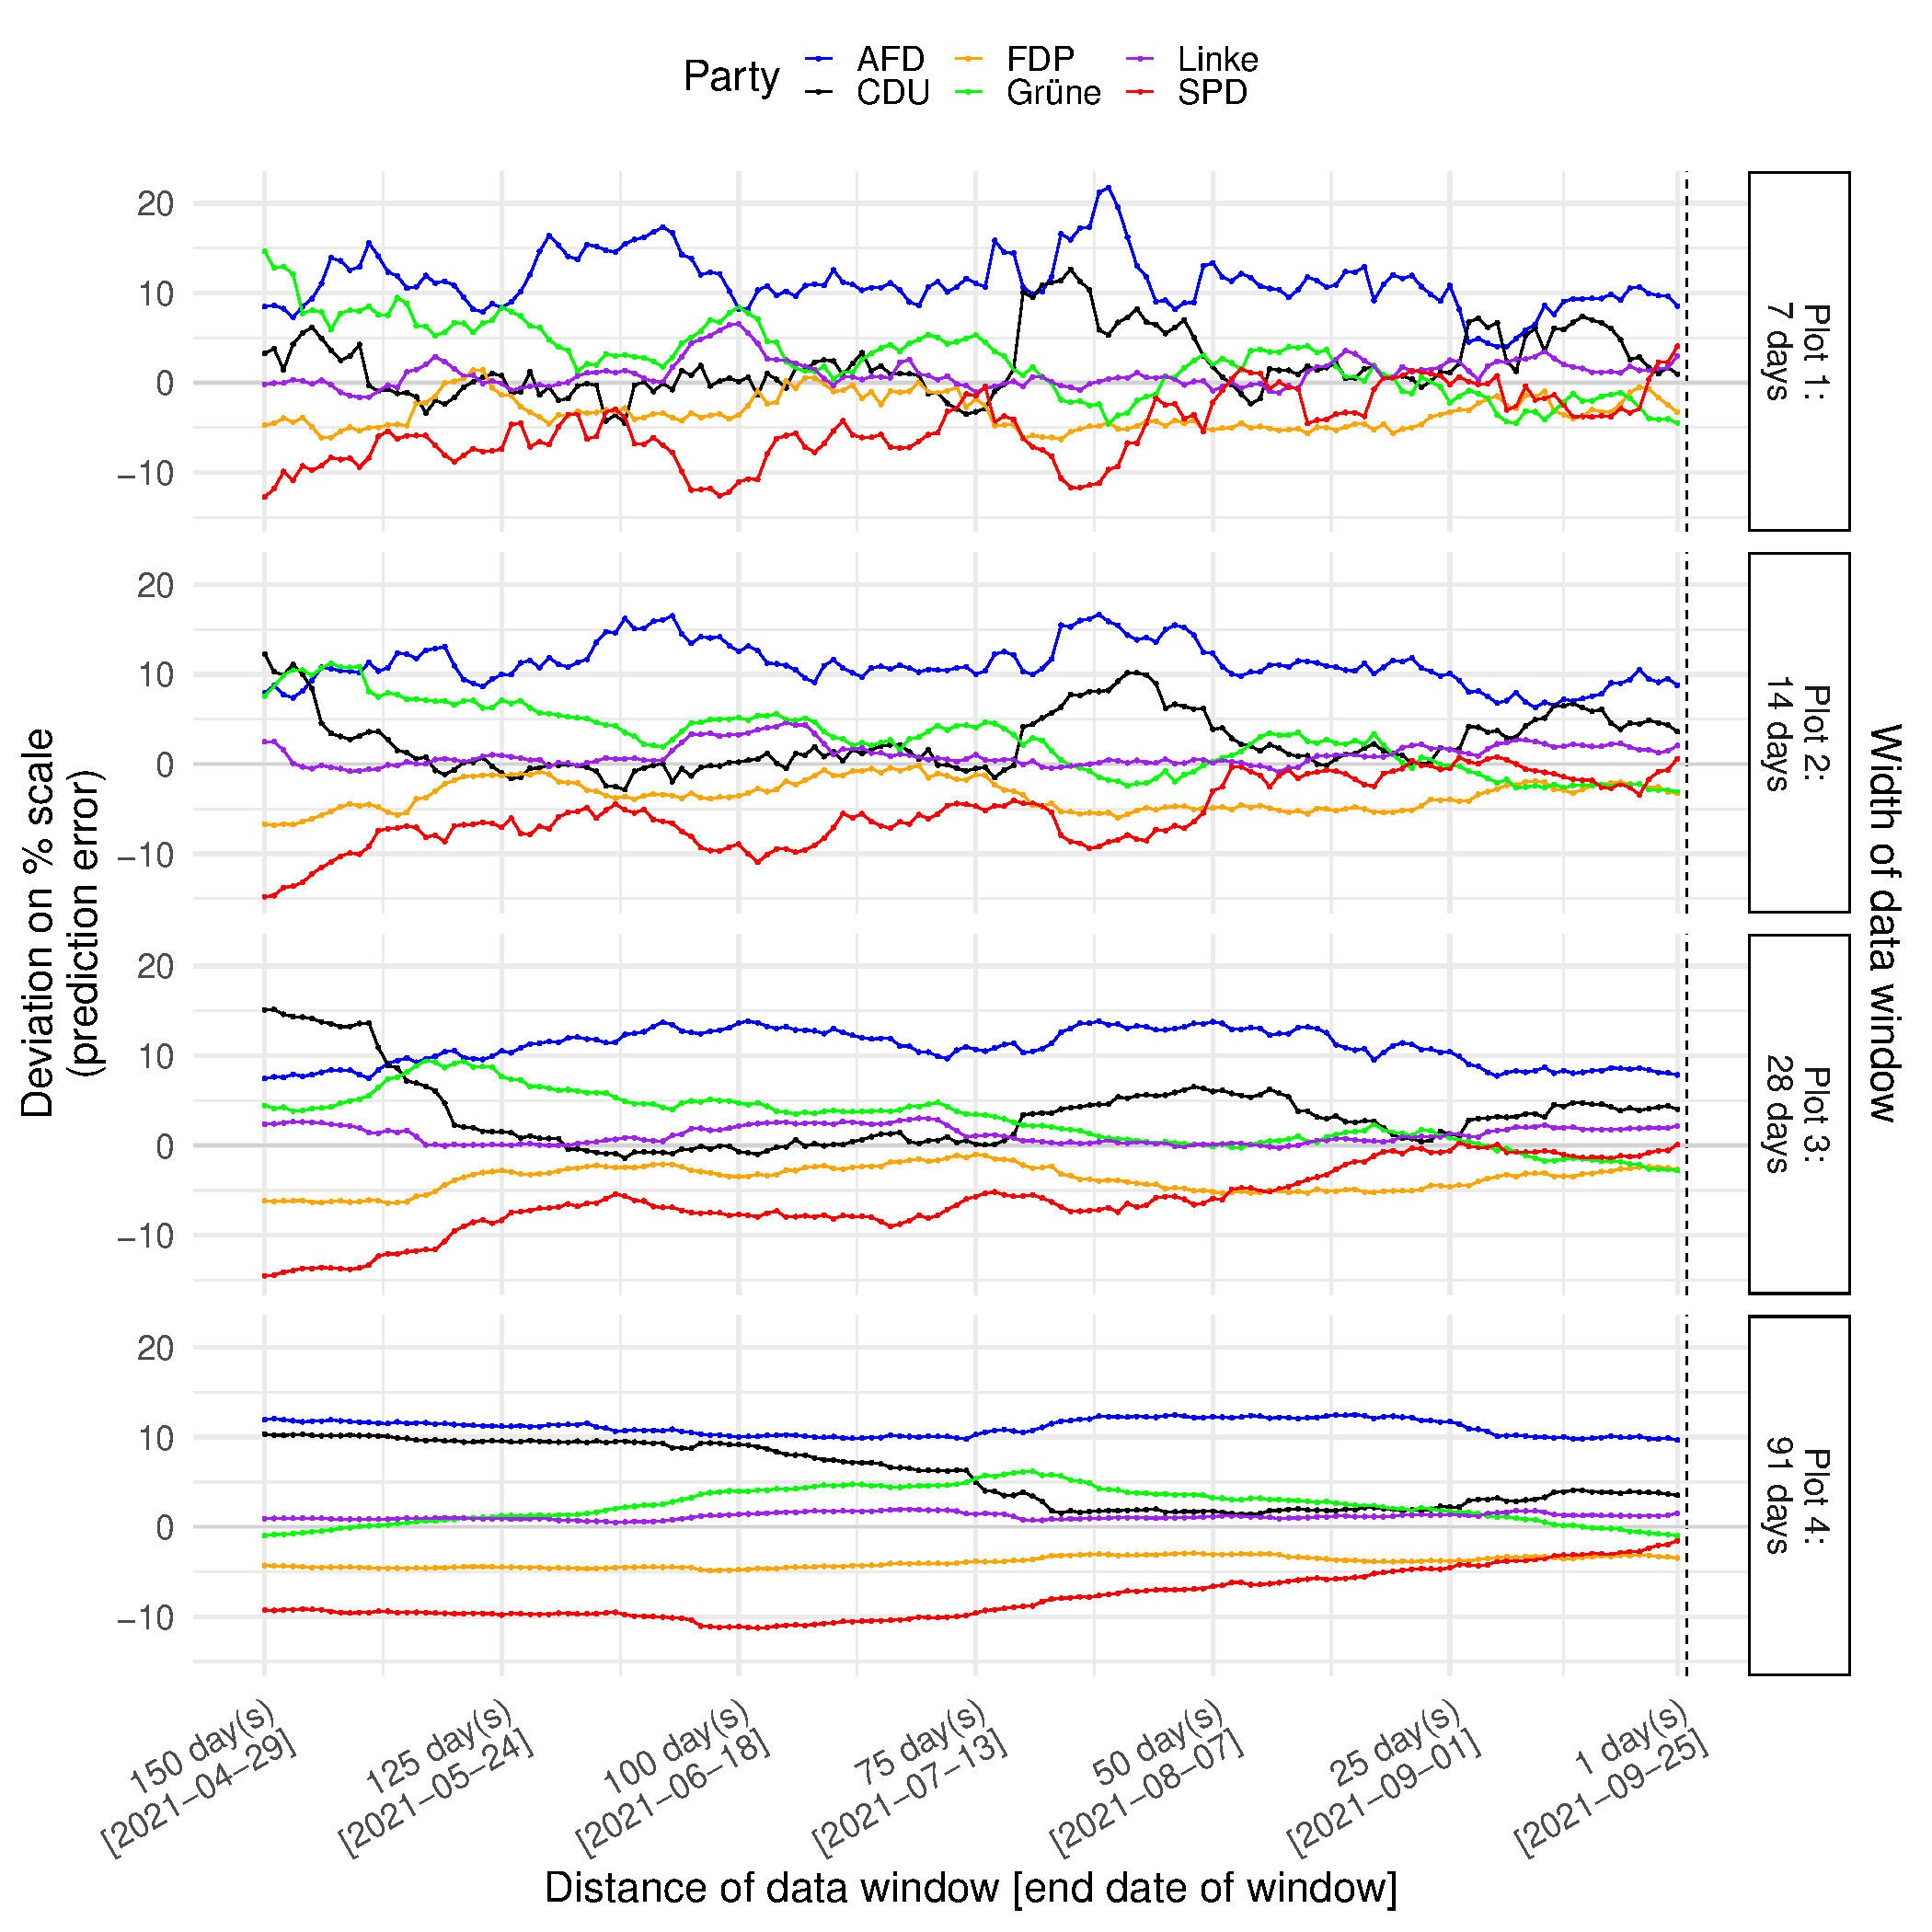
\includegraphics{figures/fig-4-1.pdf}

}

\end{figure}

In Figure~\ref{fig-4} we visualize a subset of the predictions provided
by MC1-GT models for the most recent general election in Germany (26th
of September 2021). The most recent election is ideal for benchmarking
GT predictions, because usage of the platform has changed over time.
Figure~\ref{fig-4} plots the prediction errors \((y_{p}-\hat{y}_{p})\)
as points connected by lines for 3600 predictions = 6 parties * 600
models (defined by 4 widths and 150 distances).\footnote{Obtained by
  averaging predictions over 10 GT data samples.}\footnote{The graph is
  only showing a subset of our predictions restricted to one election
  and four data window widths. Overall, from our models that are solely
  based on GT data we yielded 27600 predictions, namely predictions for
  6 parties of based on 4800 models defined by 8 widths, 150 distances
  and 4. For the 2009 election, we have 21600 solely GT data based
  predictions. For the 2013, 2017, 2021 elections we obtained 21600
  predictions.}

The single panels (Plot 1-4) correspond to the four different widths of
the data windows going from 7 days to 91 days (see right-hand y-axis).
The x-axis indicates the distance of the respective window to the
election. First, we find that the width and distance of the data window
to the election matters. We compare models of differing width (from top
to bottom) and distance (from left to right). Data windows of low width,
e.g., the models based on 7 days of GT data in the top plot, vary much
stronger in their predictive accuracy across time. In other words, with
such small time spans it matters which week of GT data we have picked
for our prediction. Naturally, this variation decreases when we extend
the time window on which we base our prediction going from 7 days (Plot
1) to 91 days (Plot 4) at the bottom in Figure~\ref{fig-4}. Second, on
average accuracy seems to improve slightly the smaller the distance
between the GT data window and the election. In Figure~\ref{fig-5} we
plot the prediction error averaged across all parties for MC1-GT models
(red line) contrasting them with other models. Focusing on the red line
this analysis also indicates that the error decreases the closer we are
to the election. However, we can also clearly see that picking a short
data window, e.g., 7 days, results in considerable variation in what
regards accuracy (see Figure~\ref{fig-4}, Plot 1).\\
In addition, we used a linear model to model the trend of accuracy as a
function of distance holding the width constant at 14 days in
Table~\ref{tbl-A2}. For the 2021 election, the average error decreases
by 0.02\% per day distance. In other words, if move the data window 100
days closer to the election, the mean absolute error decreases by 2\%.
This, however, is not true for the other elections (cf.
Table~\ref{tbl-A2}). Third, Figure~\ref{fig-4} also highlights the
strong variation in accuracy between parties. For instance, GT
predictions of the vote share of the Linke are more accurate than, e.g.,
for the AFD, with the error being closer to 0 across models. For the
2021 election the error generally seems highest for the AfD. Moreover,
shares of certain parties are usually underestimated (e.g., SPD), while
others are overestimated (e.g., AfD). It seems that the quality of
Google searches as a signal of vote choice differs across parties.
Importantly, Figure~\ref{fig-A4} provides further visualizations for
more intervals for the 2021 election, Figure~\ref{fig-A5} provide
visualizations for the other elections and Table~\ref{tbl-A2} also
provides models for the other elections. The insights described above
are largely confirmed when using data for other elections.

\hypertarget{comparing-predictions-across-model-classes}{%
\subsection{Comparing predictions across model
classes}\label{comparing-predictions-across-model-classes}}

Above, we compared different models within class MC1-GT focusing on the
width and distance of data windows. Previous studies have often combined
GT data with election or polling data. As described in
Section~\ref{sec-models} we compare predictions across three broad
classes of models. Figure~\ref{fig-5} again focuses on the 21' election.

\begin{figure}[H]

\caption{\label{fig-5}Comparing the accuracy of different modelling
approaches}

{\centering 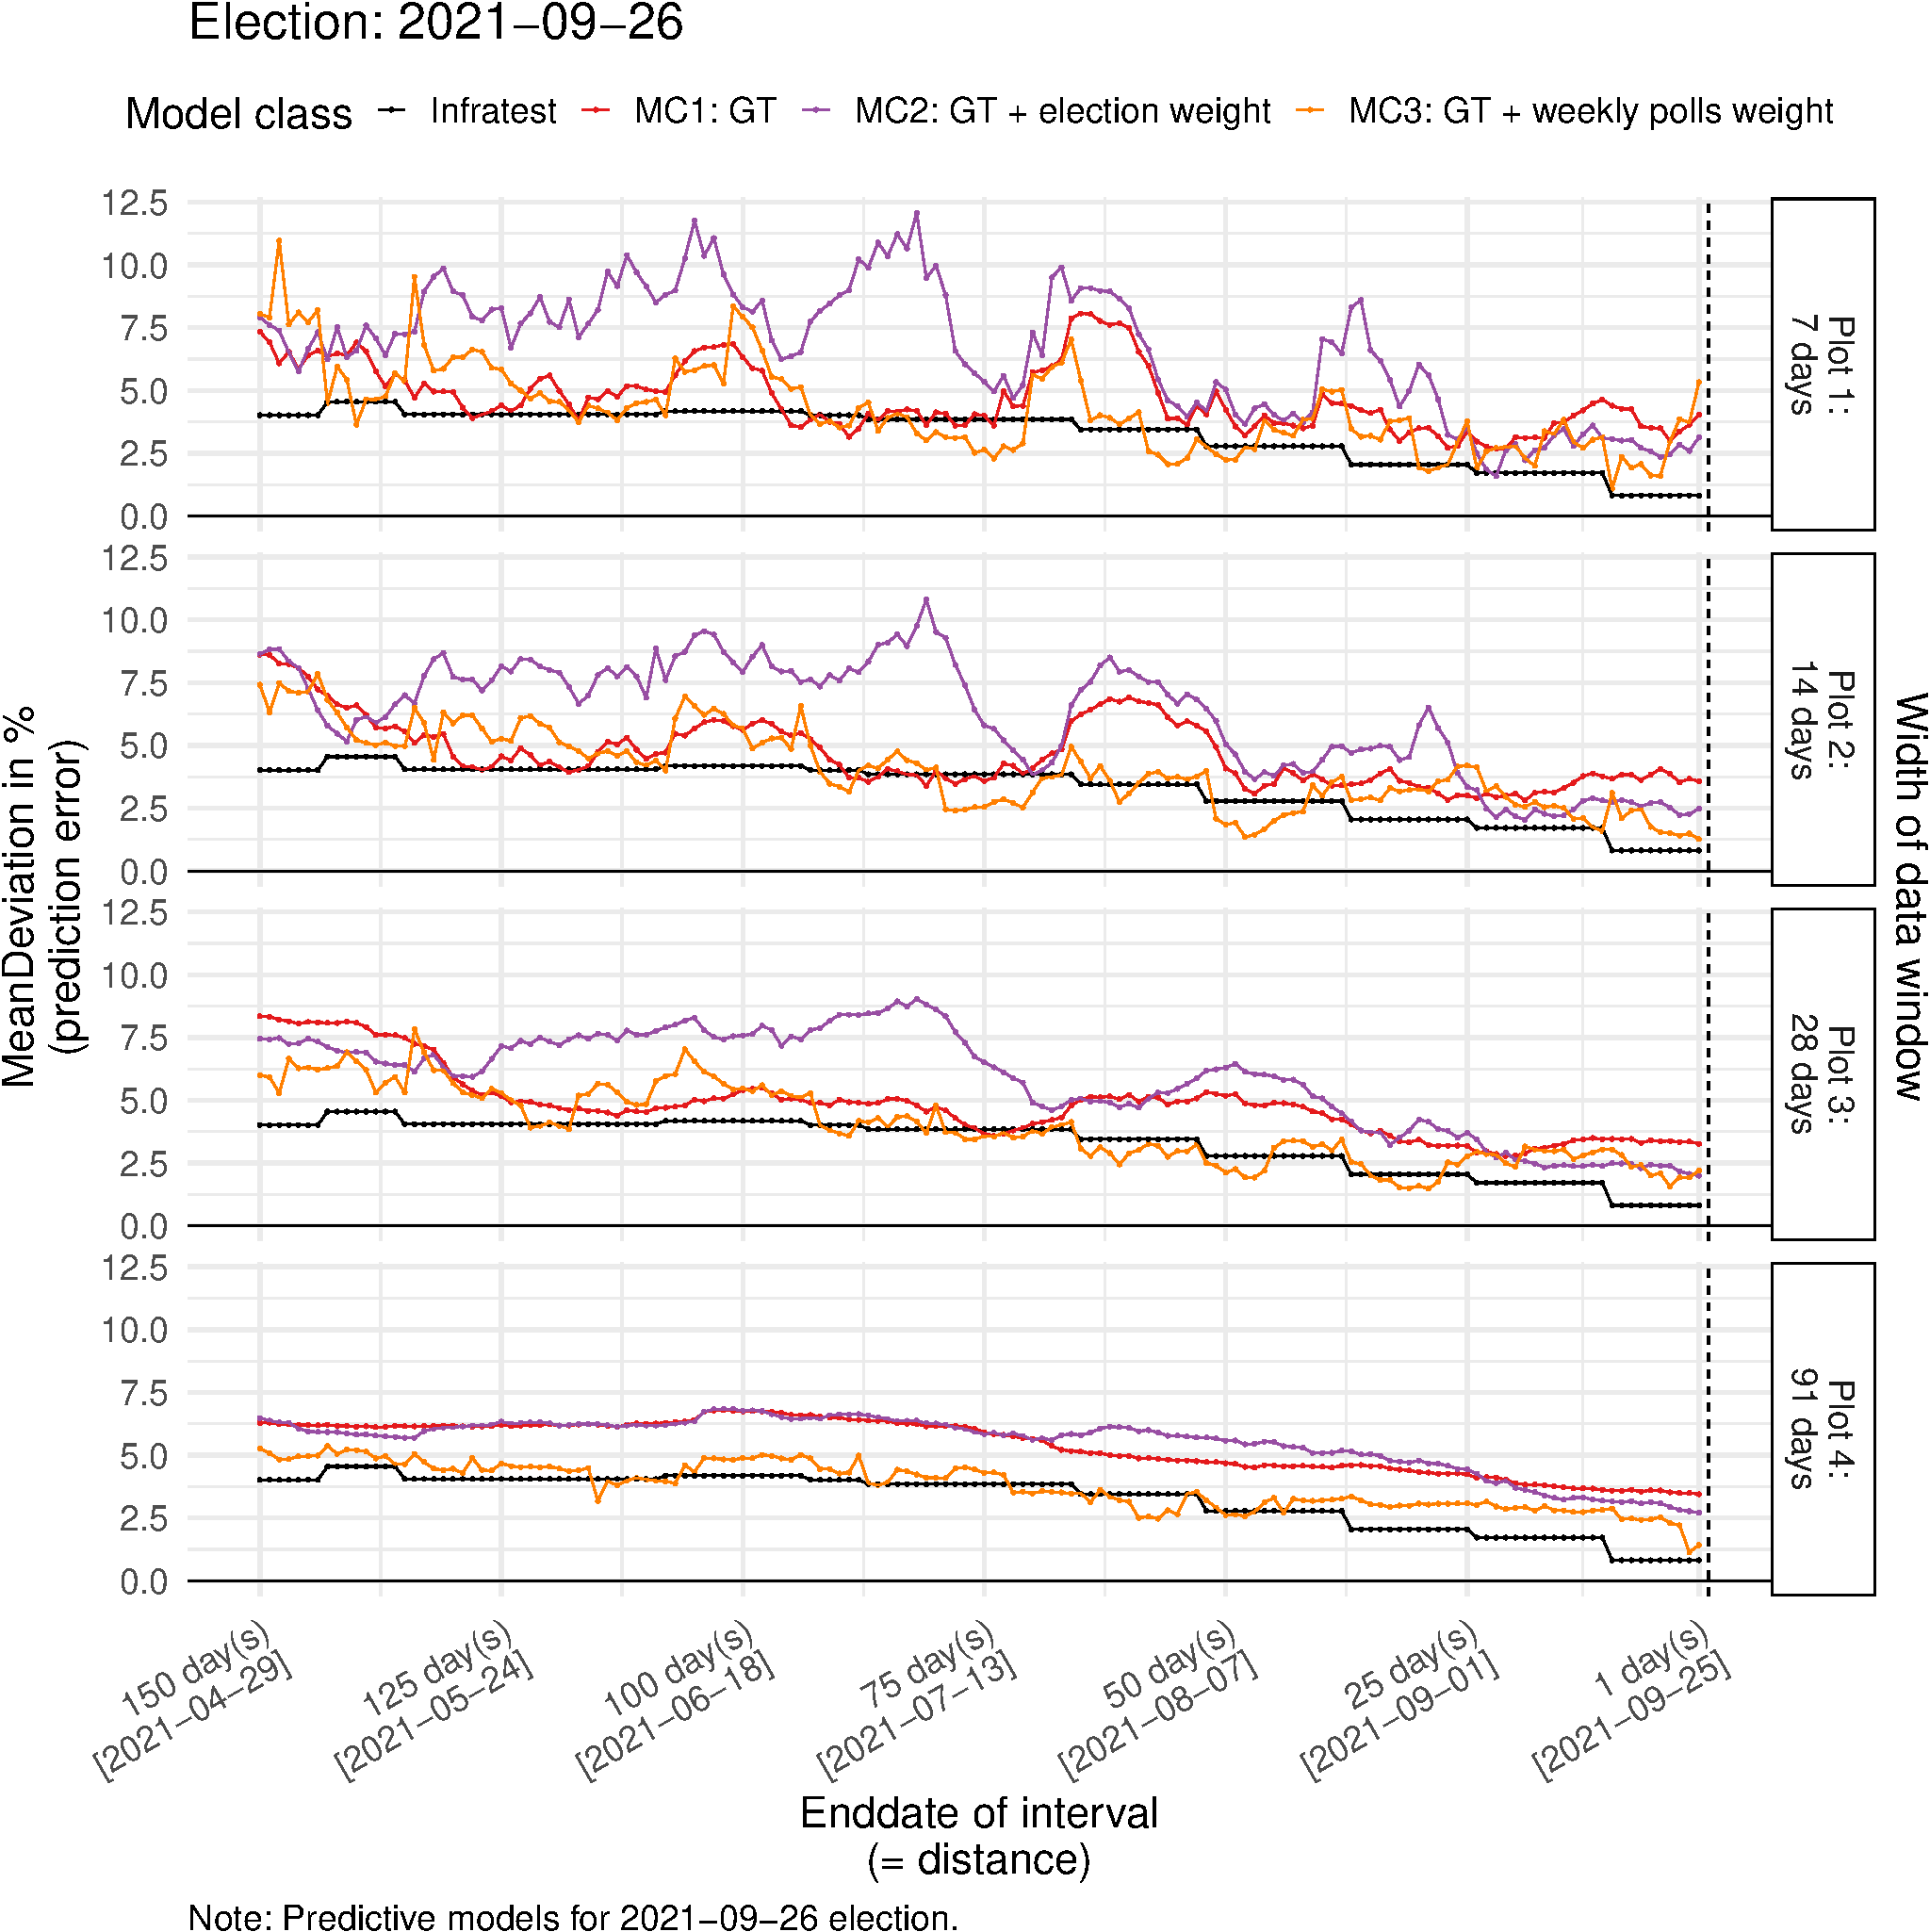
\includegraphics{figures/fig-5-1.pdf}

}

\end{figure}

Now, each point represents the mean absolute error, i.e., the prediction
error averaged across parties. Figure~\ref{fig-5} visualizes 2400
predictions (150 distances * 4 intervals * 4 models including
Infratest). The models are colored: MC1 models based on GT data in red,
MC2 models based on GT data weighted with previous election results in
purple, MC3 models based on GT data weighted with polling data in
orange. Finally, we have the predictions based on Infratest Dimap polls
(colored in black), whereby we simply use the last Dimap poll in the
respective time windows.\\
As in Figure~\ref{fig-4}, the four plots in Figure~\ref{fig-5} (Plot
1-4) correspond to different widths of the data window. No surprisingly,
we find that polls (black line) unarguably perform the best for the 2021
election reflected in the fact that prediction error mostly scores below
our GT data based models of Class MC1-3. In Figure~\ref{fig-3} this
becomes visible as the black line is almost always closer to 0 then the
other ones.\\
We also compared how often our other models actually provide better
predictions. GT data based MC1 models provide better prediction in 6\%
(35 out of 600) of the cases. MC2 models that weight GT data with
previous election perform the worst with 0\% (2 out of 600) better
predictions as compared to polls by Infratest Dimap. Finally, MC3 models
that combine GT data with polls perform the best with 24\% (147 out of
600) of predictions being better. The picture hardly changes when we
restrict our models to those based on a width of 91 days.\\
Naturally, we could discuss whether the accuracy of our GT based models
(MC1) is really so much worse than polling data given the latter's
costs. We can collect GT data for free, errors of the size found here
may be acceptable for certain applications where we only need rough
predictions. Besides, if we want to decrease the dependency of GT-based
predictions on short-term trends we should probably base our predictions
on a larger time span as shown in Plot in Figure~\ref{fig-3}. We provide
findings for other elections in
Section~\ref{sec-comparison-models-elections} and in
Section~\ref{sec-comparing-model-classes-other}.

\hypertarget{sec-comparison-models-elections}{%
\subsection{Comparing predictions across model classes and
elections}\label{sec-comparison-models-elections}}

Above we focused on the most recent election in Germany (9th of
September 2021). This focus is justified: Given the changing user
population, the most recent election is the most appropriate to assess
the predictive power of GT search data. Nonetheless, a comparison with
earlier elections can provide us with some insights as to what
variations we can expect for coming elections. Figure~\ref{fig-6} is
similar to Figure~\ref{fig-5} only that the width of the data window is
held constant at 91 days which corresponds to Plot 4 in
Figure~\ref{fig-5}, and predictions for different elections are shown on
top of each other (Plot 1-4). Again, each point represents the mean
absolute error, i.e., the prediction error averaged across parties
whereby predictions by different model classes are colored.

\begin{figure}[H]

\caption{\label{fig-6}Accuracy of predictions across model classes and
election}

{\centering 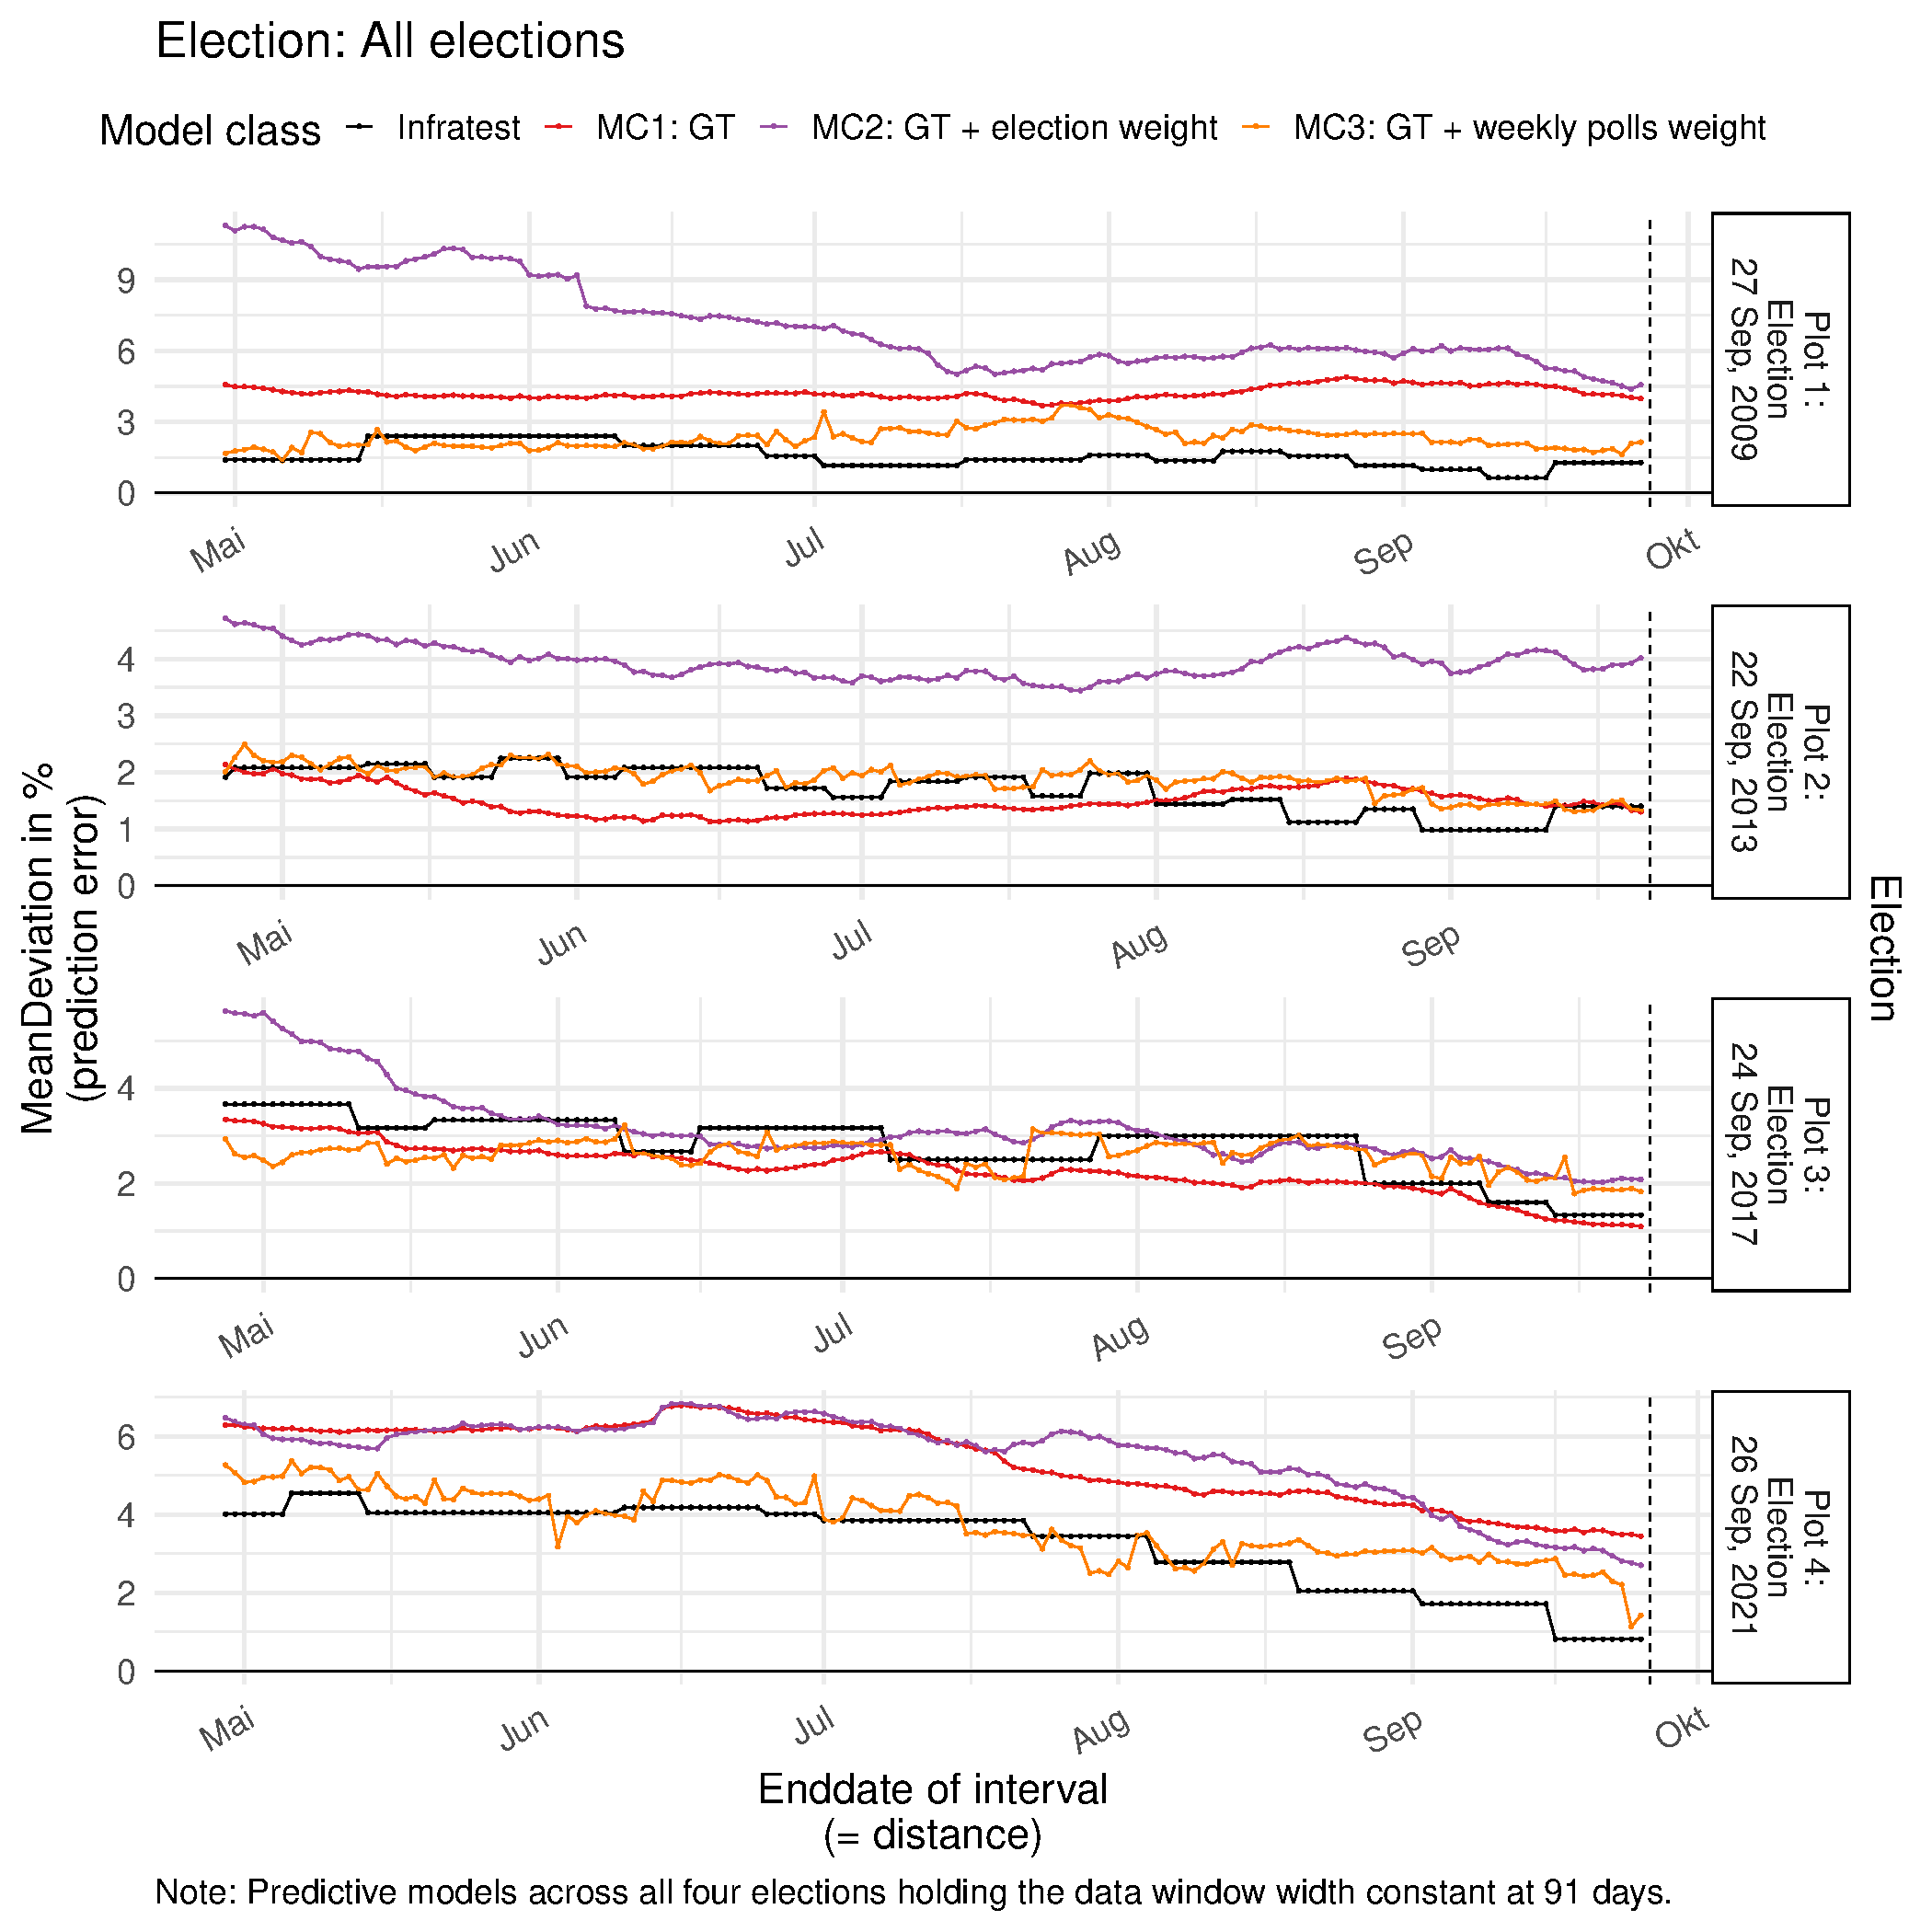
\includegraphics{figures/fig-6-1.pdf}

}

\end{figure}

\hypertarget{tbl-3}{}
\begin{table}
\caption{\label{tbl-3}Comparing model predictions to polls }\tabularnewline

\centering\begingroup\fontsize{9}{11}\selectfont

\begin{tabular}{ll>{\raggedright\arraybackslash}p{1in}>{\raggedright\arraybackslash}p{1in}}
\toprule
Model class & Election & Better predictions: \% & Better predictions: n out of total\\
\midrule
MC1: GT & 2009 & 0\% & 0 out of 150\\
 & 2013 & 66\% & 99 out of 150\\
 & 2017 & 97\% & 145 out of 150\\
 & 2021 & 0\% & 0 out of \vphantom{1} 150\\
MC2: GT + election weight & 2009 & 0\% & 0 out of 150\\
\addlinespace
 & 2013 & 0\% & 0 out of 150\\
 & 2017 & 32\% & 48 out of 150\\
 & 2021 & 0\% & 0 out of 150\\
MC3: GT + weekly polls weight & 2009 & 20\% & 30 out of 150\\
 & 2013 & 29\% & 43 out of 150\\
\addlinespace
 & 2017 & 73\% & 109 out of 150\\
 & 2021 & 20\% & 30 out of 150\\
\bottomrule
\end{tabular}
\endgroup{}
\end{table}

We find that indeed the accuracy of predictions varies across elections.
Table~\ref{tbl-3} provides an overview regarding how often the different
models where better than purely poll based predictions across elections
(poll based predictions always concern the last poll). We can see that
2021 and 2009 were particular bad years for models of class MC1 and MC2
with zero better predictions than polls. In contrast, models of class
MC3 provided better predictions for 20\% of the estimated models both in
2009 and 2021. For the 2013 election, the purely GT data based models
beat the polls in 66\% of the estimated models and provide better
predictions than the other model classes most of the time. For the 2017
election, the purely GT data based models fare even better, beating the
polls in 97\% of the models (defined by width and distance), with the
other two model classes faring somewhat worse. Hence, in general, 2017
was a particularly bad year for the polls in our data.\\
We can only speculate why there is such strong variation across
elections. First, as mentioned, we have to assume that the
representativity of Google search users varies across time. In
principle, it is possible that the population of Google search users was
more representative of German voters in the 2013, 2017 elections than in
2009 or 2021. Second, it could be related to the elections themselves.
Potentially, the extend to which the action ``search for'' is related to
``vote for'' depends on the election with more ``charged'' elections
like the 2021 election decreasing this correlation (34). Third, it is
possible that the accuracy of the polling data which we use as a
benchmark varies over time.

\hypertarget{sec-conclusion}{%
\section{Conclusion}\label{sec-conclusion}}

Google trends data has become a popular data source for prediction in
different domains such as elections. While most previous research
focuses on binary electoral outcomes such as referendum results or
presidential elections, we evaluate GT predictions in a multi-party
setting. We developed a framework that allows us to compare predictions
across 1200 fine-grained GT data windows that vary both in terms of
width (7 to 91 days) and distance to the election (1 to 150 days). And,
we compare predictions across several elections (four general elections
in Germany). Besides, we provide a more systematic assessment hitherto
neglected choices such as the selection of search terms, GT data samples
and search refinement categories. Tackling these different dimensions
allows us to provide some unique insights. First, we find that
predictive accuracy varies significantly as a function of the width and
distance of GT data windows. To some extent disagreement on the
predictive accuracy of GT data in previous research may be linked to the
varying choices researchers made here (cf. Table~\ref{tbl-2}). In what
concerns width(s), accuracy varies significantly across time for shorter
data windows (here 7-28 days). We would generally recommend choosing
larger data windows for predictive purposes to average out variation
that is due to singular events. And, akin to classic polling data we
find that predictive accuracy increases the closer our data window to
the election. Second, in terms of predictive models we compared models
based on GT data, on GT + previous electoral outcomes data and GT +
opinion poll data. Generally, high quality opinion polls, in our case by
the renowned company Infratest Dimap, still represents the benchmark in
terms of accuracy, especially in the case of the latest election in
2021. We found that models that combine polling data with GT data (MC3)
data fare better than purely GT-data-based models (MC1). Furthermore, we
find that weighting GT data with previous electoral outcomes (22) does
not help predictive accuracy, at least not for the German case (cf.
Figure~\ref{fig-3}). Third, while we argued that recent elections are
the appropriate benchmarks for GT data predictions, comparisons to past
elections may still be revealing. Especially, insofar our findings for
the 2021 election are somewhat discouraging, which goes against earlier
studies that emphasize the predictive accuracy of GT data. Hence, we
need to test whether our findings for 2021 also hold for other
elections. And, especially for the 2013 and 2017 election GT data models
where much more accurate, at times beating or at least aligning with
predictions based on opinion polls (cf. Figure~\ref{fig-6}). Above we
speculated that the nature of the election may affect the predictive
power of GT data (cf. 34). More generally, this highlights that
conclusions regarding predictive accuracy from one election may not
generalize to other elections. Finally, we conclude that GT prediction
research should ideally become more. From our review we learned that
identifying the various characteristics in Table~\ref{tbl-2}, i.e., all
representing important choices when using GT data, was a challenge.
Future research would benefit if authors would report more details,
e.g., the exact time of GT data collection, the number of GT samples,
the nature of search term selection. For instance, we found that it
matters which category search filter is selected (see
Section~\ref{sec-categoryfilterselection}).\\
Our study has several limitations that provide venues for future
research. First, we pursued a systematic approach to search term
selection, testing different search terms against each other (see
Section~\ref{sec-searchterms}). Future research might benefit from
choosing an even wider net of search terms, trying out different ones.
Second, while we predicted elections shares we did not forecast them in
that the elections happened already. Since, we didn't built any
sophisticated models we somewhat circumvented the danger of adapting our
models to already seen data. Nonetheless, as is now more common in the
literature on election forecasting (8), studies that rely on GT data for
prediction could also be pre-registered. Third, from the general
perspective of election forecasting, GT data could be seen as just
another dynamic signal that can be integrated into more sophisticated
modelling strategies (e.g., 10) that go beyond the simple weighting
approach used in the present paper. Whether such additional sources of
data can improve predictions remains to be tested. Fourth, the changing
predictive power of GT across elections maybe related to (1) how
representative the GT data is of searches on the platform and (2) how
representative users of the GT platform are of voting the population.
Pertaining to (1), both aspects of representiveness should be studied
further. Finding variation across GT data samples Raubenheimer et al.
(27) suggested that there might be a publication bias, i.e., successful
predictions are based on suitable samples. For this reason we averaged
across GT data samples (cf. Section~\ref{sec-gtdatacollection} and
Section~\ref{sec-gtsampling}). However, more rearch into the variability
of such samples for particular predictions is warranted. However, user
representativity (2) is relevant as well. Platforms are generally quite
secretive about their userbase. Collecting more evidence on how
representative Goodle users are of the general (voting) population would
help to explain the accuracy of corresponding predictions and help to
develop more sophisticated weighting schemes.

\newpage

\hypertarget{references}{%
\section{References}\label{references}}

\hypertarget{refs}{}
\begin{CSLReferences}{0}{0}
\leavevmode\vadjust pre{\hypertarget{ref-choi_predicting_2012}{}}%
\CSLLeftMargin{1. }%
\CSLRightInline{Choi H, Varian H. Predicting the present with {Google}
{Trends}. Economic record. 2012;88:2--9. }

\leavevmode\vadjust pre{\hypertarget{ref-ginsberg_detecting_2009}{}}%
\CSLLeftMargin{2. }%
\CSLRightInline{Ginsberg J, Mohebbi MH, Patel RS, Brammer L, Smolinski
MS, Brilliant L. Detecting influenza epidemics using search engine query
data. Nature {[}Internet{]}. 2009 Feb {[}cited 2023 Jan
30{]};457(7232):1012--4. Available from:
\url{http://www.nature.com/articles/nature07634}}

\leavevmode\vadjust pre{\hypertarget{ref-askitas_calling_2015}{}}%
\CSLLeftMargin{3. }%
\CSLRightInline{Askitas N. Calling the {Greek} {Referendum} on the
{Nose} with {Google} {Trends}. SSRN Electronic Journal {[}Internet{]}.
2015; Available from: \url{https://doi.org/10.2139\%2Fssrn.2708382}}

\leavevmode\vadjust pre{\hypertarget{ref-askitas_predicting_2015}{}}%
\CSLLeftMargin{4. }%
\CSLRightInline{Askitas N. Predicting the {Irish}'{Gay}
{Marriage}'{Referendum}. Available at SSRN 2674243. 2015; }

\leavevmode\vadjust pre{\hypertarget{ref-mavragani_yes_2016}{}}%
\CSLLeftMargin{5. }%
\CSLRightInline{Mavragani A, Tsagarakis KP. {YES} or {NO}: {Predicting}
the 2015 {GReferendum} results using {Google} {Trends}. Technological
Forecasting and Social Change {[}Internet{]}. 2016;109:1--5. Available
from:
\url{https://www.sciencedirect.com/science/article/pii/S0040162516300580}}

\leavevmode\vadjust pre{\hypertarget{ref-mavragani_predicting_2019}{}}%
\CSLLeftMargin{6. }%
\CSLRightInline{Mavragani A, Tsagarakis KP. Predicting referendum
results in the {Big} {Data} {Era}. Journal of Big data. 2019;6(1):1--20.
}

\leavevmode\vadjust pre{\hypertarget{ref-prado-roman_google_2021}{}}%
\CSLLeftMargin{7. }%
\CSLRightInline{Prado-Román C, Gómez-Martínez R, Orden-Cruz C. Google
trends as a predictor of presidential elections: The {United} {States}
versus {Canada}. American Behavioral Scientist. 2021;65(4):666--80. }

\leavevmode\vadjust pre{\hypertarget{ref-gschwend_zweitstimme_2022}{}}%
\CSLLeftMargin{8. }%
\CSLRightInline{Gschwend T, Müller K, Munzert S, Neunhoeffer M, Stoetzer
LF. The {Zweitstimme} model: {A} dynamic forecast of the 2021 {German}
federal election. PS: Political Science \& Politics. 2022;55(1):85--90.
}

\leavevmode\vadjust pre{\hypertarget{ref-munzert_zweitstimme_2017}{}}%
\CSLLeftMargin{9. }%
\CSLRightInline{Munzert S, Stötzer L, Gschwend T, Neunhoeffer M,
Sternberg S. Zweitstimme. Org. {Ein} strukturell-dynamisches
{Vorhersagemodell} für {Bundestagswahlen}. Politische
Vierteljahresschrift. 2017;418--41. }

\leavevmode\vadjust pre{\hypertarget{ref-stoetzer_forecasting_2019}{}}%
\CSLLeftMargin{10. }%
\CSLRightInline{Stoetzer LF, Neunhoeffer M, Gschwend T, Munzert S,
Sternberg S. Forecasting elections in multiparty systems: A {Bayesian}
approach combining polls and fundamentals. Political Analysis.
2019;27(2):255--62. }

\leavevmode\vadjust pre{\hypertarget{ref-jennings_election_2018}{}}%
\CSLLeftMargin{11. }%
\CSLRightInline{Jennings W, Wlezien C. Election polling errors across
time and space. Nature Human Behaviour {[}Internet{]}. 2018
Apr;2(4):276--83. Available from:
\url{https://doi.org/10.1038/s41562-018-0315-6}}

\leavevmode\vadjust pre{\hypertarget{ref-schnell_accuracy_2014}{}}%
\CSLLeftMargin{12. }%
\CSLRightInline{Schnell R, Noack M.
\href{https://doi.org/10.12758/mda.2014.001}{The accuracy of
pre-election polling of {German} general elections}. Methods, data,
analyses : a journal for quantitative methods and survey methodology
(mda). 2014;8(1):5--24. }

\leavevmode\vadjust pre{\hypertarget{ref-wang_forecasting_2015}{}}%
\CSLLeftMargin{13. }%
\CSLRightInline{Wang W, Rothschild D, Goel S, Gelman A. Forecasting
elections with non-representative polls. International Journal of
Forecasting {[}Internet{]}. 2015;31(3):980--91. Available from:
\url{https://www.sciencedirect.com/science/article/pii/S0169207014000879}}

\leavevmode\vadjust pre{\hypertarget{ref-Granka2013-mu}{}}%
\CSLLeftMargin{14. }%
\CSLRightInline{Granka L. Using online search traffic to predict {US}
presidential elections. PS Polit Sci Polit. 2013 Apr;46(2):271--9. }

\leavevmode\vadjust pre{\hypertarget{ref-initiative_d21_share_2022}{}}%
\CSLLeftMargin{15. }%
\CSLRightInline{D21 I. Share of internet users in {Germany} from 2001 to
2021 {[}{Graph}{]}. Statista {[}Internet{]}. 2022 {[}cited 2023 Feb
17{]}; Available from:
\url{https://www.statista.com/statistics/380514/internet-usage-rate-germany/}}

\leavevmode\vadjust pre{\hypertarget{ref-statcounter_desktop_2023}{}}%
\CSLLeftMargin{16. }%
\CSLRightInline{StatCounter. Desktop and mobile search market share of
search engines in {Germany} in {December} 2023 {[}{Graph}{]}. Statista
{[}Internet{]}. 2023 {[}cited 2023 Feb 17{]}; Available from:
\url{https://www.statista.com/statistics/445974/search-engines-market-share-of-desktop-and-mobile-search-germany/}}

\leavevmode\vadjust pre{\hypertarget{ref-jun_ten_2018}{}}%
\CSLLeftMargin{17. }%
\CSLRightInline{Jun SP, Yoo HS, Choi S. Ten years of research change
using {Google} {Trends}: {From} the perspective of big data utilizations
and applications. Technological Forecasting and Social Change
{[}Internet{]}. 2018;130:69--87. Available from:
\url{https://www.sciencedirect.com/science/article/pii/S0040162517315536}}

\leavevmode\vadjust pre{\hypertarget{ref-kandula_reappraising_2019}{}}%
\CSLLeftMargin{18. }%
\CSLRightInline{Kandula S, Shaman J.
\href{https://doi.org/10.1371/journal.pcbi.1007258}{Reappraising the
utility of {Google} {Flu} {Trends}.} PLoS computational biology. 2019
Aug;15(8):e1007258. }

\leavevmode\vadjust pre{\hypertarget{ref-lazer_parable_2014}{}}%
\CSLLeftMargin{19. }%
\CSLRightInline{Lazer D, Kennedy R, King G, Vespignani A.
\href{https://doi.org/10.1126/science.1248506}{The {Parable} of {Google}
{Flu}: {Traps} in {Big} {Data} {Analysis}}. Science (New York, NY). 2014
Mar;343:1203--5. }

\leavevmode\vadjust pre{\hypertarget{ref-yang_accurate_2015}{}}%
\CSLLeftMargin{20. }%
\CSLRightInline{Yang S, Santillana M, Kou SC. Accurate estimation of
influenza epidemics using {Google} search data via {ARGO}. Proceedings
of the National Academy of Sciences {[}Internet{]}.
2015;112(47):14473--8. Available from:
\url{https://www.pnas.org/doi/abs/10.1073/pnas.1515373112}}

\leavevmode\vadjust pre{\hypertarget{ref-brodeur_covid-19_2021}{}}%
\CSLLeftMargin{21. }%
\CSLRightInline{Brodeur A, Clark AE, Fleche S, Powdthavee N. {COVID}-19,
lockdowns and well-being: {Evidence} from {Google} {Trends}. Journal of
public economics. 2021;193:104346. }

\leavevmode\vadjust pre{\hypertarget{ref-polykalas_general_2013}{}}%
\CSLLeftMargin{22. }%
\CSLRightInline{Polykalas SE, Prezerakos GN, Konidaris A.
\href{https://doi.org/10.1109/WAINA.2013.155}{A {General} {Purpose}
{Model} for {Future} {Prediction} {Based} on {Web} {Search} {Data}:
{Predicting} {Greek} and {Spanish} {Election}}. In: 2013 27th
{International} {Conference} on {Advanced} {Information} {Networking}
and {Applications} {Workshops}. 2013. p. 213--8. }

\leavevmode\vadjust pre{\hypertarget{ref-harkan_predicting_2021}{}}%
\CSLLeftMargin{23. }%
\CSLRightInline{Harkan AA. Predicting the {Results} of the 2019
{Indonesian} {Presidential} {Election} with {Google} {Trends}. In:
Asia-{Pacific} {Research} in {Social} {Sciences} and {Humanities}
{Universitas} {Indonesia} {Conference} ({APRISH} 2019). Atlantis Press;
2021. p. 1--9. }

\leavevmode\vadjust pre{\hypertarget{ref-wolf_trending_2018}{}}%
\CSLLeftMargin{24. }%
\CSLRightInline{Wolf JT. Trending in the {Right} {Direction}: {Using}
{Google} {Trends} {Data} as a {Measure} of {Public} {Opinion} {During} a
{Presidential} {Election} {[}\{PhD\} \{Thesis\}{]}. Virginia Tech; 2018.
}

\leavevmode\vadjust pre{\hypertarget{ref-polykalas_algorithm_2013}{}}%
\CSLLeftMargin{25. }%
\CSLRightInline{Polykalas SE, Prezerakos GN, Konidaris A. An algorithm
based on {Google} {Trends}' data for future prediction. {Case} study:
{German} elections. IEEE International Symposium on Signal Processing
and Information Technology. 2013;000069--73. }

\leavevmode\vadjust pre{\hypertarget{ref-sjovill_using_2020}{}}%
\CSLLeftMargin{26. }%
\CSLRightInline{Sjövill R. Using {Search} {Query} {Data} to {Predict}
the {General} {Election}: {Can} {Google} {Trends} {Help} {Predict} the
{Swedish} {General} {Election}? 2020. }

\leavevmode\vadjust pre{\hypertarget{ref-raubenheimer_hey_2021}{}}%
\CSLLeftMargin{27. }%
\CSLRightInline{Raubenheimer JE, Riordan BC, Merrill JE, Winter T, Ward
RM, Scarf D, et al. Hey {Google}! Will {New} {Zealand} vote to legalise
cannabis? {Using} {Google} {Trends} data to predict the outcome of the
2020 {New} {Zealand} cannabis referendum. International Journal of Drug
Policy {[}Internet{]}. 2021 Apr;90:103083. Available from:
\url{https://doi.org/10.1016\%2Fj.drugpo.2020.103083}}

\leavevmode\vadjust pre{\hypertarget{ref-google_trends_help_faq_2023}{}}%
\CSLLeftMargin{28. }%
\CSLRightInline{Help GT. {FAQ} about {Google} {Trends} data - {Trends}
{Help} {[}Internet{]}. 2023 {[}cited 2023 Jan 27{]}. Available from:
\url{https://support.google.com/trends/answer/4365533?hl=en\&amp\%3Bref_topic=6248052}}

\leavevmode\vadjust pre{\hypertarget{ref-google_trends_help_refine_2023}{}}%
\CSLLeftMargin{29. }%
\CSLRightInline{Help GT. Refine {Trends} results by category - {Trends}
{Help} {[}Internet{]}. 2023 {[}cited 2023 Jan 27{]}. Available from:
\url{https://support.google.com/trends/answer/4359597?hl=en\&amp;ref_topic=4365530}}

\leavevmode\vadjust pre{\hypertarget{ref-eichenauer_obtaining_2022}{}}%
\CSLLeftMargin{30. }%
\CSLRightInline{Eichenauer VZ, Indergand R, Martínez IZ, Sax C.
Obtaining consistent time series from {Google} {Trends}. Economic
Inquiry {[}Internet{]}. 2022;60(2):694--705. Available from:
\url{https://onlinelibrary.wiley.com/doi/abs/10.1111/ecin.13049}}

\leavevmode\vadjust pre{\hypertarget{ref-Behnen2020-tf}{}}%
\CSLLeftMargin{31. }%
\CSLRightInline{Behnen P, Kessler R, Kruse F, Gómez JM, Schoenmakers J,
Zerr S. Experimental evaluation of scale, and patterns of systematic
inconsistencies in google trends data. In: {ECML} {PKDD} 2020 workshops.
Springer International Publishing; 2020. p. 374--84. }

\leavevmode\vadjust pre{\hypertarget{ref-Stephens-Davidowitz2014-qr}{}}%
\CSLLeftMargin{32. }%
\CSLRightInline{Stephens-Davidowitz S, Varian H. A hands-on guide to
google data. further details on the construction can be found on the
Google Trends page. 2014; }

\leavevmode\vadjust pre{\hypertarget{ref-Raubenheimer2022-xe}{}}%
\CSLLeftMargin{33. }%
\CSLRightInline{Raubenheimer JE. A {PRACTICAL} {ALGORITHM} {FOR}
{EXTRACTING} {MULTIPLE} {DATA} {SAMPLES} {FROM} {GOOGLE} {TRENDS}
{EXTENDED} {FOR} {HEALTH}. Am J Epidemiol. 2022 Aug;191(9):1666--9. }

\leavevmode\vadjust pre{\hypertarget{ref-faas_german_2022}{}}%
\CSLLeftMargin{34. }%
\CSLRightInline{Faas T, Klingelhöfer T.
\href{https://doi.org/10.1080/01402382.2022.2045783}{German politics at
the traffic light: New beginnings in the election of 2021}. West
European Politics. 2022;45(7):1506--21. }

\end{CSLReferences}

\newpage

\scalebox{2}{Online appendix}

\beginsupplement

\hypertarget{sec-categoryfilterselection}{%
\section{Category filter selection and search
terms}\label{sec-categoryfilterselection}}

As discussed in Section~\ref{sec-categoryfilter}, Google trends allows
for restricting searches to certain categories. This is helpful insofar
it allows for restricting the data to Google searches that are more
relevant to the phenomenon we want to predict, i.e., elections. To
identify the best category filter, we proceeded as follows: First we
defined a time period and geographical context, namely the time window
of January 1st to September 26th preceding the respective elections.
Second, we defined a set of search terms namely the abbreviations of the
major political parties (e.g., CDU, SPD, etc.). We drew 10 different GT
data samples at different time points to account for any possible
variation across samples. Then for each election year and each sample,
we calculated the Google proportion as explained in
Section~\ref{sec-models} and summed up the corresponding absolute
percentage deviations of each party from the actual election result.
Figure~\ref{fig-A1} visualizes the average absolute percentage deviation
of the Google proportion from the party shares, indicating that
restricting searches to the category ``Law \& Government'' provides the
best predictions. Hence, in our main analysis we further restricted
searches using this category filter.

\begin{figure}[H]

\caption{\label{fig-A1}Category selection among supercategories of
Google Trends}

{\centering 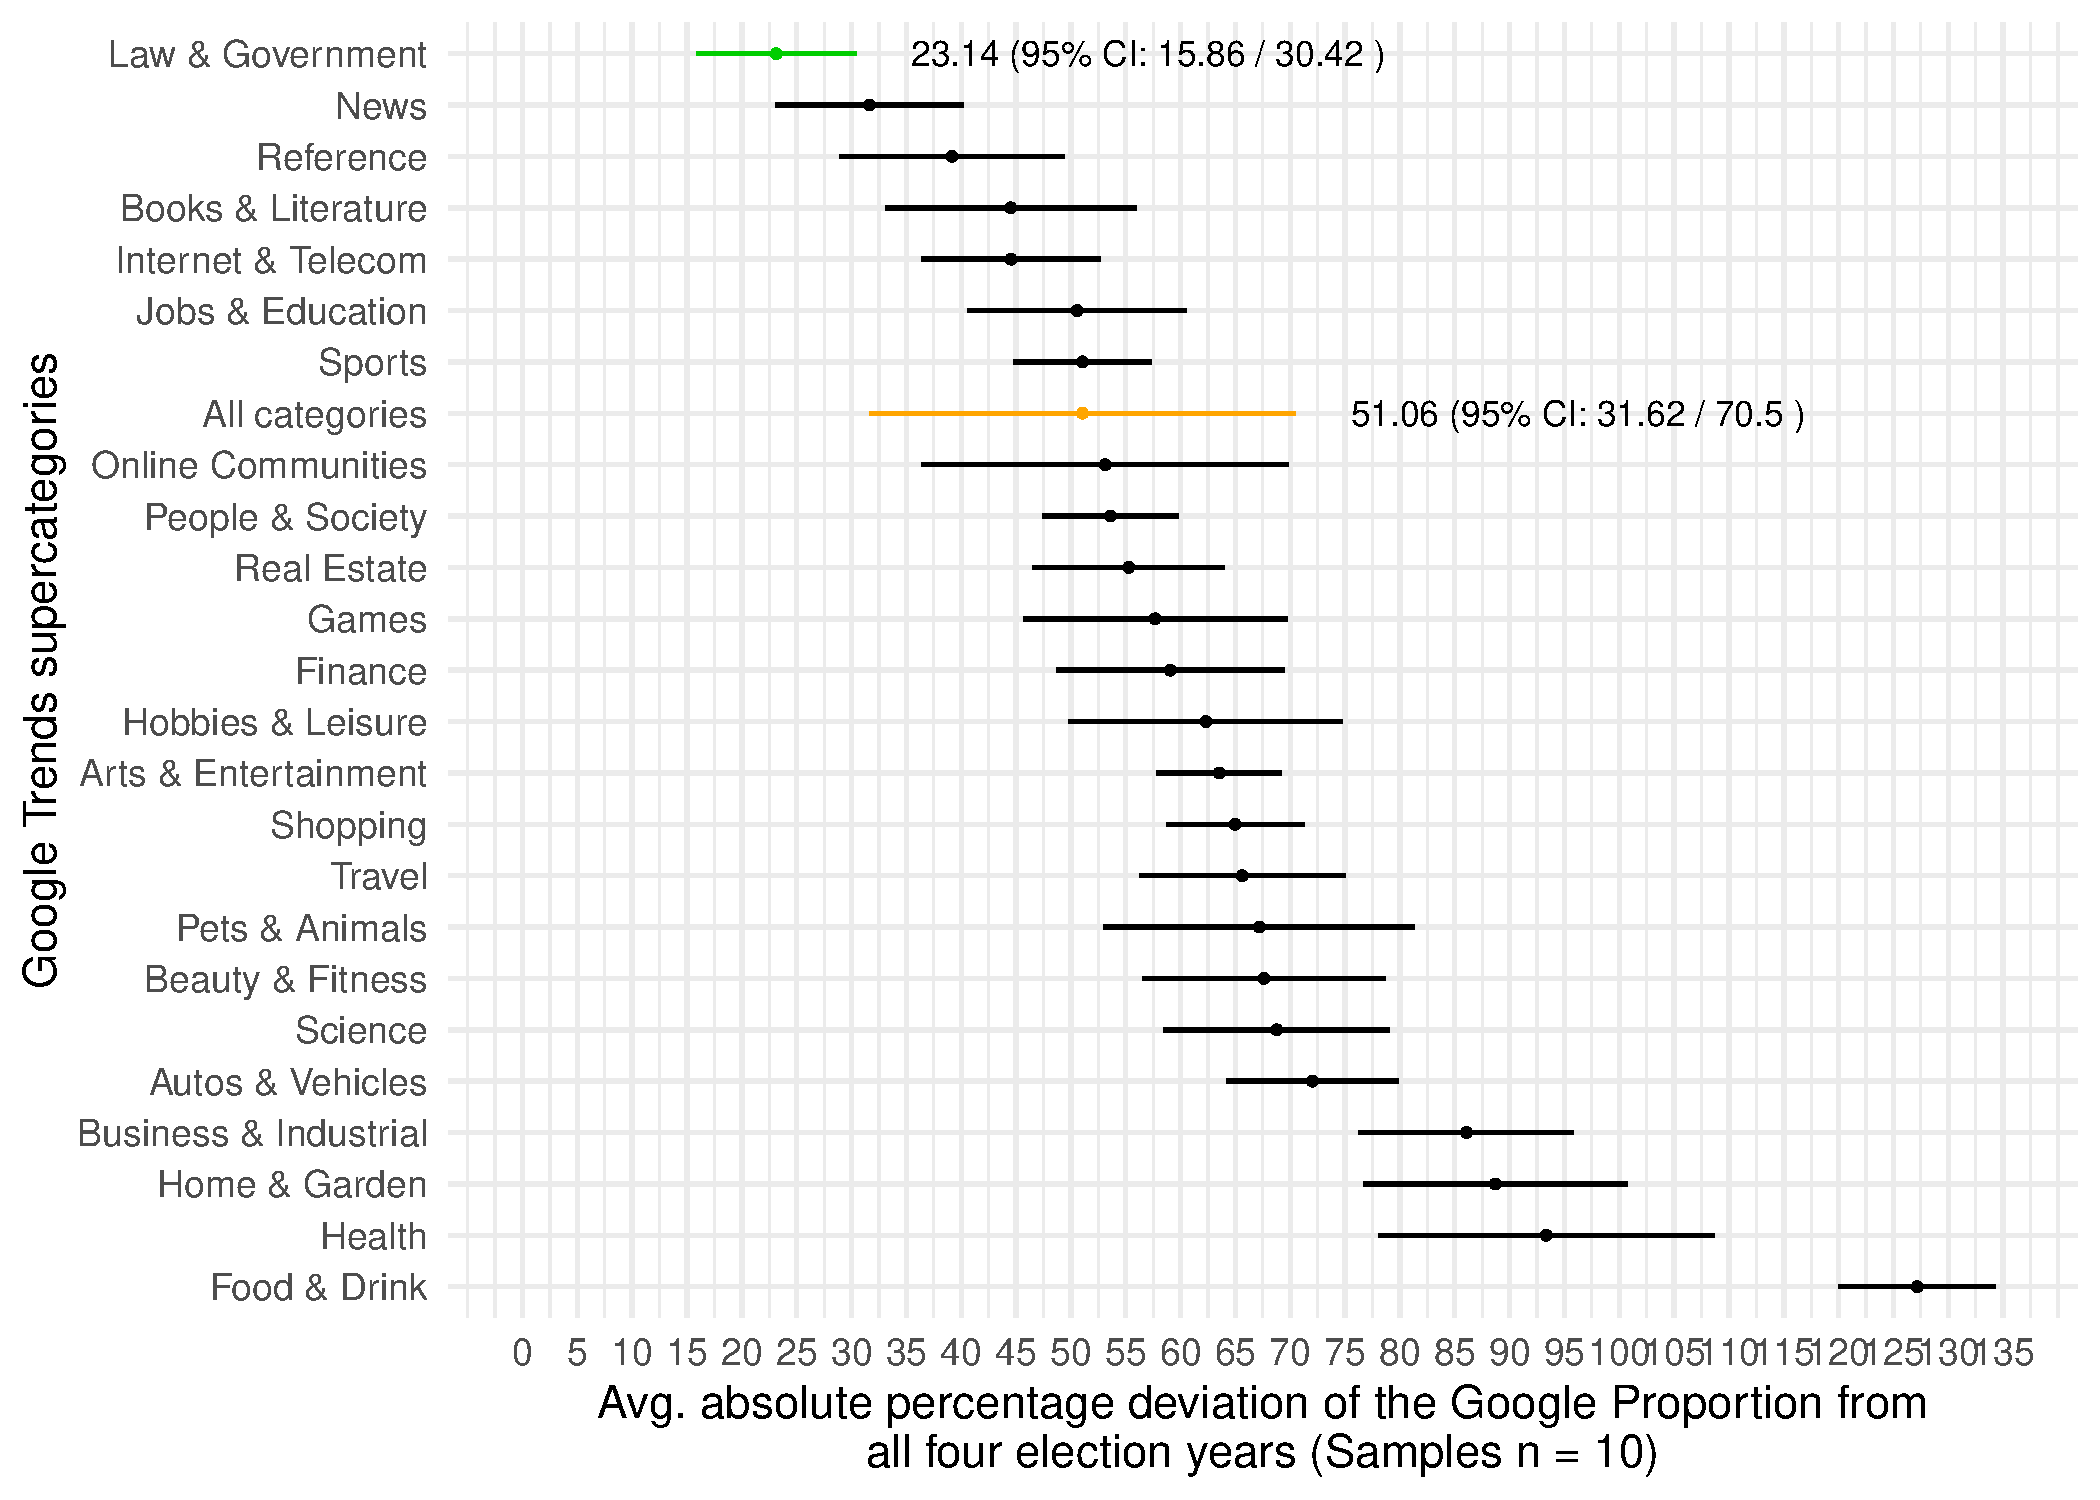
\includegraphics{figures/fig-A1-1.pdf}

}

\end{figure}

Figure~\ref{fig-A2} highlights how the search terms peak for the AfD,
FDP, Grüne and SPD. For the period from 2004 - 2007, for the party ``Die
Linke'' (see Figure~\ref{fig-1}) we found that the abbreviation ``PDS''
and the term ``Linkspartei'' are useful as the best indicators for
predicting elections. The reason is that the party was still called
``Party of Democratic Socialism'' and bore the abbreviation ``PDS''
during those years.

\begin{figure}[H]

\caption{\label{fig-A2}Search terms for other parties}

{\centering 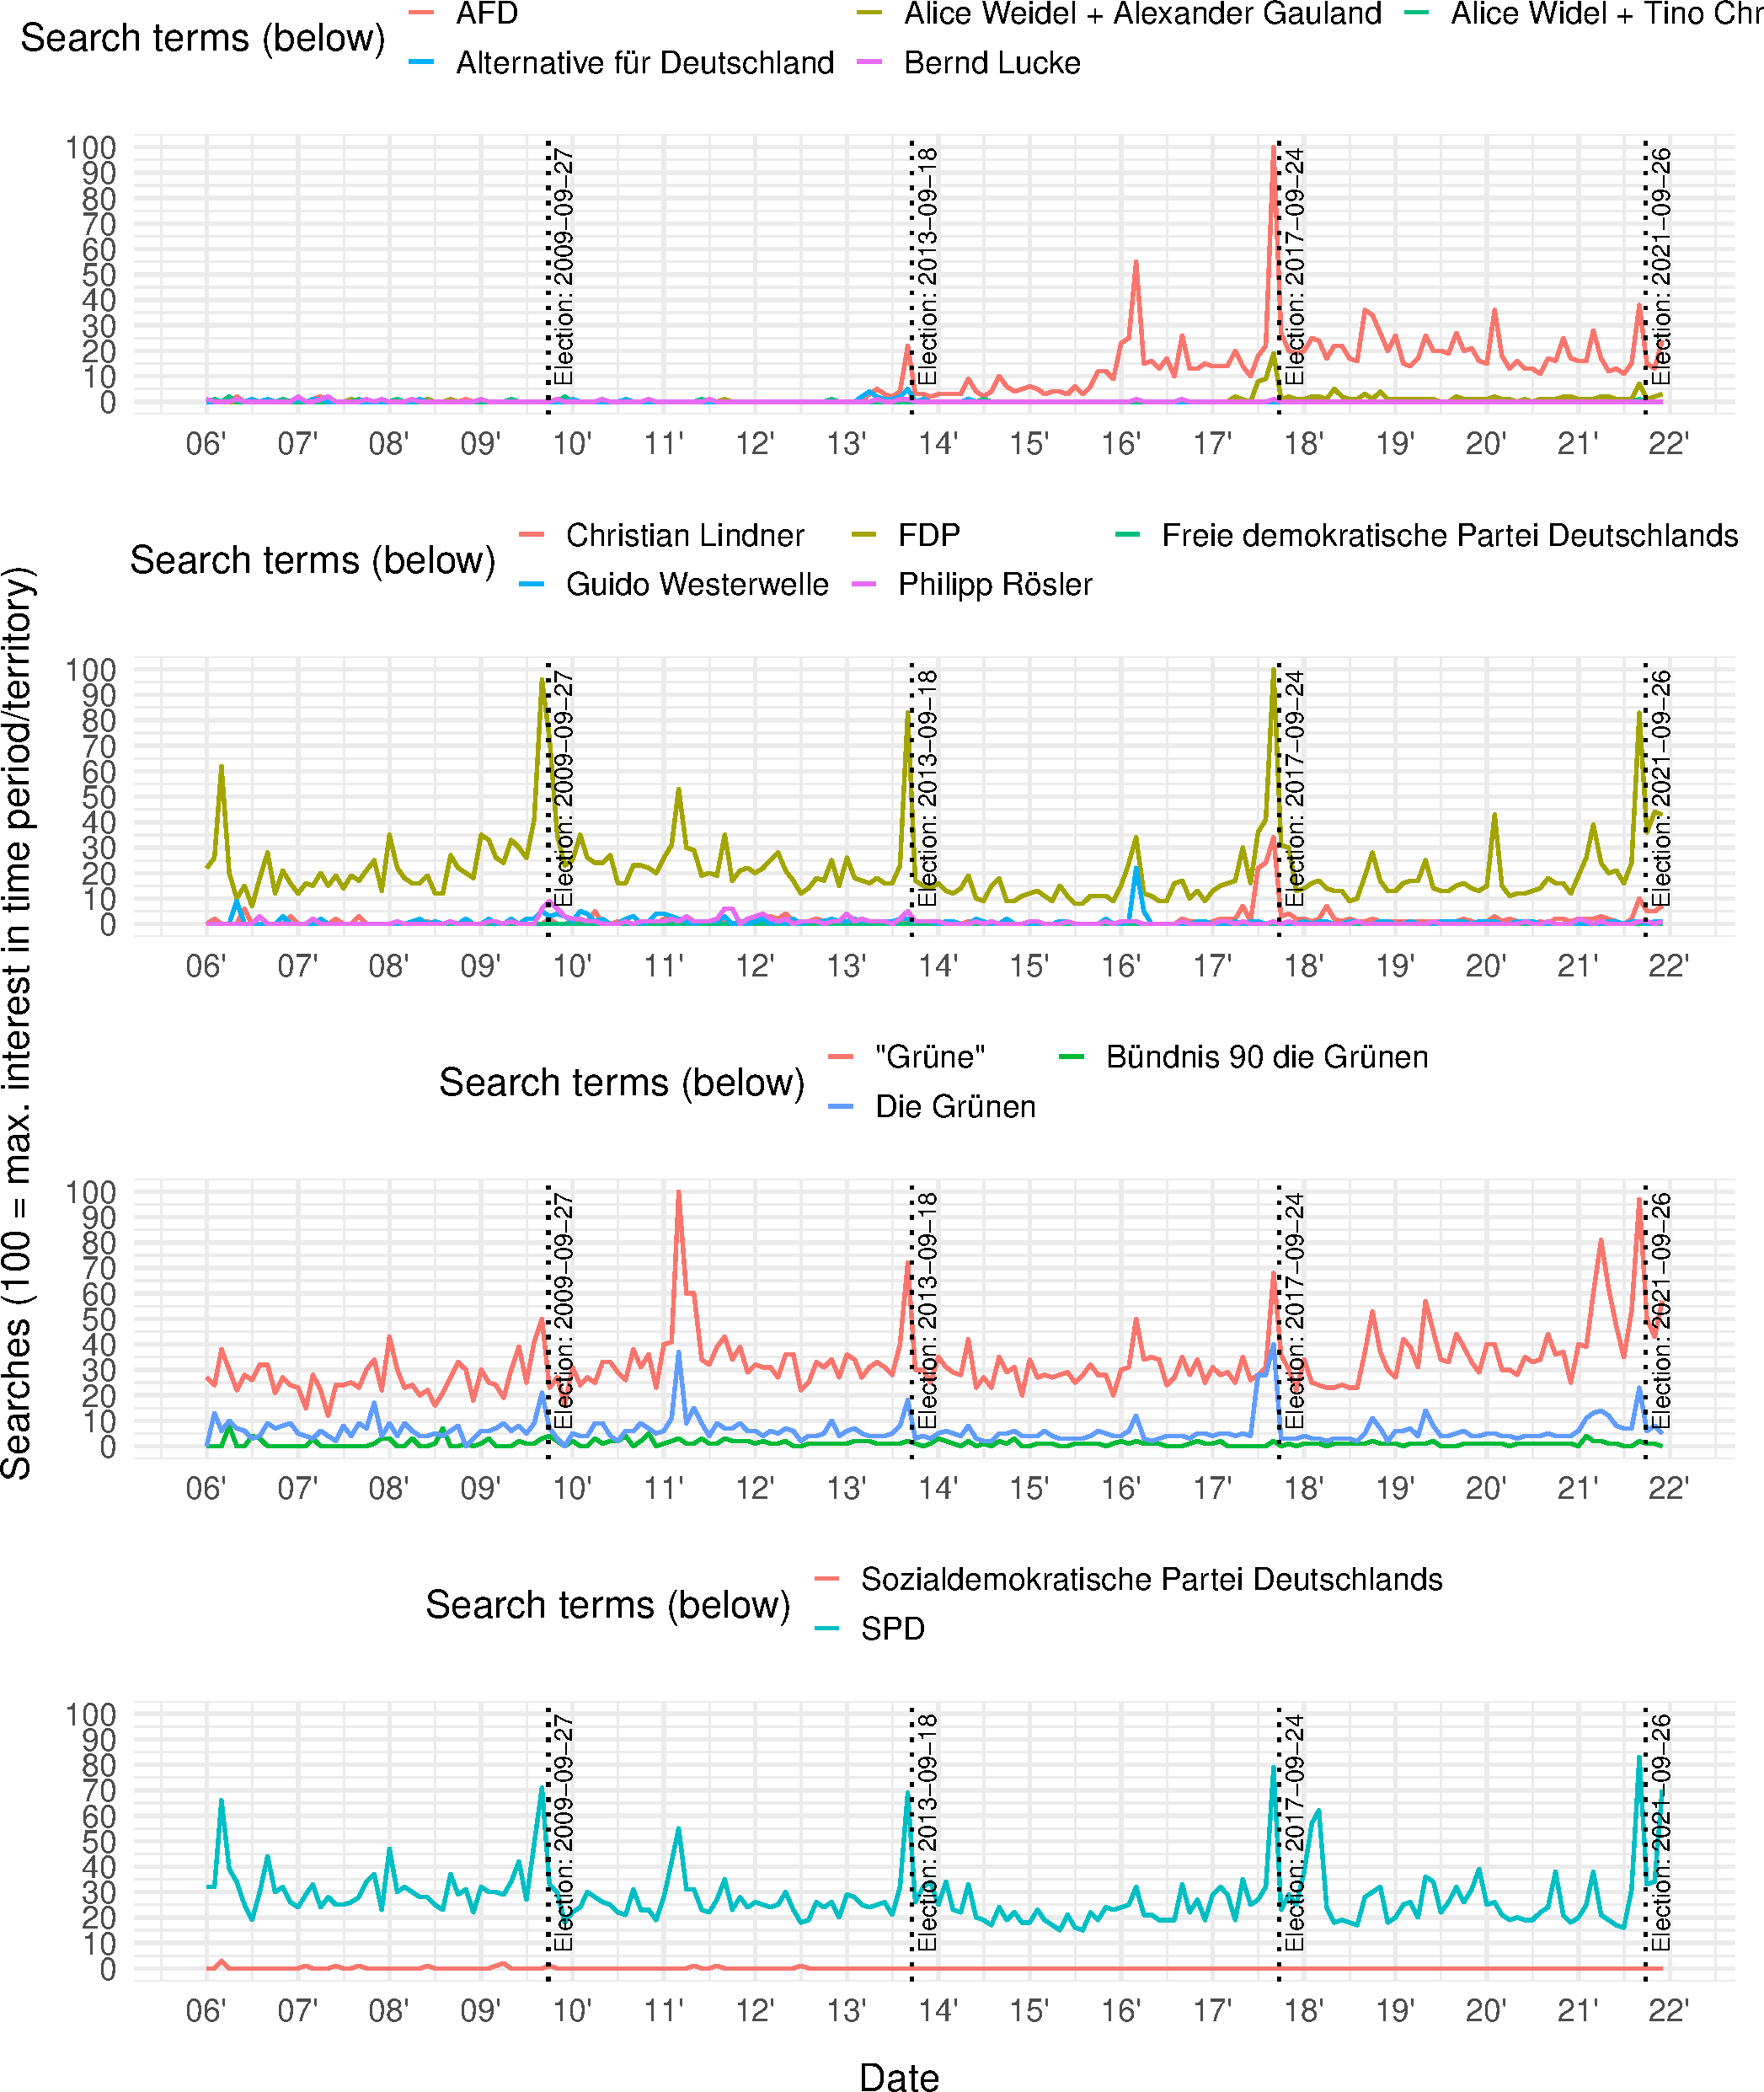
\includegraphics{figures/fig-A2-1.pdf}

}

\end{figure}

\hypertarget{sec-gtsampling}{%
\section{GT data collection and sampling error}\label{sec-gtsampling}}

Table~\ref{tbl-A1} shows the collected datasets across a day that were
different. We collected the data hourly (each collection comprises
several datasets), but Table~\ref{tbl-A1} only shows the collected
samples that are different. Each .Rdata file correspondings to a time
point when we collected the respective GT datasets for the different
search terms. In principle, we could have stored the single datasets
contained in each .Rdata file as .csv-files. But the approach we chose
turned out to be more feasable. As discussed by Raubenheimer et al. (27)
google trends data samples may differ across time. Across the series of
datasets we collected we checked for each .RData file if all the
contained datasets are different as compared to the previously collected
samples. Subsequently, we only used samples for which we identified that
they are not equivalent to the previous ones. For replication purposes
the corresponding .RData files are highlighted in the column ``used'' in
Table~\ref{tbl-A1}. The end time of the respective data collection is
indicated in the ``Time'' column. Each data collection (comprising
several datasets) took around two minutes.

\hypertarget{tbl-A1}{}
\begin{table}
\caption{\label{tbl-A1}Overview datasets across samples that are different }\tabularnewline

\centering\begingroup\fontsize{6}{8}\selectfont

\begin{tabular}{llll}
\toprule
Dataset name & Date & Time & Used\\
\midrule
2022-11-27 11-31-14.RData & 2022-11-27 & 11-31-14 & -\\
2022-11-27 18-31-15.RData & 2022-11-27 & 18-31-15 & -\\
2022-11-28 18-31-13.RData & 2022-11-28 & 18-31-13 & -\\
2022-11-28 21-31-16.RData & 2022-11-28 & 21-31-16 & -\\
2022-11-28 23-31-16.RData & 2022-11-28 & 23-31-16 & -\\
\addlinespace
2022-11-29 09-31-15.RData & 2022-11-29 & 09-31-15 & -\\
2022-11-29 18-31-14.RData & 2022-11-29 & 18-31-14 & -\\
2022-11-29 23-31-15.RData & 2022-11-29 & 23-31-15 & -\\
2022-11-30 00-31-16.RData & 2022-11-30 & 00-31-16 & -\\
2022-11-30 09-31-14.RData & 2022-11-30 & 09-31-14 & -\\
\addlinespace
2022-11-30 10-31-15.RData & 2022-11-30 & 10-31-15 & -\\
2022-11-30 18-31-16.RData & 2022-11-30 & 18-31-16 & -\\
2022-12-01 19-31-13.RData & 2022-12-01 & 19-31-13 & used\\
2022-12-01 23-31-15.RData & 2022-12-01 & 23-31-15 & -\\
2022-12-02 01-31-14.RData & 2022-12-02 & 01-31-14 & used\\
\addlinespace
2022-12-02 03-31-15.RData & 2022-12-02 & 03-31-15 & -\\
2022-12-02 11-31-14.RData & 2022-12-02 & 11-31-14 & -\\
2022-12-02 13-31-16.RData & 2022-12-02 & 13-31-16 & -\\
2022-12-03 01-31-17.RData & 2022-12-03 & 01-31-17 & used\\
2022-12-03 13-31-14.RData & 2022-12-03 & 13-31-14 & -\\
\addlinespace
2022-12-04 00-31-13.RData & 2022-12-04 & 00-31-13 & used\\
2022-12-04 02-31-13.RData & 2022-12-04 & 02-31-13 & -\\
2022-12-05 00-31-16.RData & 2022-12-05 & 00-31-16 & used\\
2022-12-05 01-31-15.RData & 2022-12-05 & 01-31-15 & -\\
2022-12-05 02-31-14.RData & 2022-12-05 & 02-31-14 & -\\
\addlinespace
2022-12-05 21-31-16.RData & 2022-12-05 & 21-31-16 & -\\
2022-12-06 03-31-17.RData & 2022-12-06 & 03-31-17 & used\\
2022-12-06 13-31-14.RData & 2022-12-06 & 13-31-14 & -\\
2022-12-06 15-31-14.RData & 2022-12-06 & 15-31-14 & -\\
2022-12-06 20-31-15.RData & 2022-12-06 & 20-31-15 & -\\
\addlinespace
2022-12-07 04-31-13.RData & 2022-12-07 & 04-31-13 & used\\
2022-12-07 18-31-12.RData & 2022-12-07 & 18-31-12 & -\\
2022-12-07 20-31-13.RData & 2022-12-07 & 20-31-13 & -\\
2022-12-08 18-31-15.RData & 2022-12-08 & 18-31-15 & used\\
2022-12-08 20-31-14.RData & 2022-12-08 & 20-31-14 & -\\
\addlinespace
2022-12-09 06-31-16.RData & 2022-12-09 & 06-31-16 & used\\
2022-12-09 23-31-16.RData & 2022-12-09 & 23-31-16 & -\\
2022-12-10 03-31-13.RData & 2022-12-10 & 03-31-13 & used\\
2022-12-10 07-31-15.RData & 2022-12-10 & 07-31-15 & -\\
2022-12-10 14-31-14.RData & 2022-12-10 & 14-31-14 & -\\
\addlinespace
2022-12-10 19-31-13.RData & 2022-12-10 & 19-31-13 & -\\
2022-12-11 14-31-15.RData & 2022-12-11 & 14-31-15 & -\\
2022-12-12 03-31-14.RData & 2022-12-12 & 03-31-14 & -\\
2022-12-12 07-31-14.RData & 2022-12-12 & 07-31-14 & -\\
2022-12-13 03-31-14.RData & 2022-12-13 & 03-31-14 & -\\
\addlinespace
2022-12-13 07-31-13.RData & 2022-12-13 & 07-31-13 & -\\
2022-12-13 08-31-15.RData & 2022-12-13 & 08-31-15 & -\\
2022-12-13 17-31-13.RData & 2022-12-13 & 17-31-13 & -\\
2022-12-14 09-31-13.RData & 2022-12-14 & 09-31-13 & -\\
2022-12-14 20-31-12.RData & 2022-12-14 & 20-31-12 & -\\
\addlinespace
2022-12-15 08-31-12.RData & 2022-12-15 & 08-31-12 & -\\
2022-12-15 20-31-13.RData & 2022-12-15 & 20-31-13 & -\\
2022-12-16 20-31-15.RData & 2022-12-16 & 20-31-15 & -\\
2022-12-17 02-31-17.RData & 2022-12-17 & 02-31-17 & -\\
2022-12-17 04-31-12.RData & 2022-12-17 & 04-31-12 & -\\
\addlinespace
2022-12-17 20-31-14.RData & 2022-12-17 & 20-31-14 & -\\
2022-12-17 21-31-13.RData & 2022-12-17 & 21-31-13 & -\\
2022-12-18 03-31-15.RData & 2022-12-18 & 03-31-15 & -\\
2022-12-18 04-31-14.RData & 2022-12-18 & 04-31-14 & -\\
2022-12-18 20-31-13.RData & 2022-12-18 & 20-31-13 & -\\
\addlinespace
2022-12-18 21-31-12.RData & 2022-12-18 & 21-31-12 & -\\
2022-12-19 04-31-14.RData & 2022-12-19 & 04-31-14 & -\\
2022-12-19 09-31-13.RData & 2022-12-19 & 09-31-13 & -\\
2022-12-19 14-31-12.RData & 2022-12-19 & 14-31-12 & -\\
2022-12-19 20-31-12.RData & 2022-12-19 & 20-31-12 & -\\
\bottomrule
\end{tabular}
\endgroup{}
\end{table}

Figure~\ref{fig-A3} visualizes exemplarily the variation of the Google
proportion across 10 different samples for the 2021 election. In order
to visualize this variation we used the same samples as used for the
prediction of the 2021 election. The Google proportion was calculated
for each day for each party in each sample. Subsequently, the mean and
confidence intervals were calculated for each day for each party.
Figure~\ref{fig-A3} displays the mean (solid line) and confidence
intervals (shaded area) across days and parties. We find that the
variability accross samples is relatively low.

\begin{figure}[H]

\caption{\label{fig-A3}Sampling error variation for the 2021 election}

{\centering 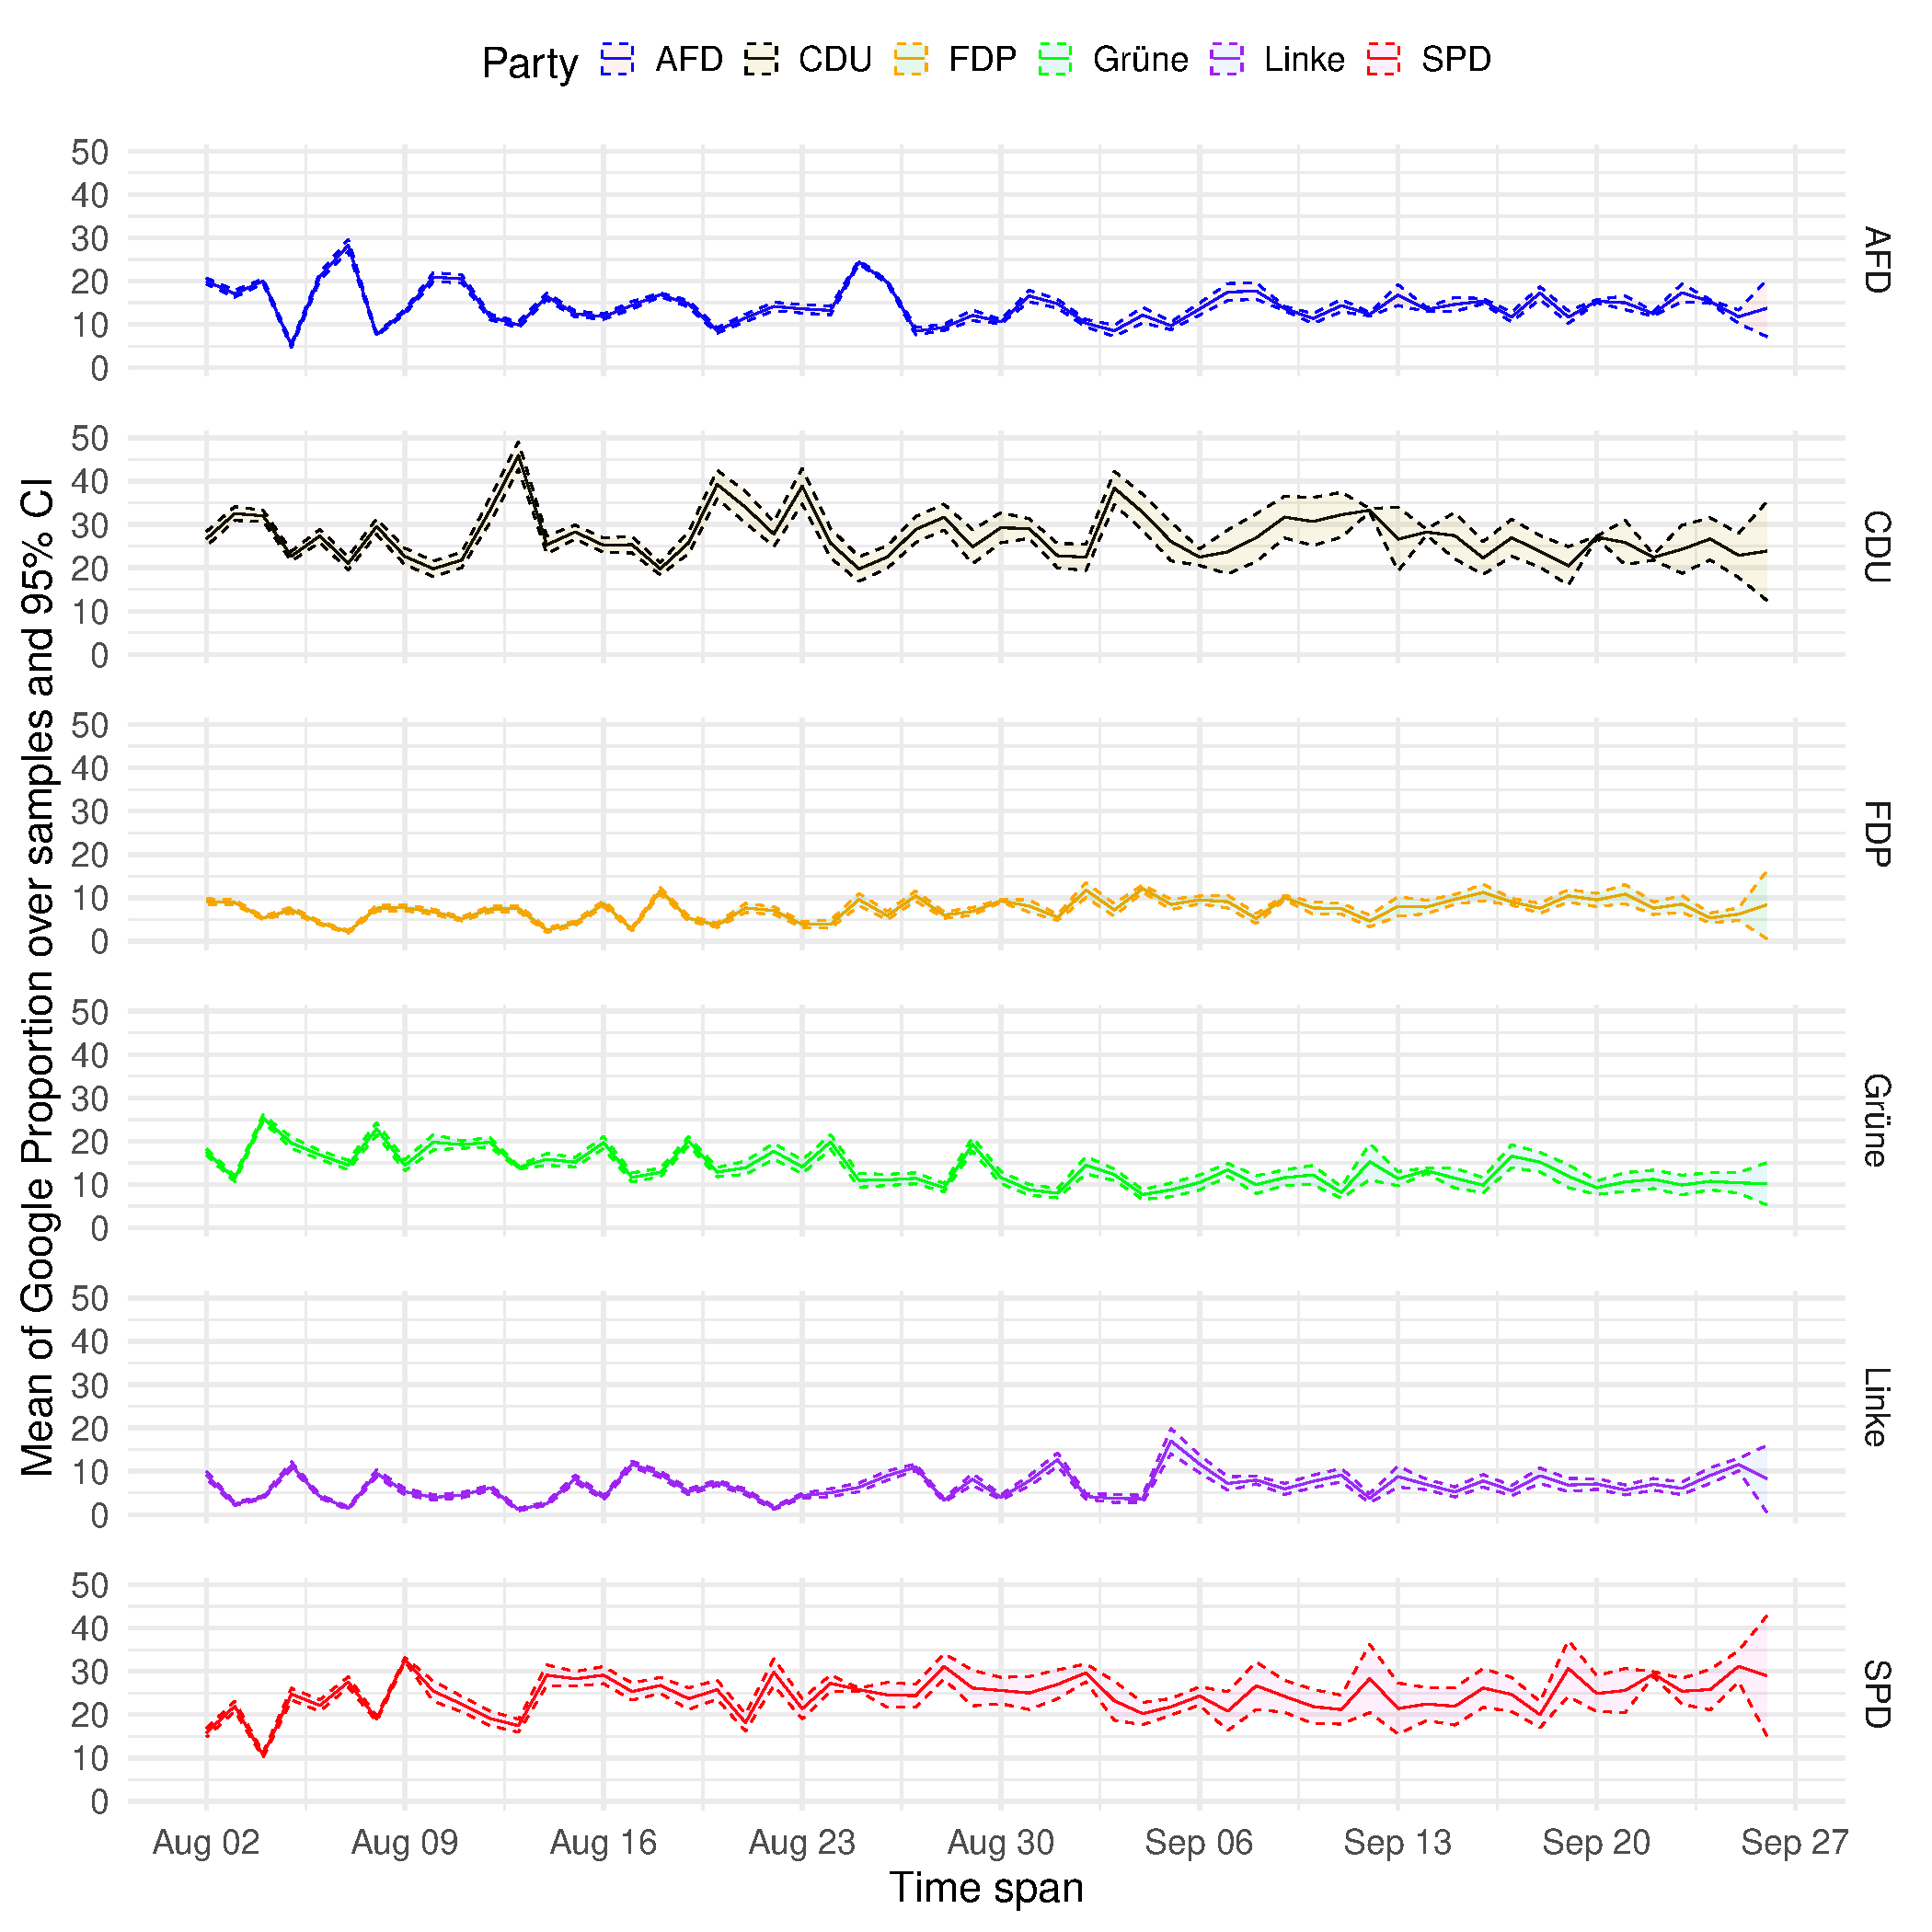
\includegraphics{figures/fig-A3-1.pdf}

}

\end{figure}

\hypertarget{models-and-weighting-methods}{%
\section{Models and weighting
methods}\label{models-and-weighting-methods}}

Challenges when calculating the weighting factor for class MC3: In
single cases, especially for small intervals, it can occur that the mean
Google proportion for single parties within an interval is 0 when
calculating the weighting factor. If the poll for weighting were then
divided by the mean Google proportion, the weighting factor for that
party would be 0 and the data to be weighted would also be 0. To
circumvent this problem, the 0 of this party in the Google proportion is
replaced by the value the party has in the poll used for weighting and
when this poll is divided by the Google proportion to calculate the
weighting factor, the weighting factor for this party is not 0 but 1,
which means that no weighting takes place for this party and solely the
Google Proportion of this party is used. A further issue that had to be
circumvented is that the 2013 polls do not consistently include a value
for the AFD party, as this party was newly founded in 2013. The
procedure is therefore to ignore the calculation of the weighting factor
and assign a weighting value of 1 in these cases to the AFD, so that no
weighting takes place if the entry is missing and only the Google
Proportion is used.

\hypertarget{further-results}{%
\section{Further results}\label{further-results}}

\hypertarget{comparing-predictions-across-gt-data-windows-across-parties-other-elections-and-widths}{%
\subsection{Comparing predictions across GT data windows, across
parties: Other elections and
widths}\label{comparing-predictions-across-gt-data-windows-across-parties-other-elections-and-widths}}

Figure~\ref{fig-A4} is the same as Figure~\ref{fig-4} only that we added
additional data windows that vary in terms of width (21, 42, 56, 70
days). Generally, our conclusions from Figure~\ref{fig-4} do not change
once we add additional intervals in Figure~\ref{fig-A4}.
Figure~\ref{fig-A5} provides results for the other three elections
(2009, 2013, 2017). Figure~\ref{fig-A5} highlights that there is
considerable differences across elections.

\begin{figure}[H]

\caption{\label{fig-A4}Accuracy of GT predictions for different parties
and party shares across data windows (more intervals)}

{\centering 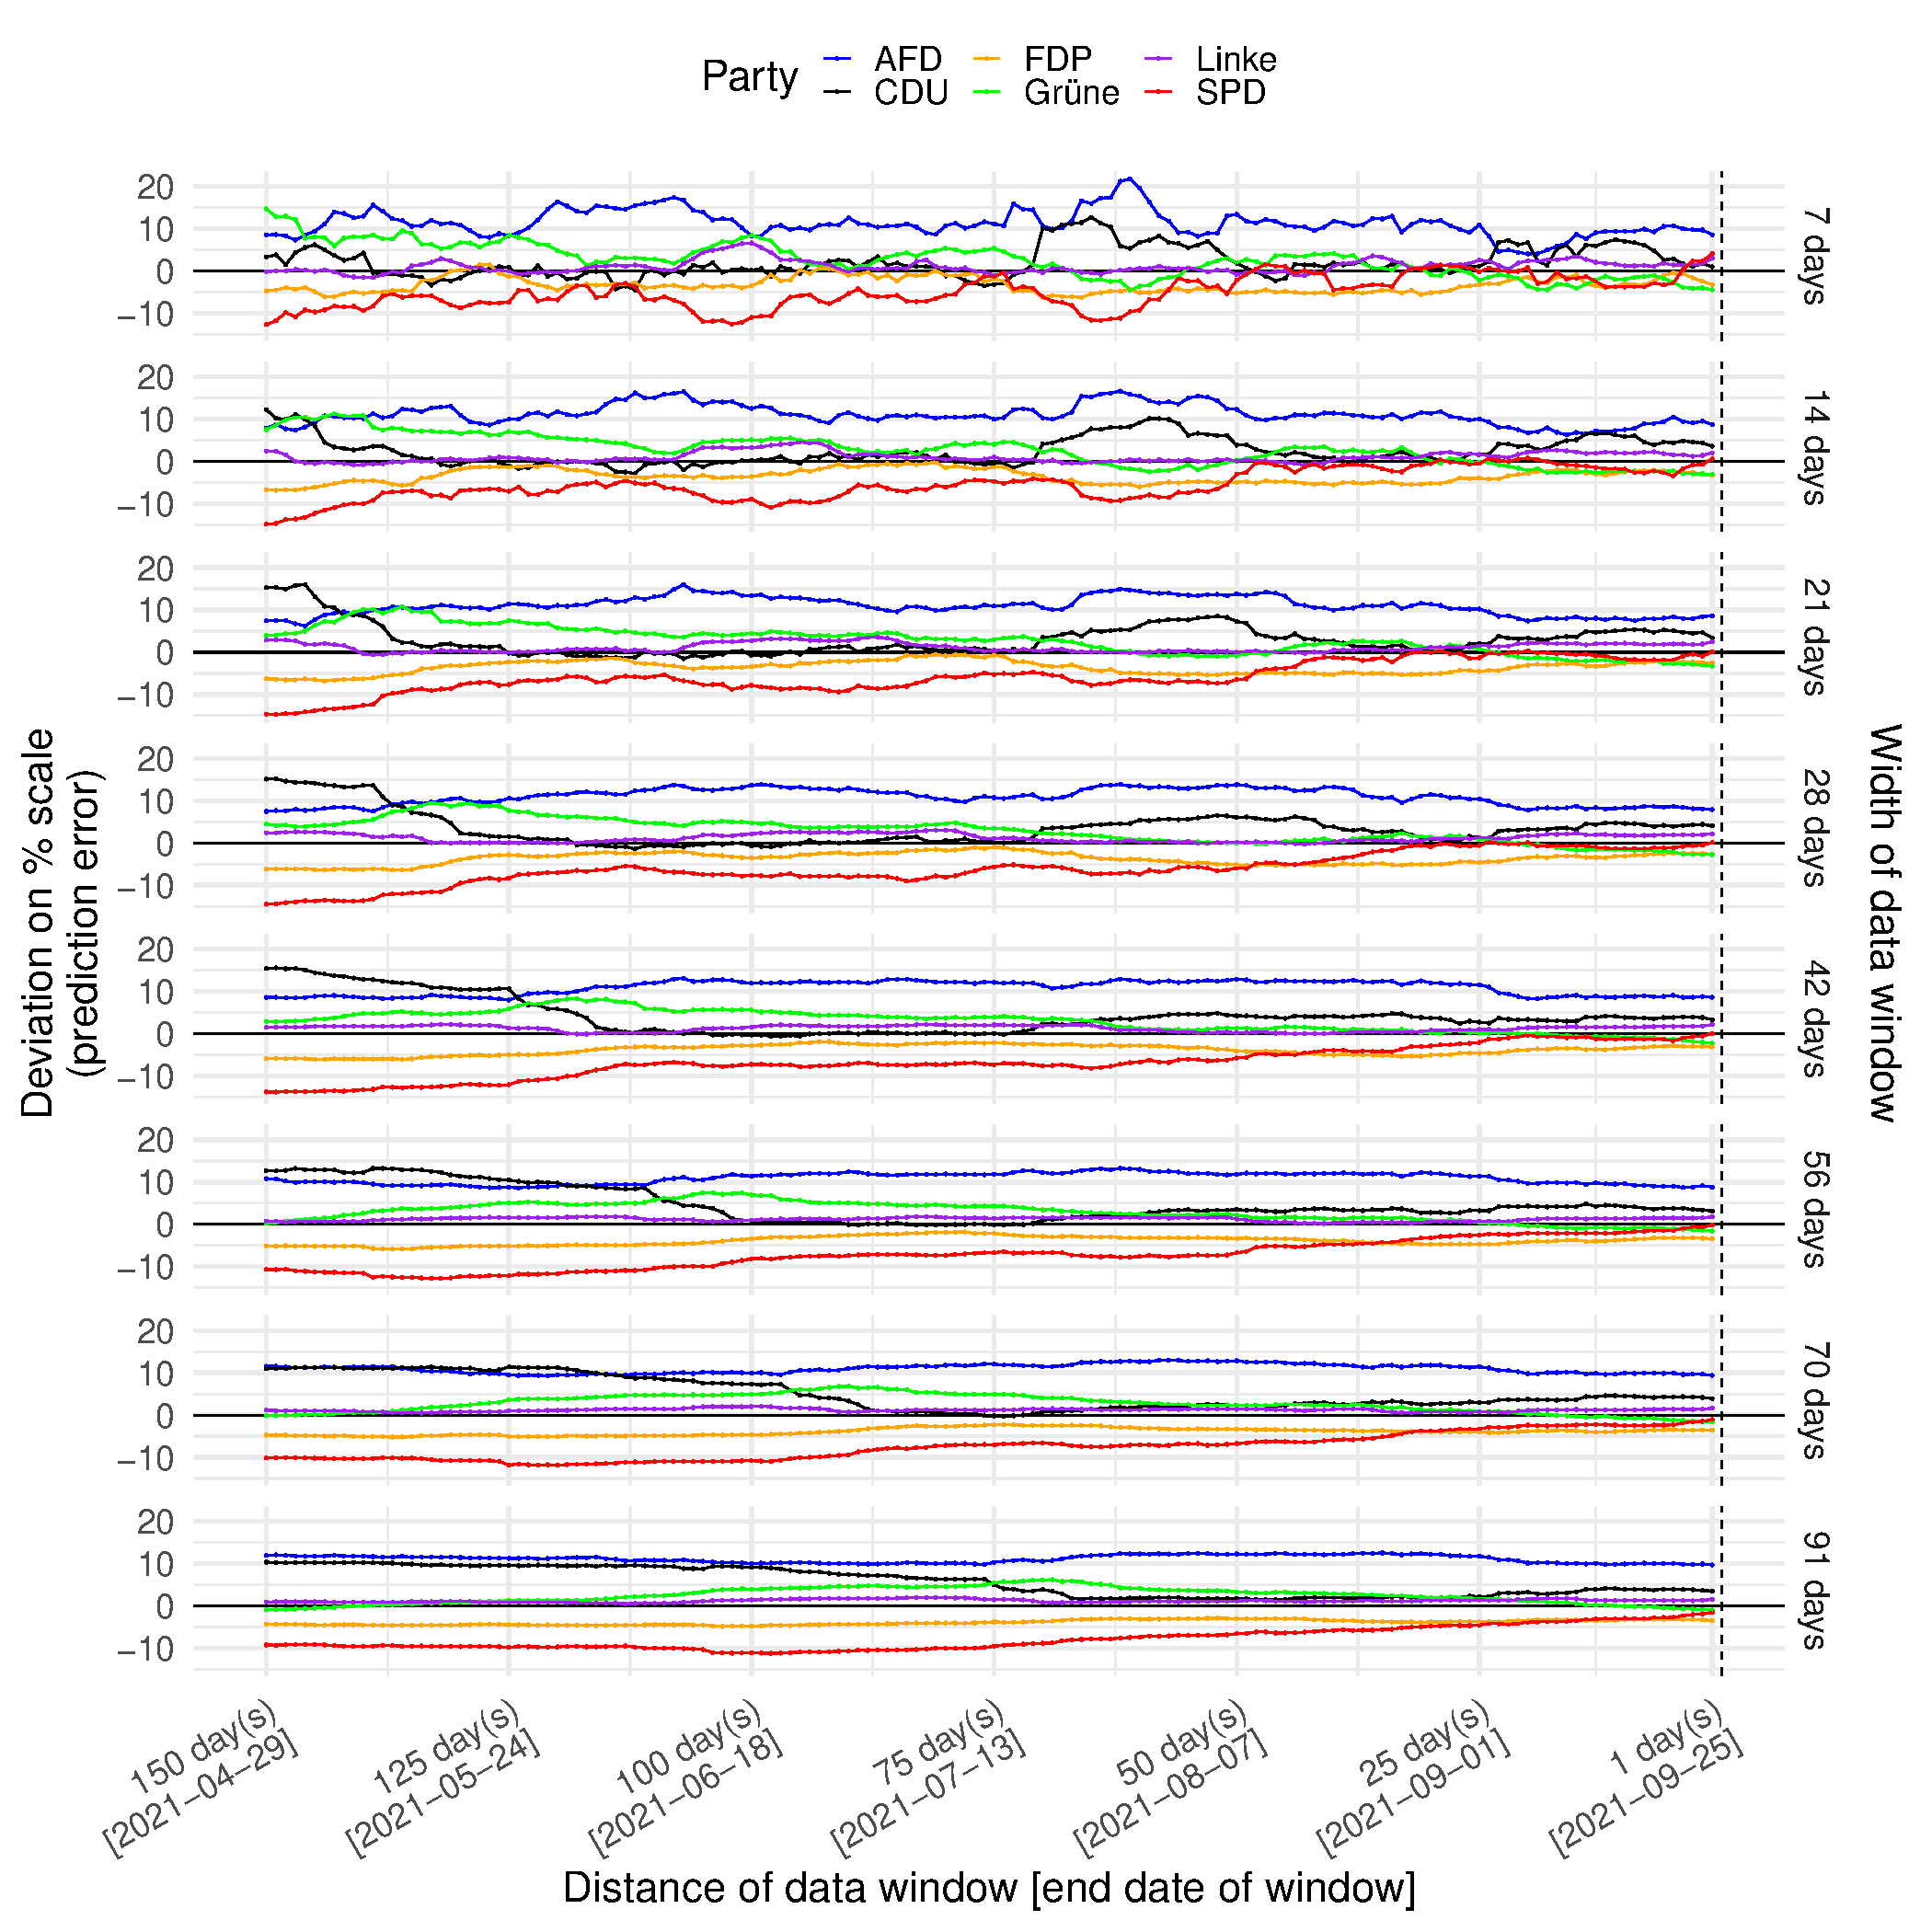
\includegraphics{figures/fig-A4-1.pdf}

}

\end{figure}

\begin{figure}[H]

\caption{\label{fig-A5}Accuracy of GT predictions for different parties
and party shares across data windows (more intervals, elections)}

{\centering 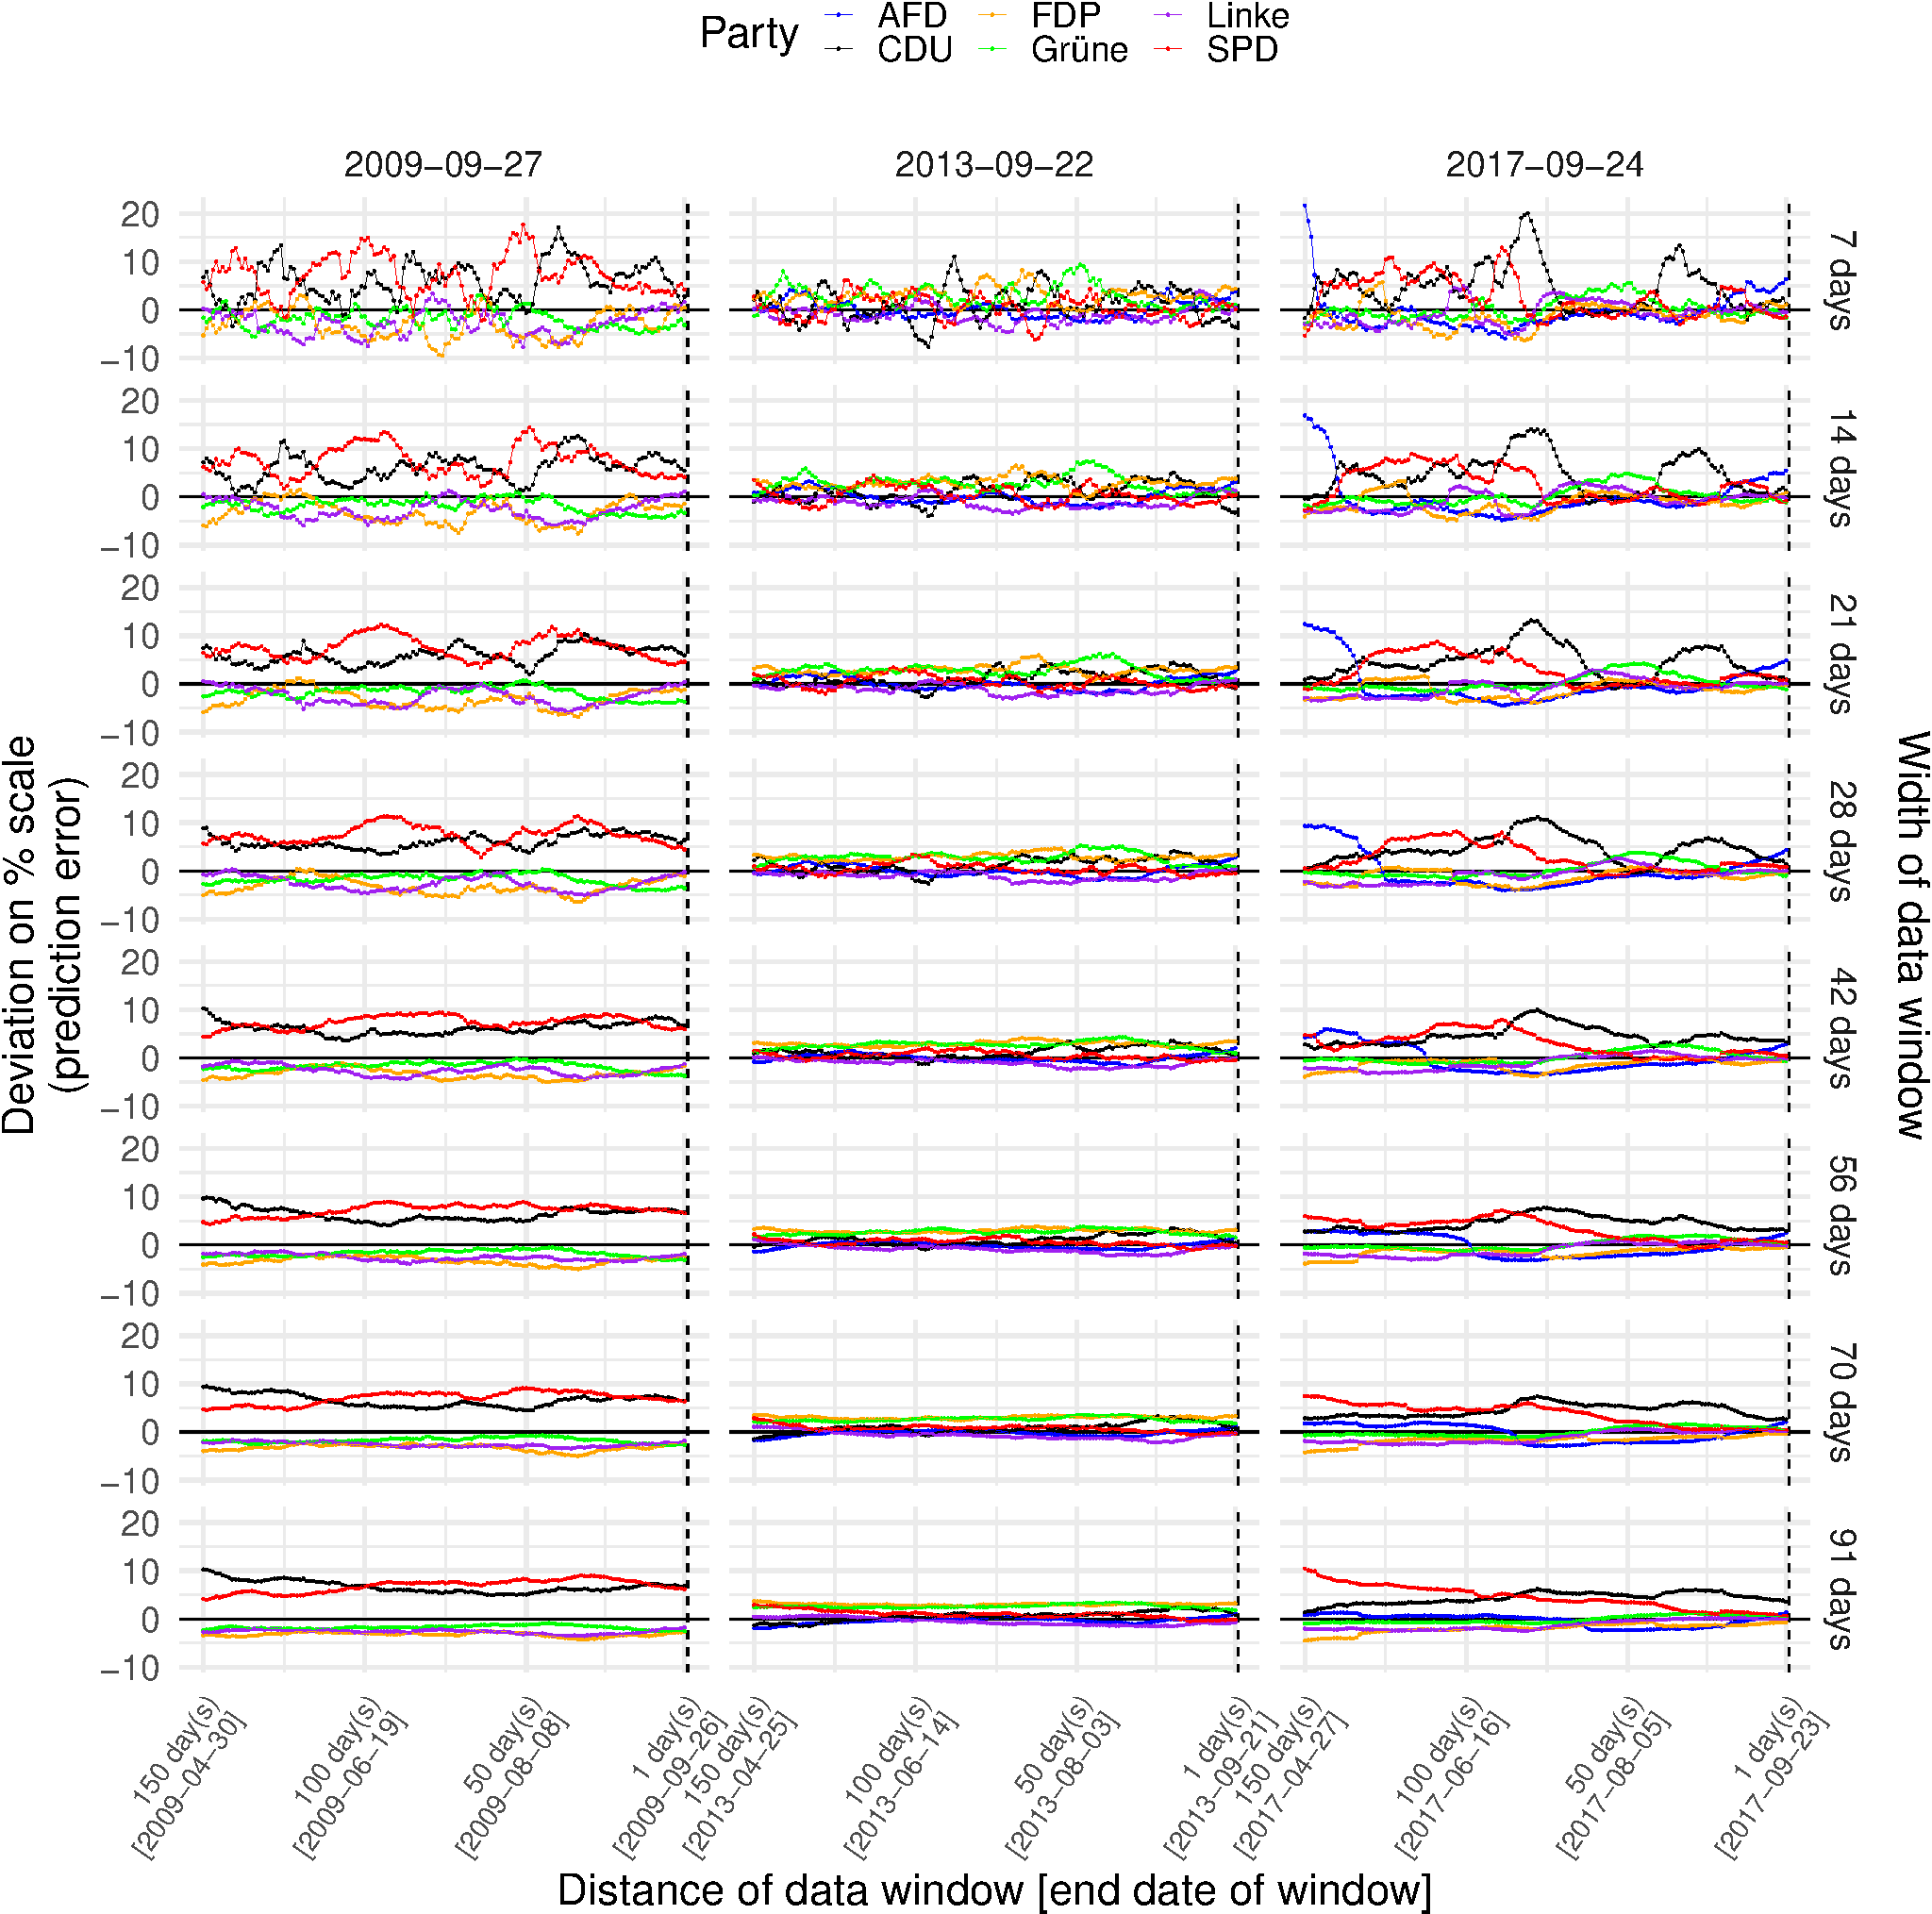
\includegraphics{figures/fig-A5-1.pdf}

}

\end{figure}

Table~\ref{tbl-A2} models the prediction accuracy as a function of the
data window's distance to the election. Thereby, the width of the data
window is held constant at 14 days.

\hypertarget{tbl-A2}{}
\begin{table}[!htbp] \centering 
  \caption{\label{tbl-A2}Prediction accuracy as a function of distance days } 
  \label{} 
\scriptsize 
\begin{tabular}{@{\extracolsep{5pt}}lccccc} 
\\[-1.8ex]\hline 
\hline \\[-1.8ex] 
 & \multicolumn{5}{c}{Dependent variable: Average absolute deviations} \\ 
\cline{2-6} 
 & \shortstack{M1 \\ (all elections)} & \shortstack{M2 \\ (2009-09-27)} & \shortstack{M3 \\ (2013-09-22)} & \shortstack{M4 \\ (2017-09-24)} & \shortstack{M5 \\ (2021-09-26)} \\ 
\hline \\[-1.8ex] 
 Distance (days) & $-$0.007$^{***}$ & 0.007$^{***}$ & 0.003$^{**}$ & $-$0.018$^{***}$ & $-$0.019$^{***}$ \\ 
  & (0.001) & (0.003) & (0.001) & (0.002) & (0.003) \\ 
  & & & & & \\ 
 Constant & 3.922$^{***}$ & 3.765$^{***}$ & 1.770$^{***}$ & 4.035$^{***}$ & 6.094$^{***}$ \\ 
  & (0.107) & (0.226) & (0.089) & (0.173) & (0.263) \\ 
  & & & & & \\ 
\hline \\[-1.8ex] 
Observations & 3,450 & 750 & 900 & 900 & 900 \\ 
R$^{2}$ & 0.010 & 0.010 & 0.007 & 0.080 & 0.042 \\ 
Adjusted R$^{2}$ & 0.010 & 0.008 & 0.005 & 0.079 & 0.041 \\ 
\hline 
\hline \\[-1.8ex] 
\textit{Note:}  & \multicolumn{5}{r}{$^{*}$p$<$0.1; $^{**}$p$<$0.05; $^{***}$p$<$0.01} \\ 
\end{tabular} 
\end{table}

\hypertarget{sec-comparing-model-classes-other}{%
\subsection{Comparing predictions across model classes: Other elections
and data window widths}\label{sec-comparing-model-classes-other}}

Figure~\ref{fig-A6}, Figure~\ref{fig-A7} and Figure~\ref{fig-A8}
replicate Figure~\ref{fig-5} for other elections.

\begin{figure}[H]

\caption{\label{fig-A6}Accuracy of predictions across model classes for
2009 election}

{\centering 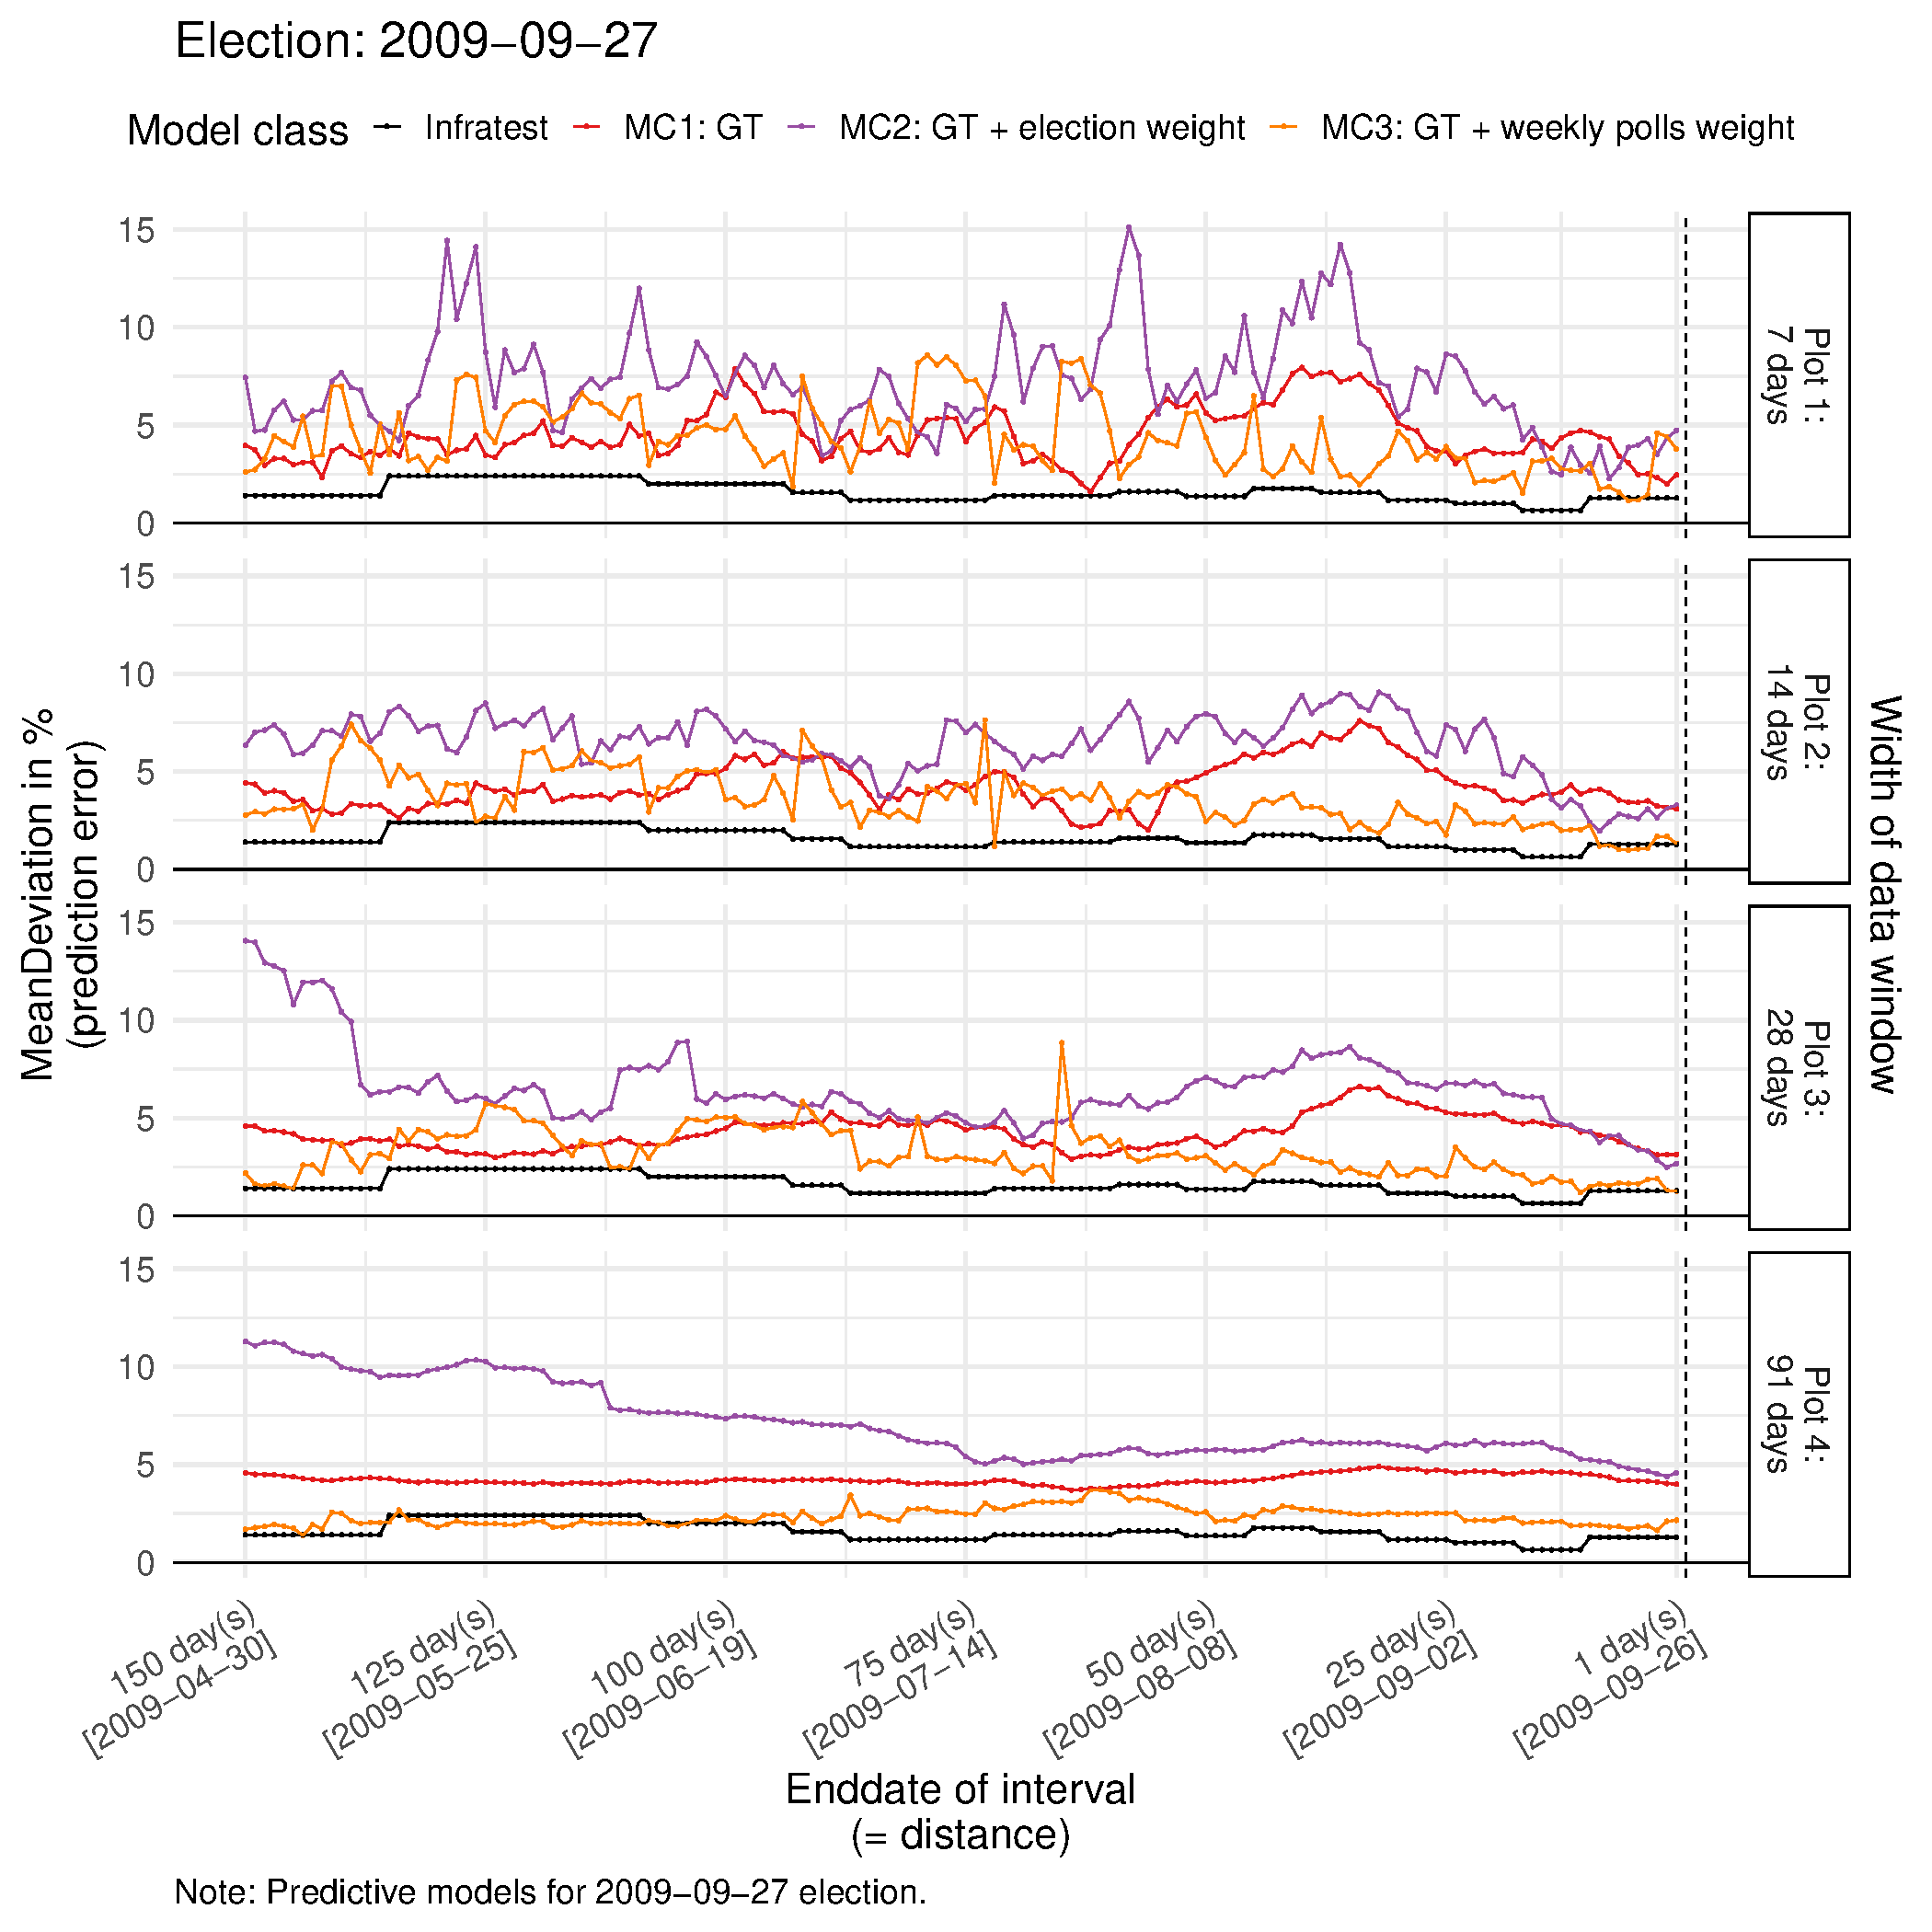
\includegraphics{figures/fig-A6-1.pdf}

}

\end{figure}

\begin{figure}[H]

\caption{\label{fig-A7}Accuracy of predictions across model classes for
2013 election}

{\centering 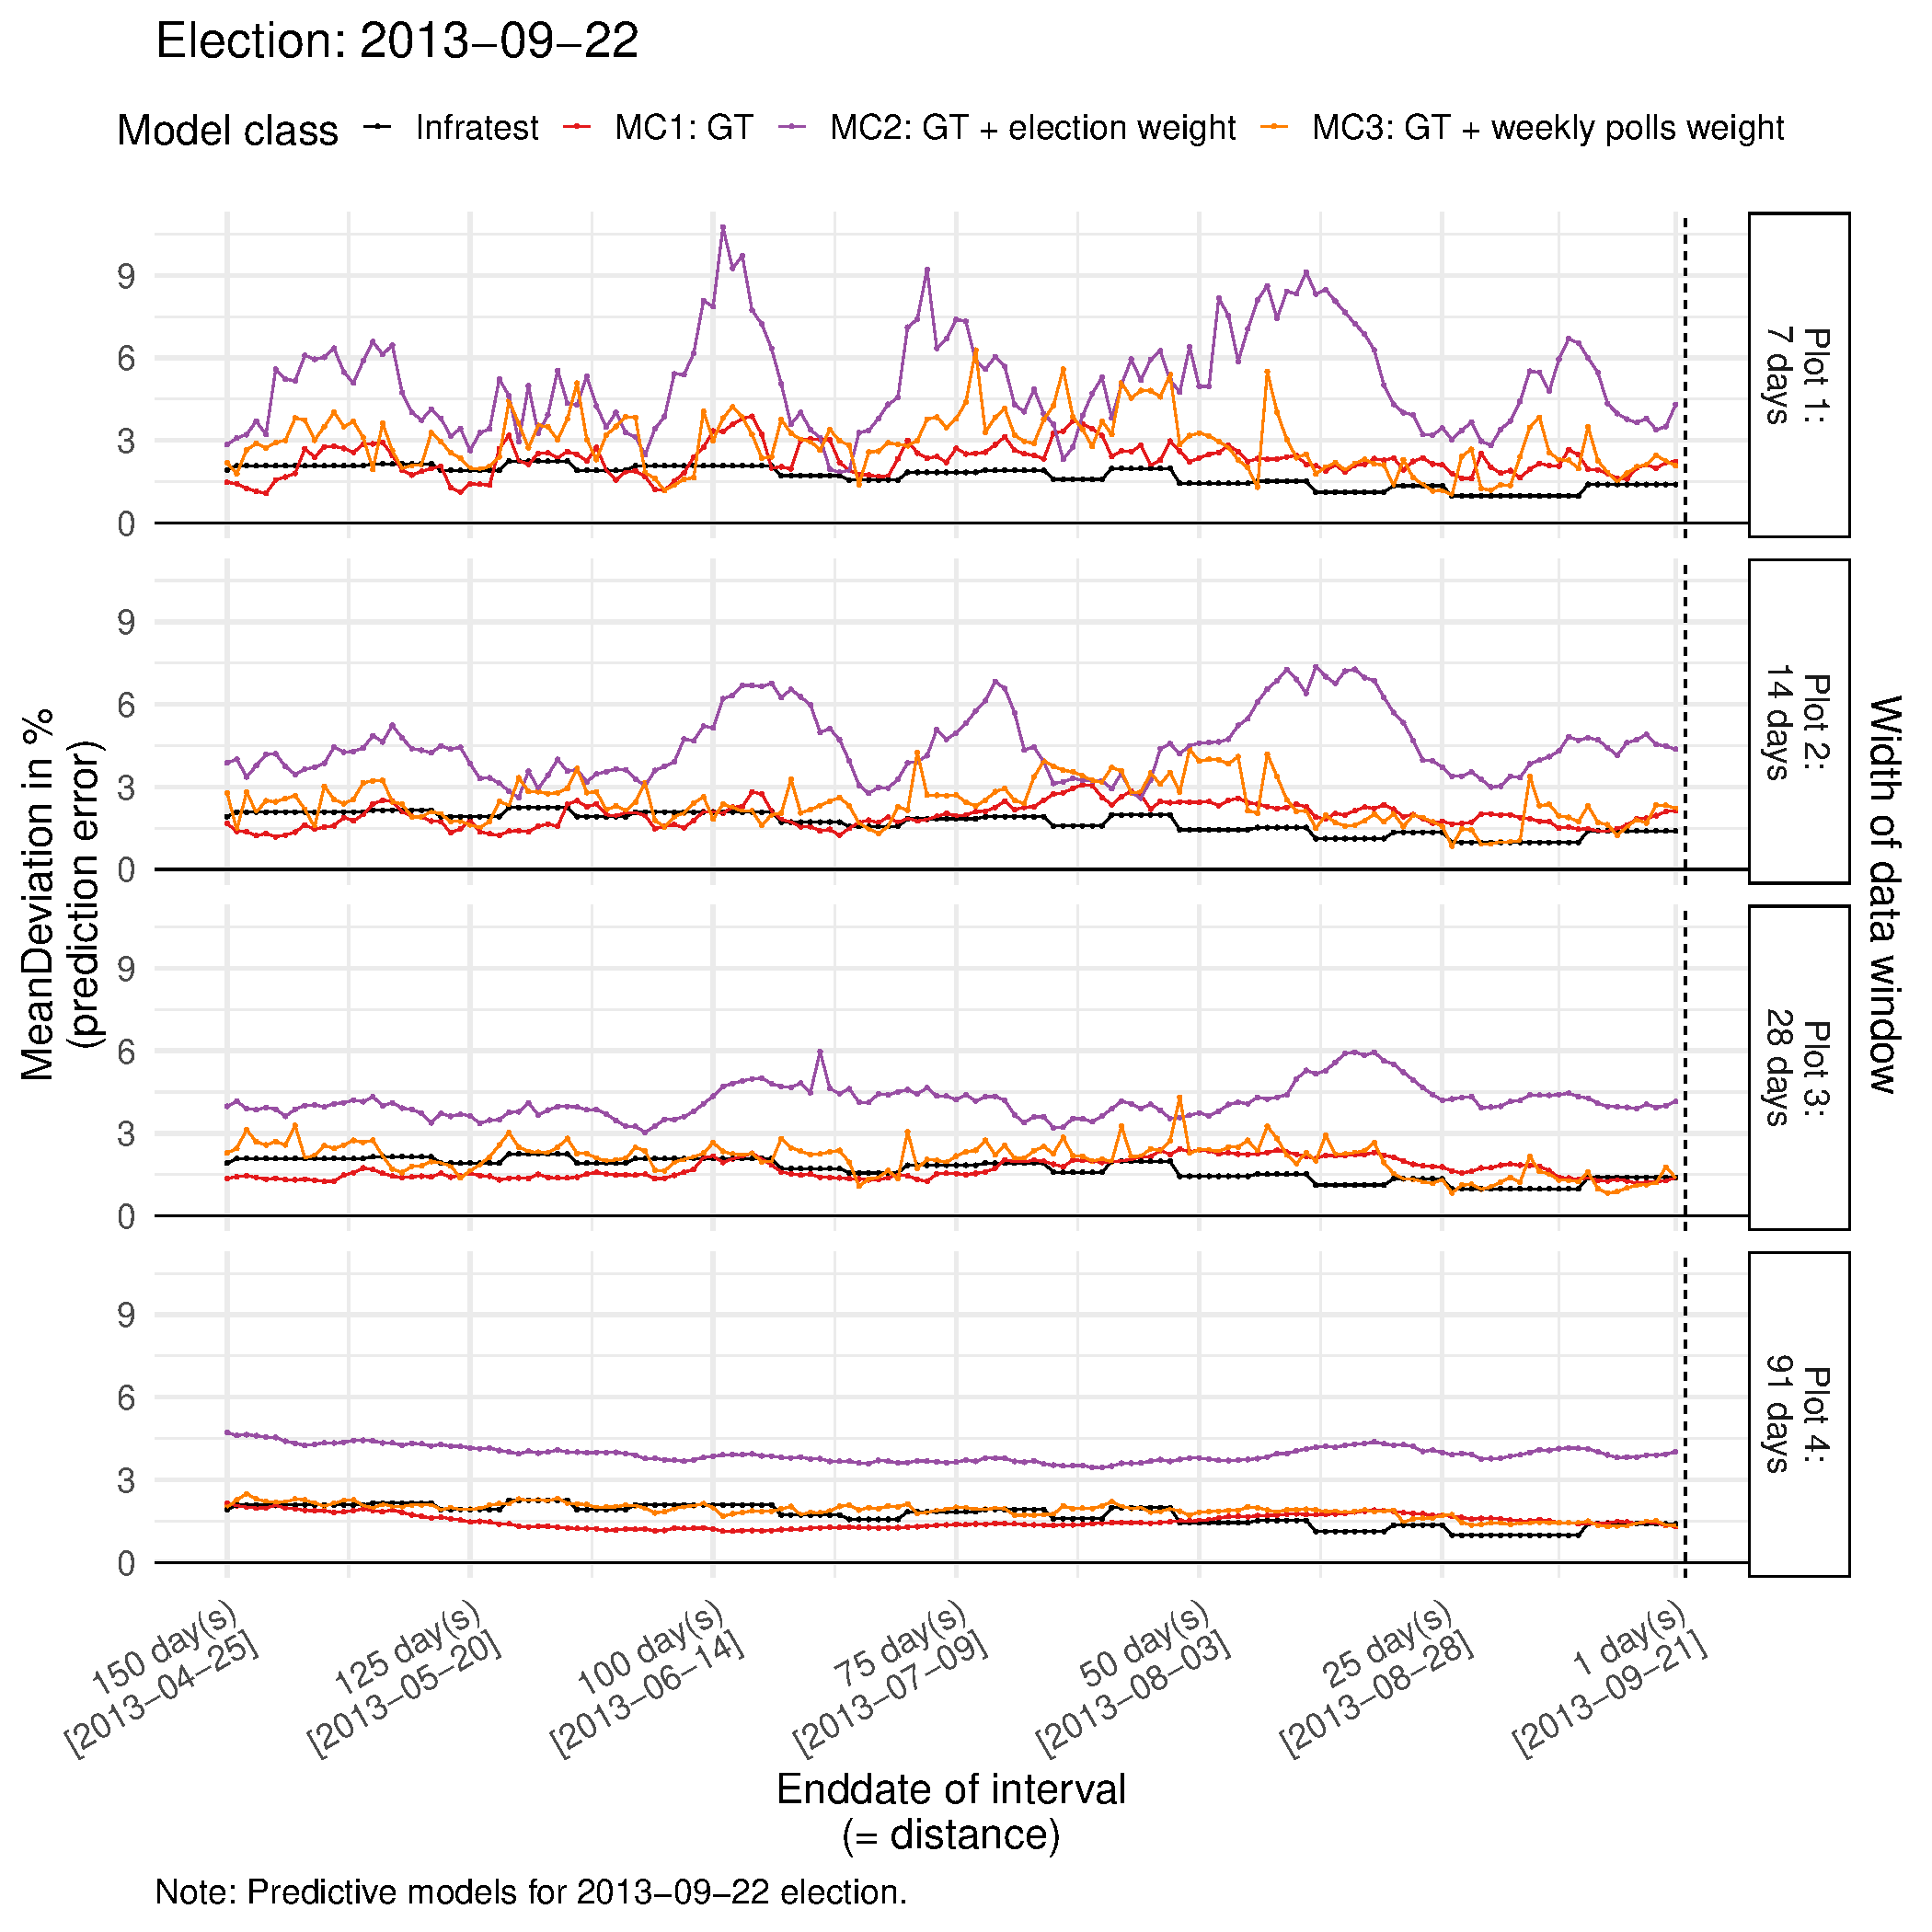
\includegraphics{figures/fig-A7-1.pdf}

}

\end{figure}

\begin{figure}[H]

\caption{\label{fig-A8}Accuracy of predictions across model classes for
2017 election}

{\centering 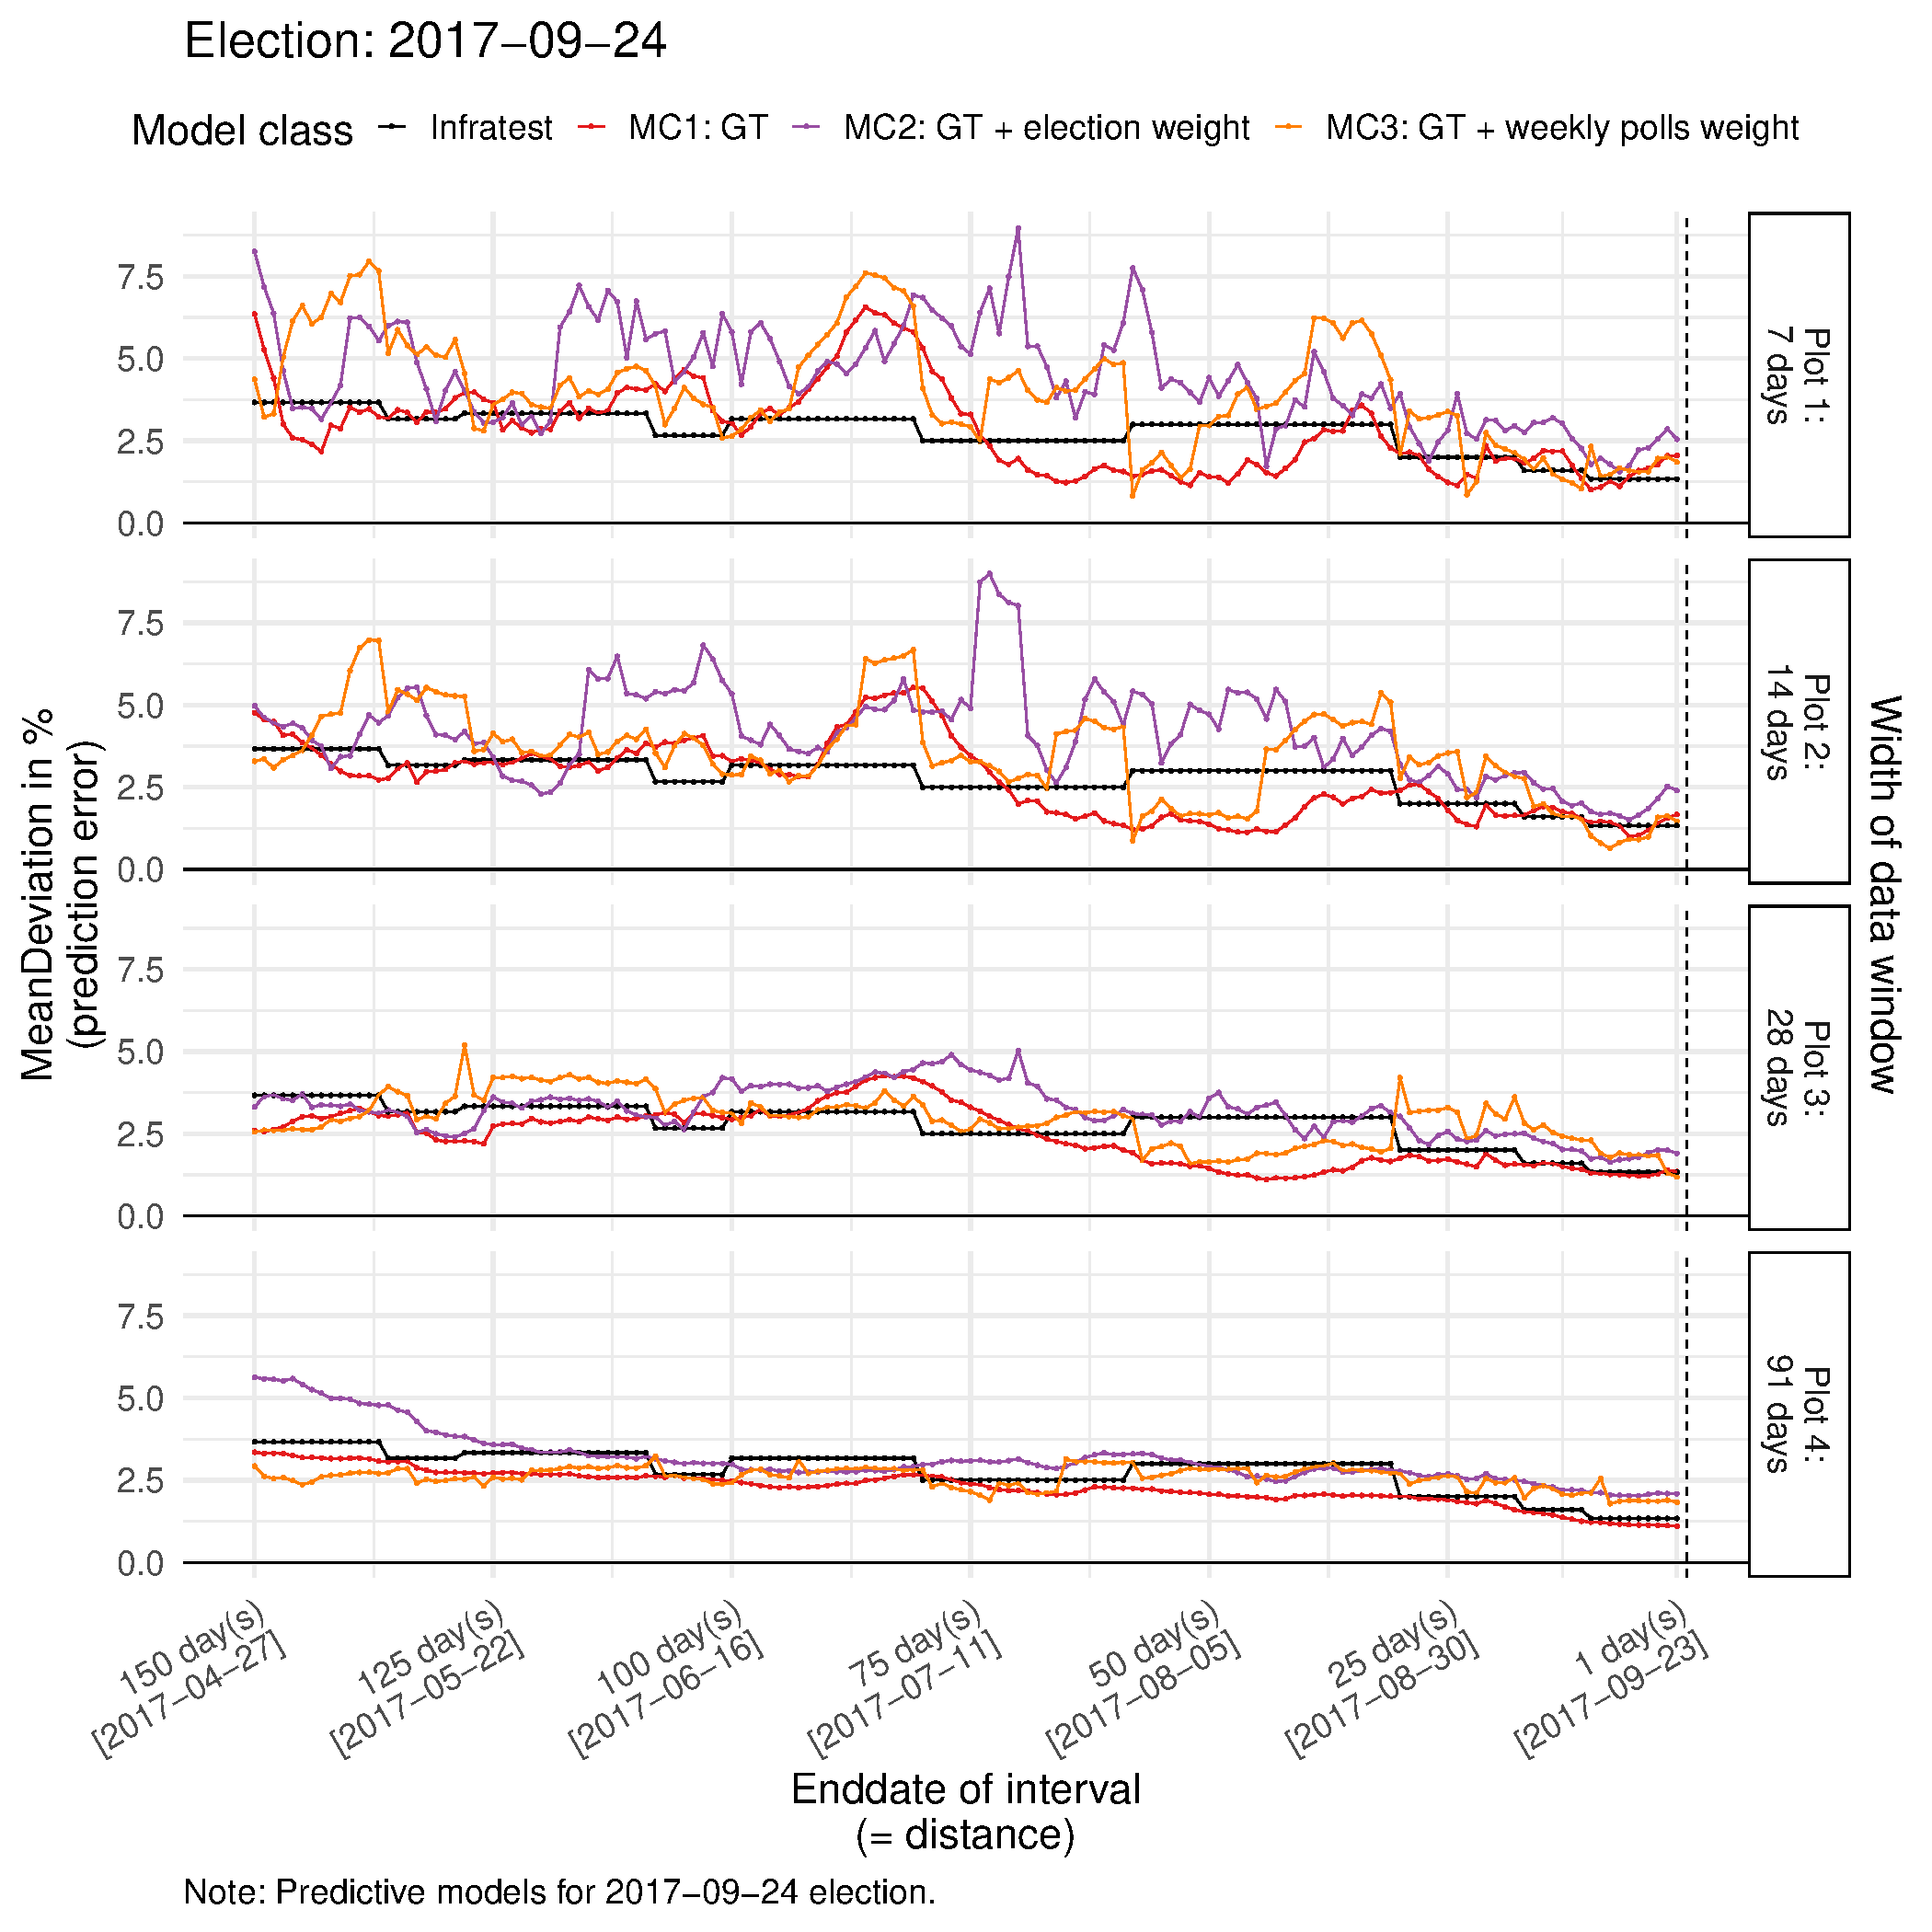
\includegraphics{figures/fig-A8-1.pdf}

}

\end{figure}

\hypertarget{replicating-analyses-across-more-elections}{%
\section{Replicating analyses across more
elections}\label{replicating-analyses-across-more-elections}}

Figure~\ref{fig-A9} replicates Figure~\ref{fig-5} for other elections
side-by-side.

\begin{figure}[H]

\caption{\label{fig-A9}Comparison across elections}

{\centering 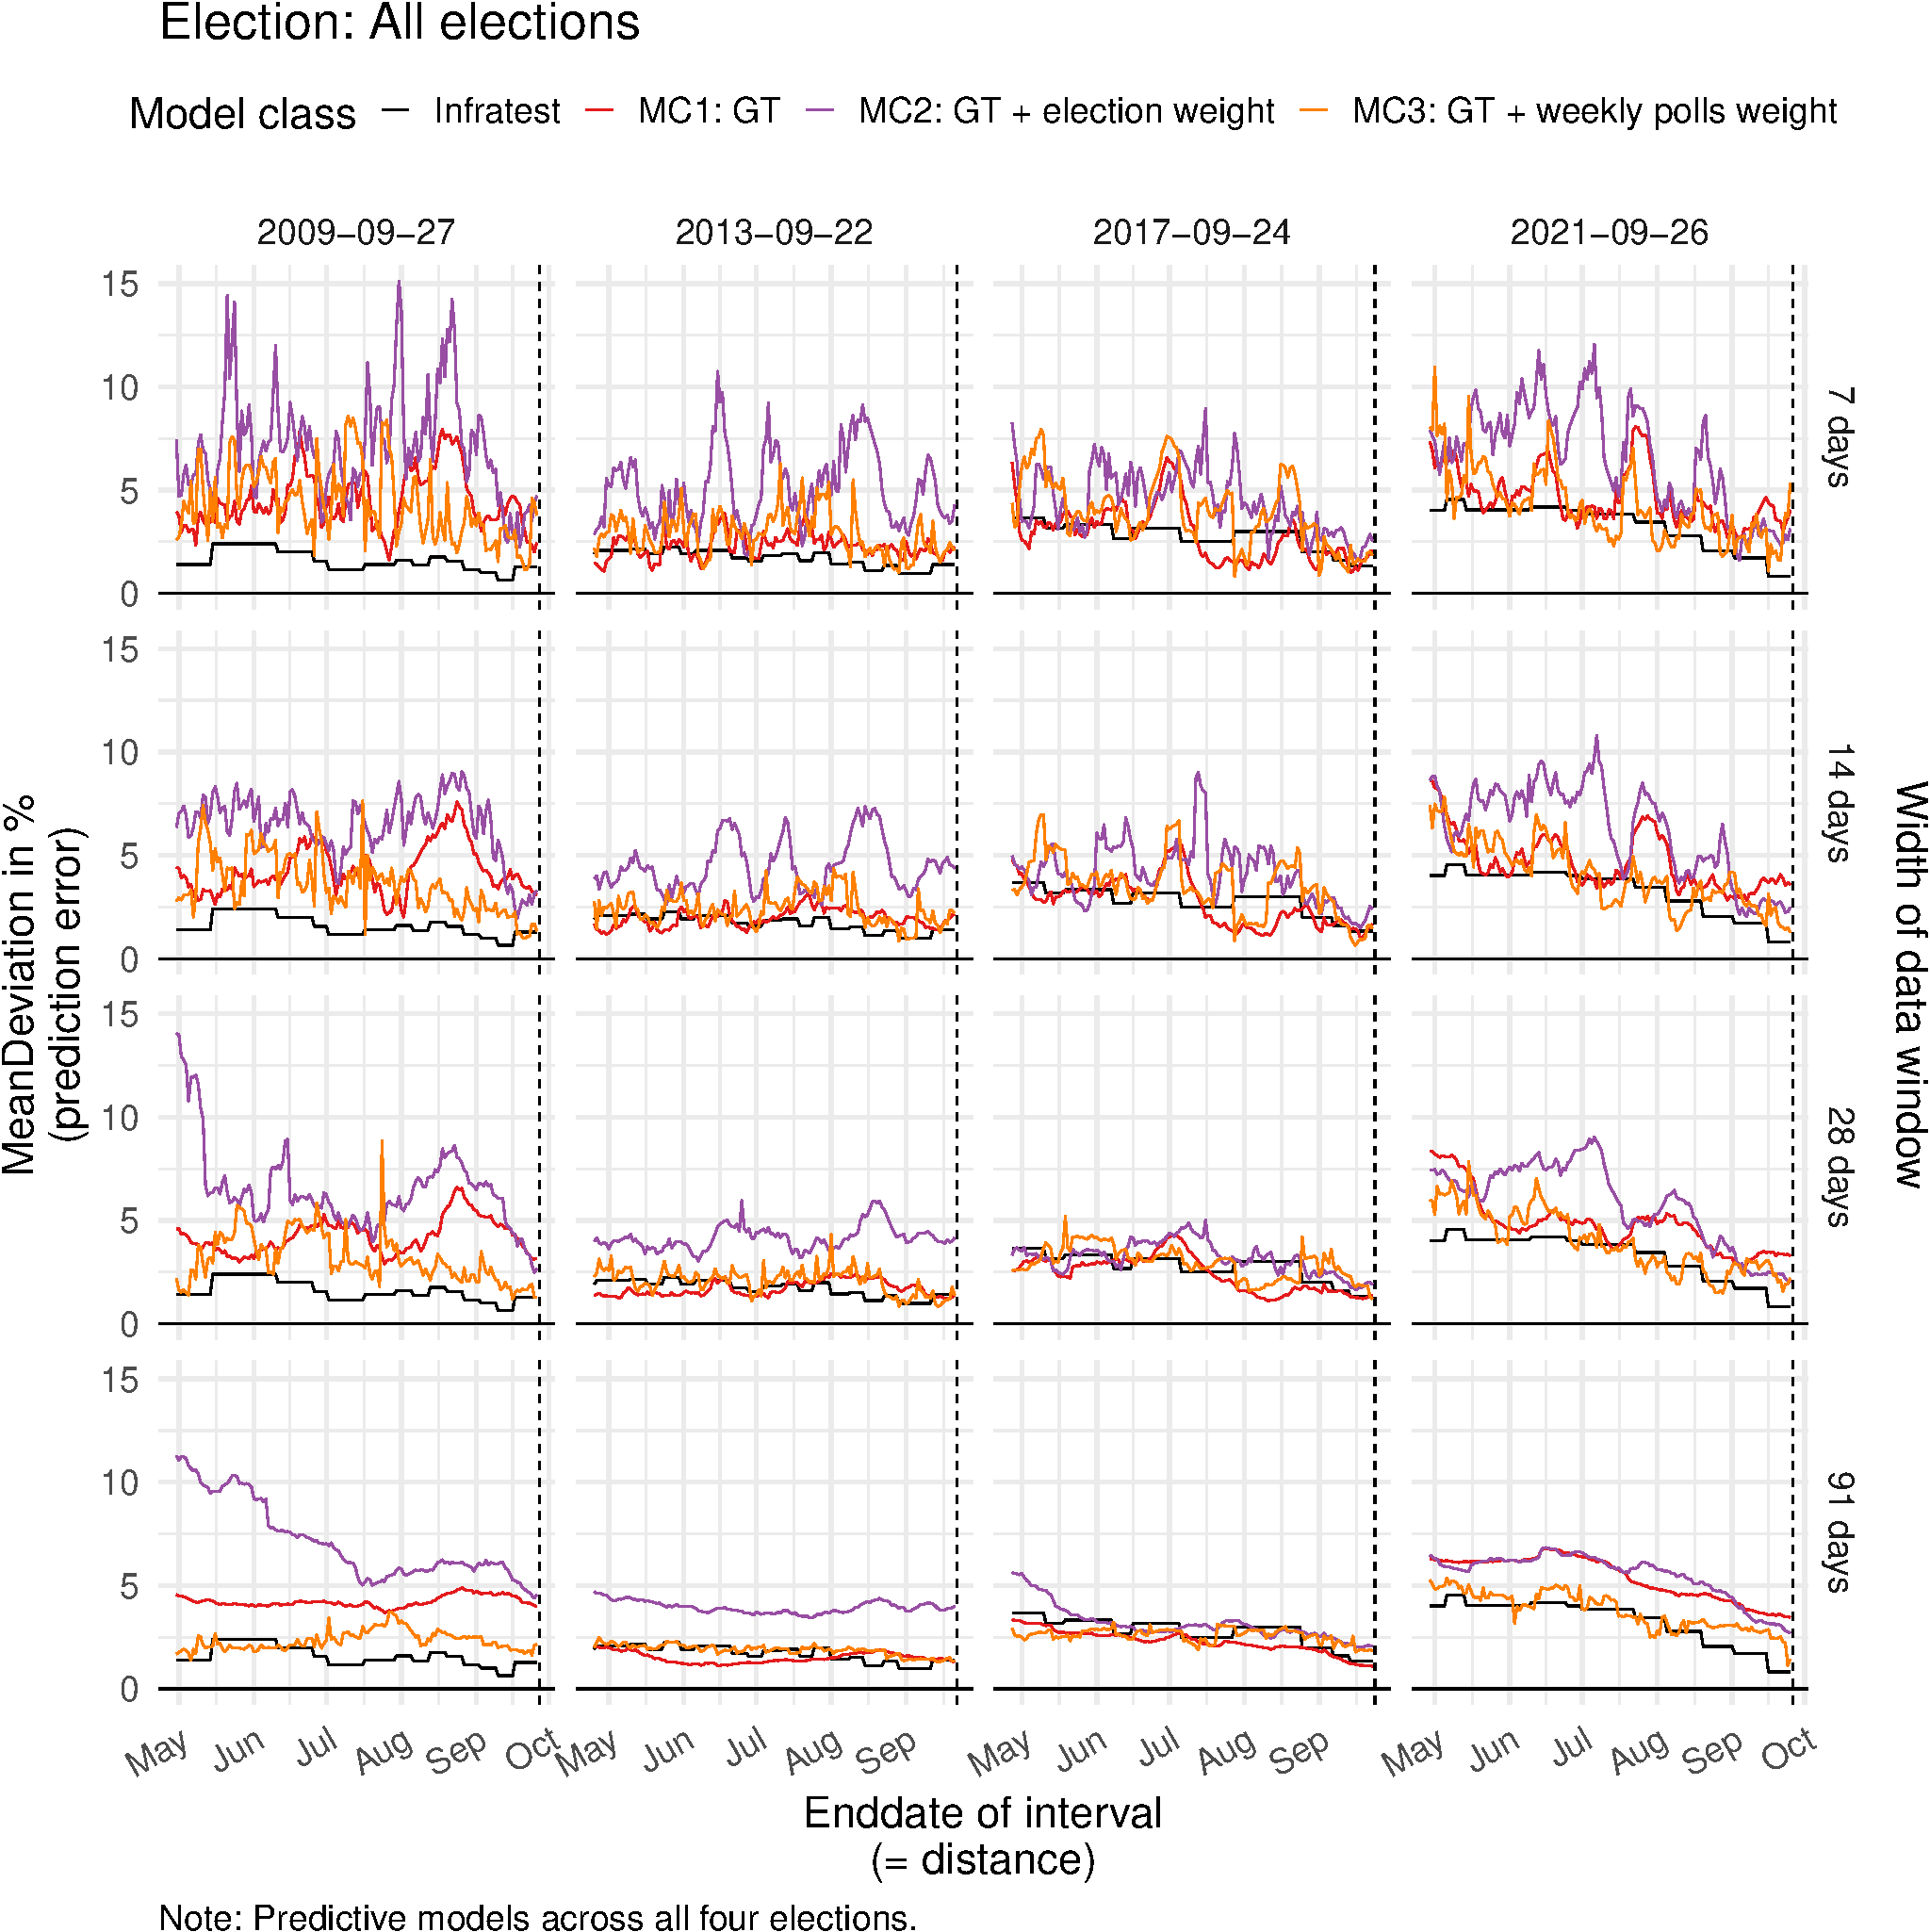
\includegraphics{figures/fig-A9-1.pdf}

}

\end{figure}

\hypertarget{benchmarking-gt-data-and-our-models-against-all-other-leading-polling-institutes}{%
\section{Benchmarking GT data and our models against all other leading
polling
institutes}\label{benchmarking-gt-data-and-our-models-against-all-other-leading-polling-institutes}}

Figure~\ref{fig-A10} and Figure~\ref{fig-A11} provide a comparison of
our models (and Infratest Dimap) to other polling institutes.

\begin{figure}[H]

\caption{\label{fig-A10}Benchmarking against other polls (Elections:
2009, 2013)}

{\centering 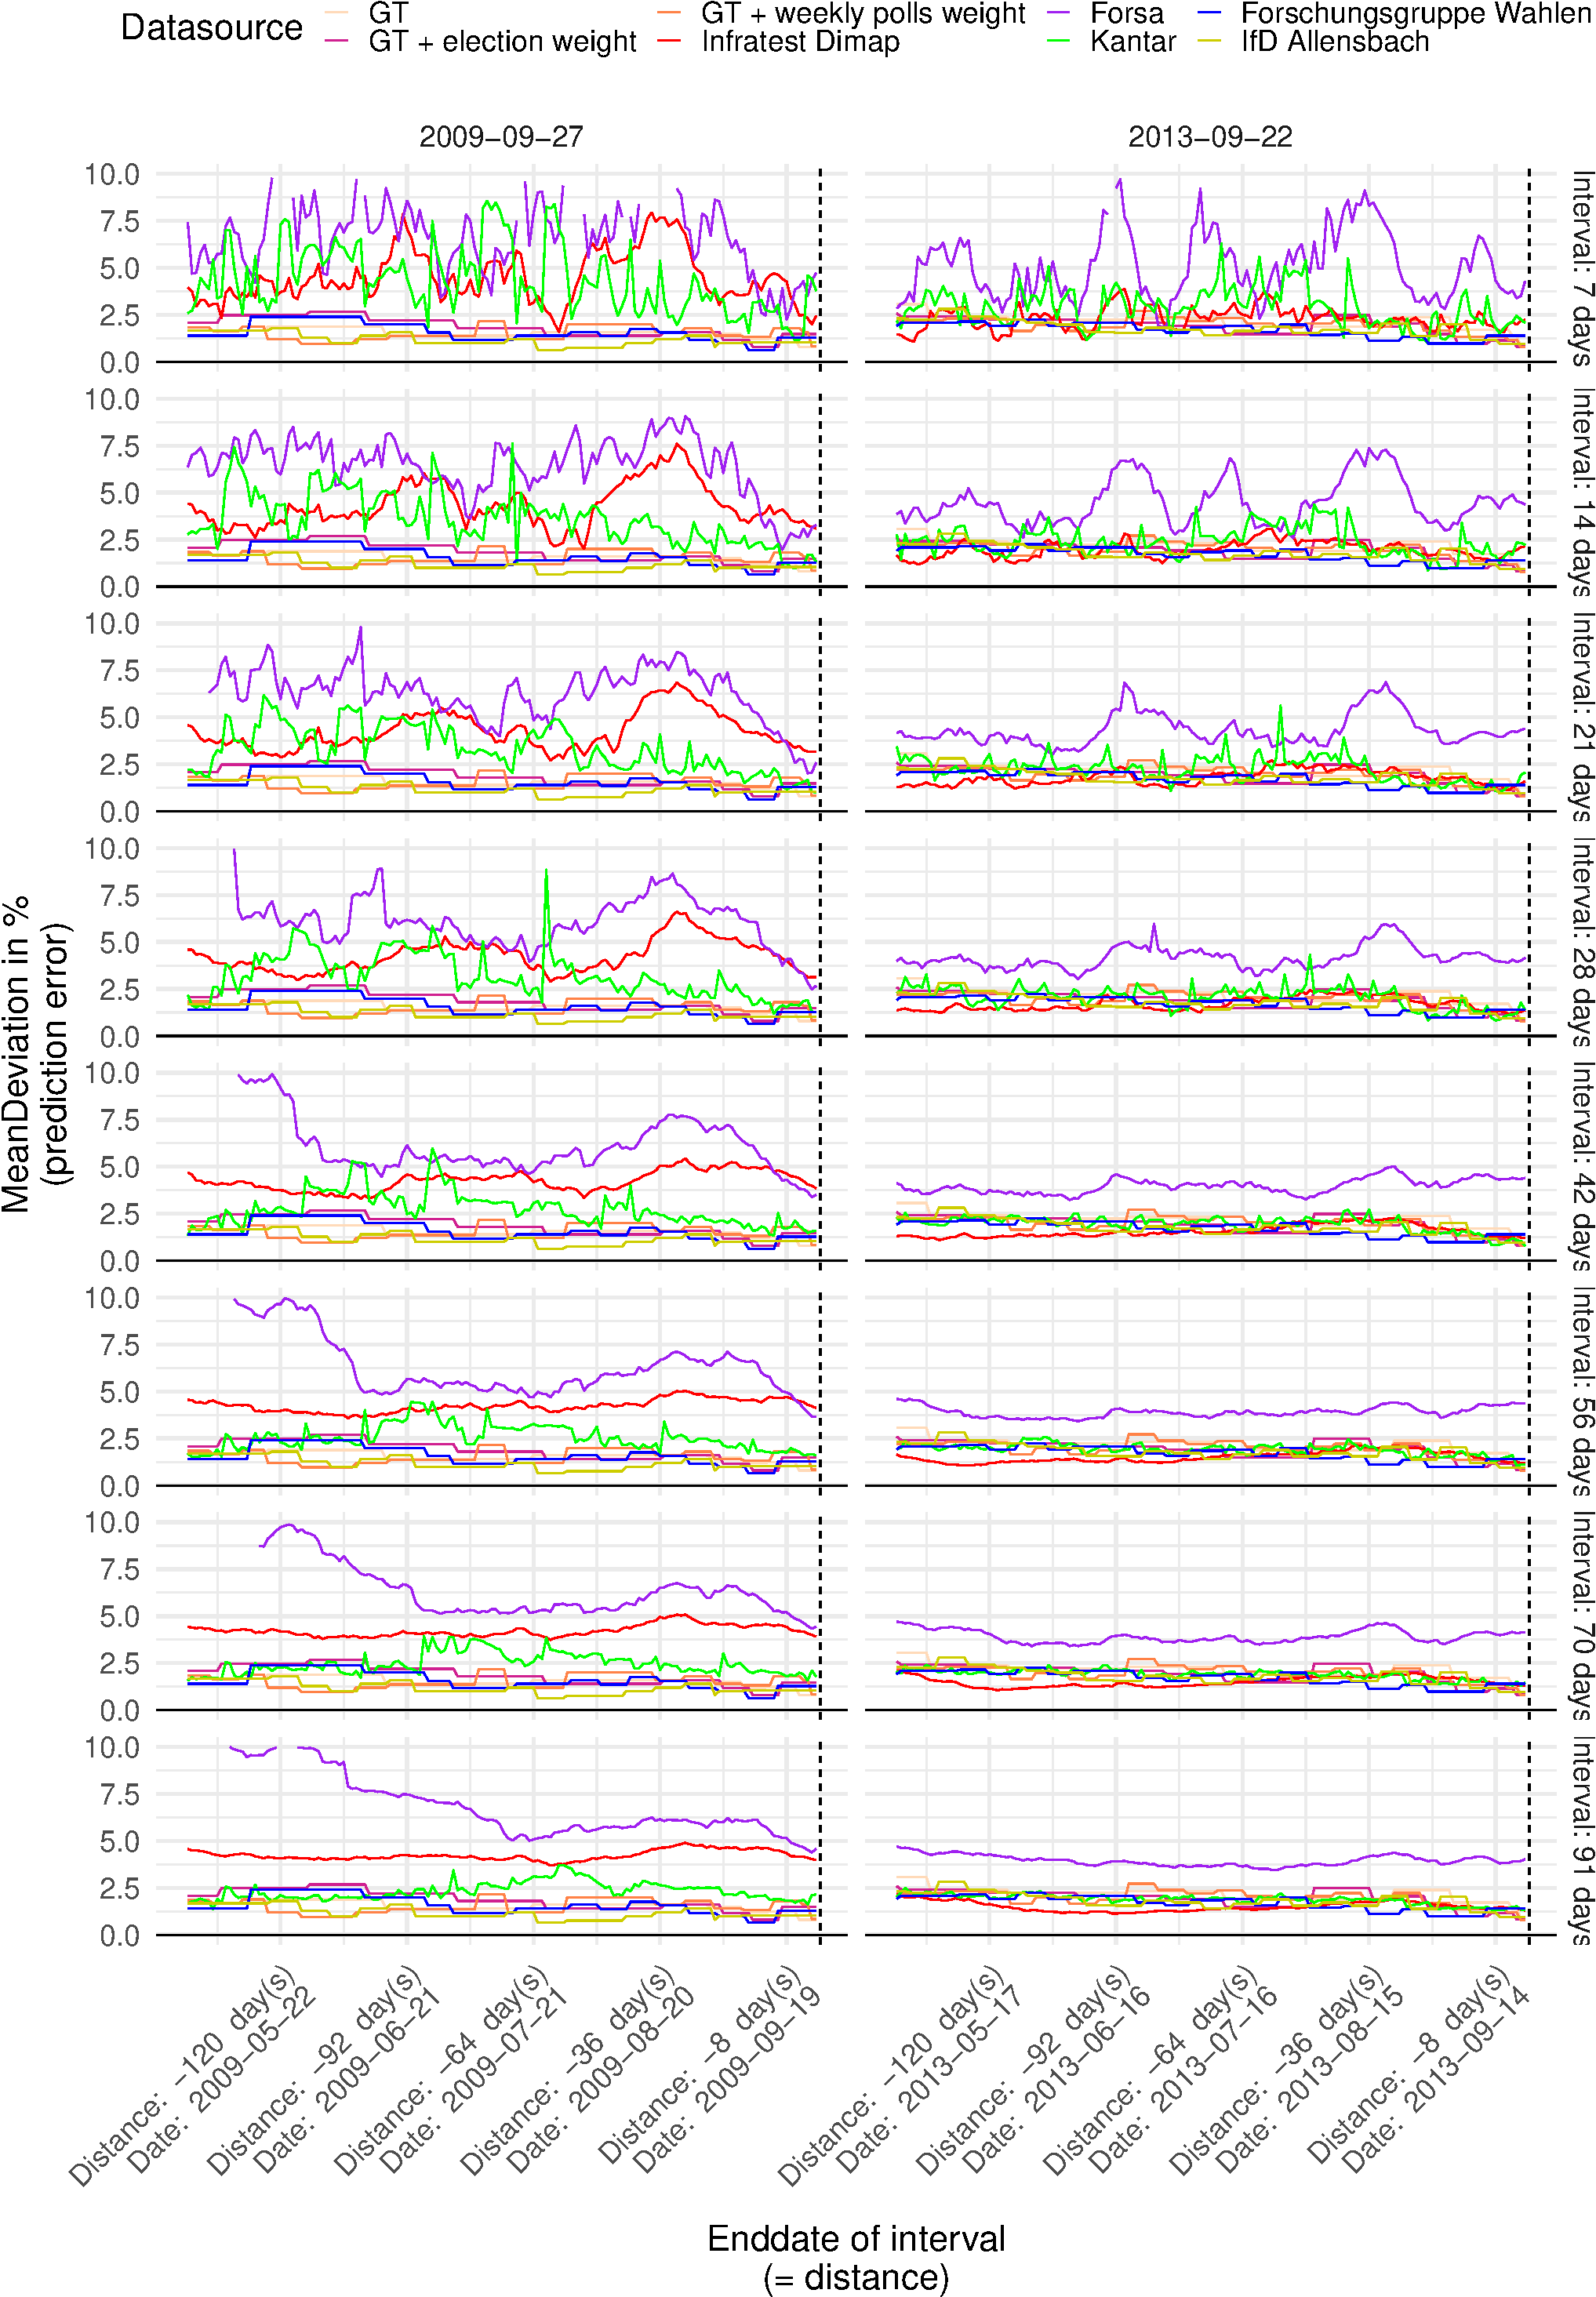
\includegraphics{figures/fig-A10-1.pdf}

}

\end{figure}

\begin{figure}[H]

\caption{\label{fig-A11}Benchmarking against other polls (Elections:
2017, 2021)}

{\centering 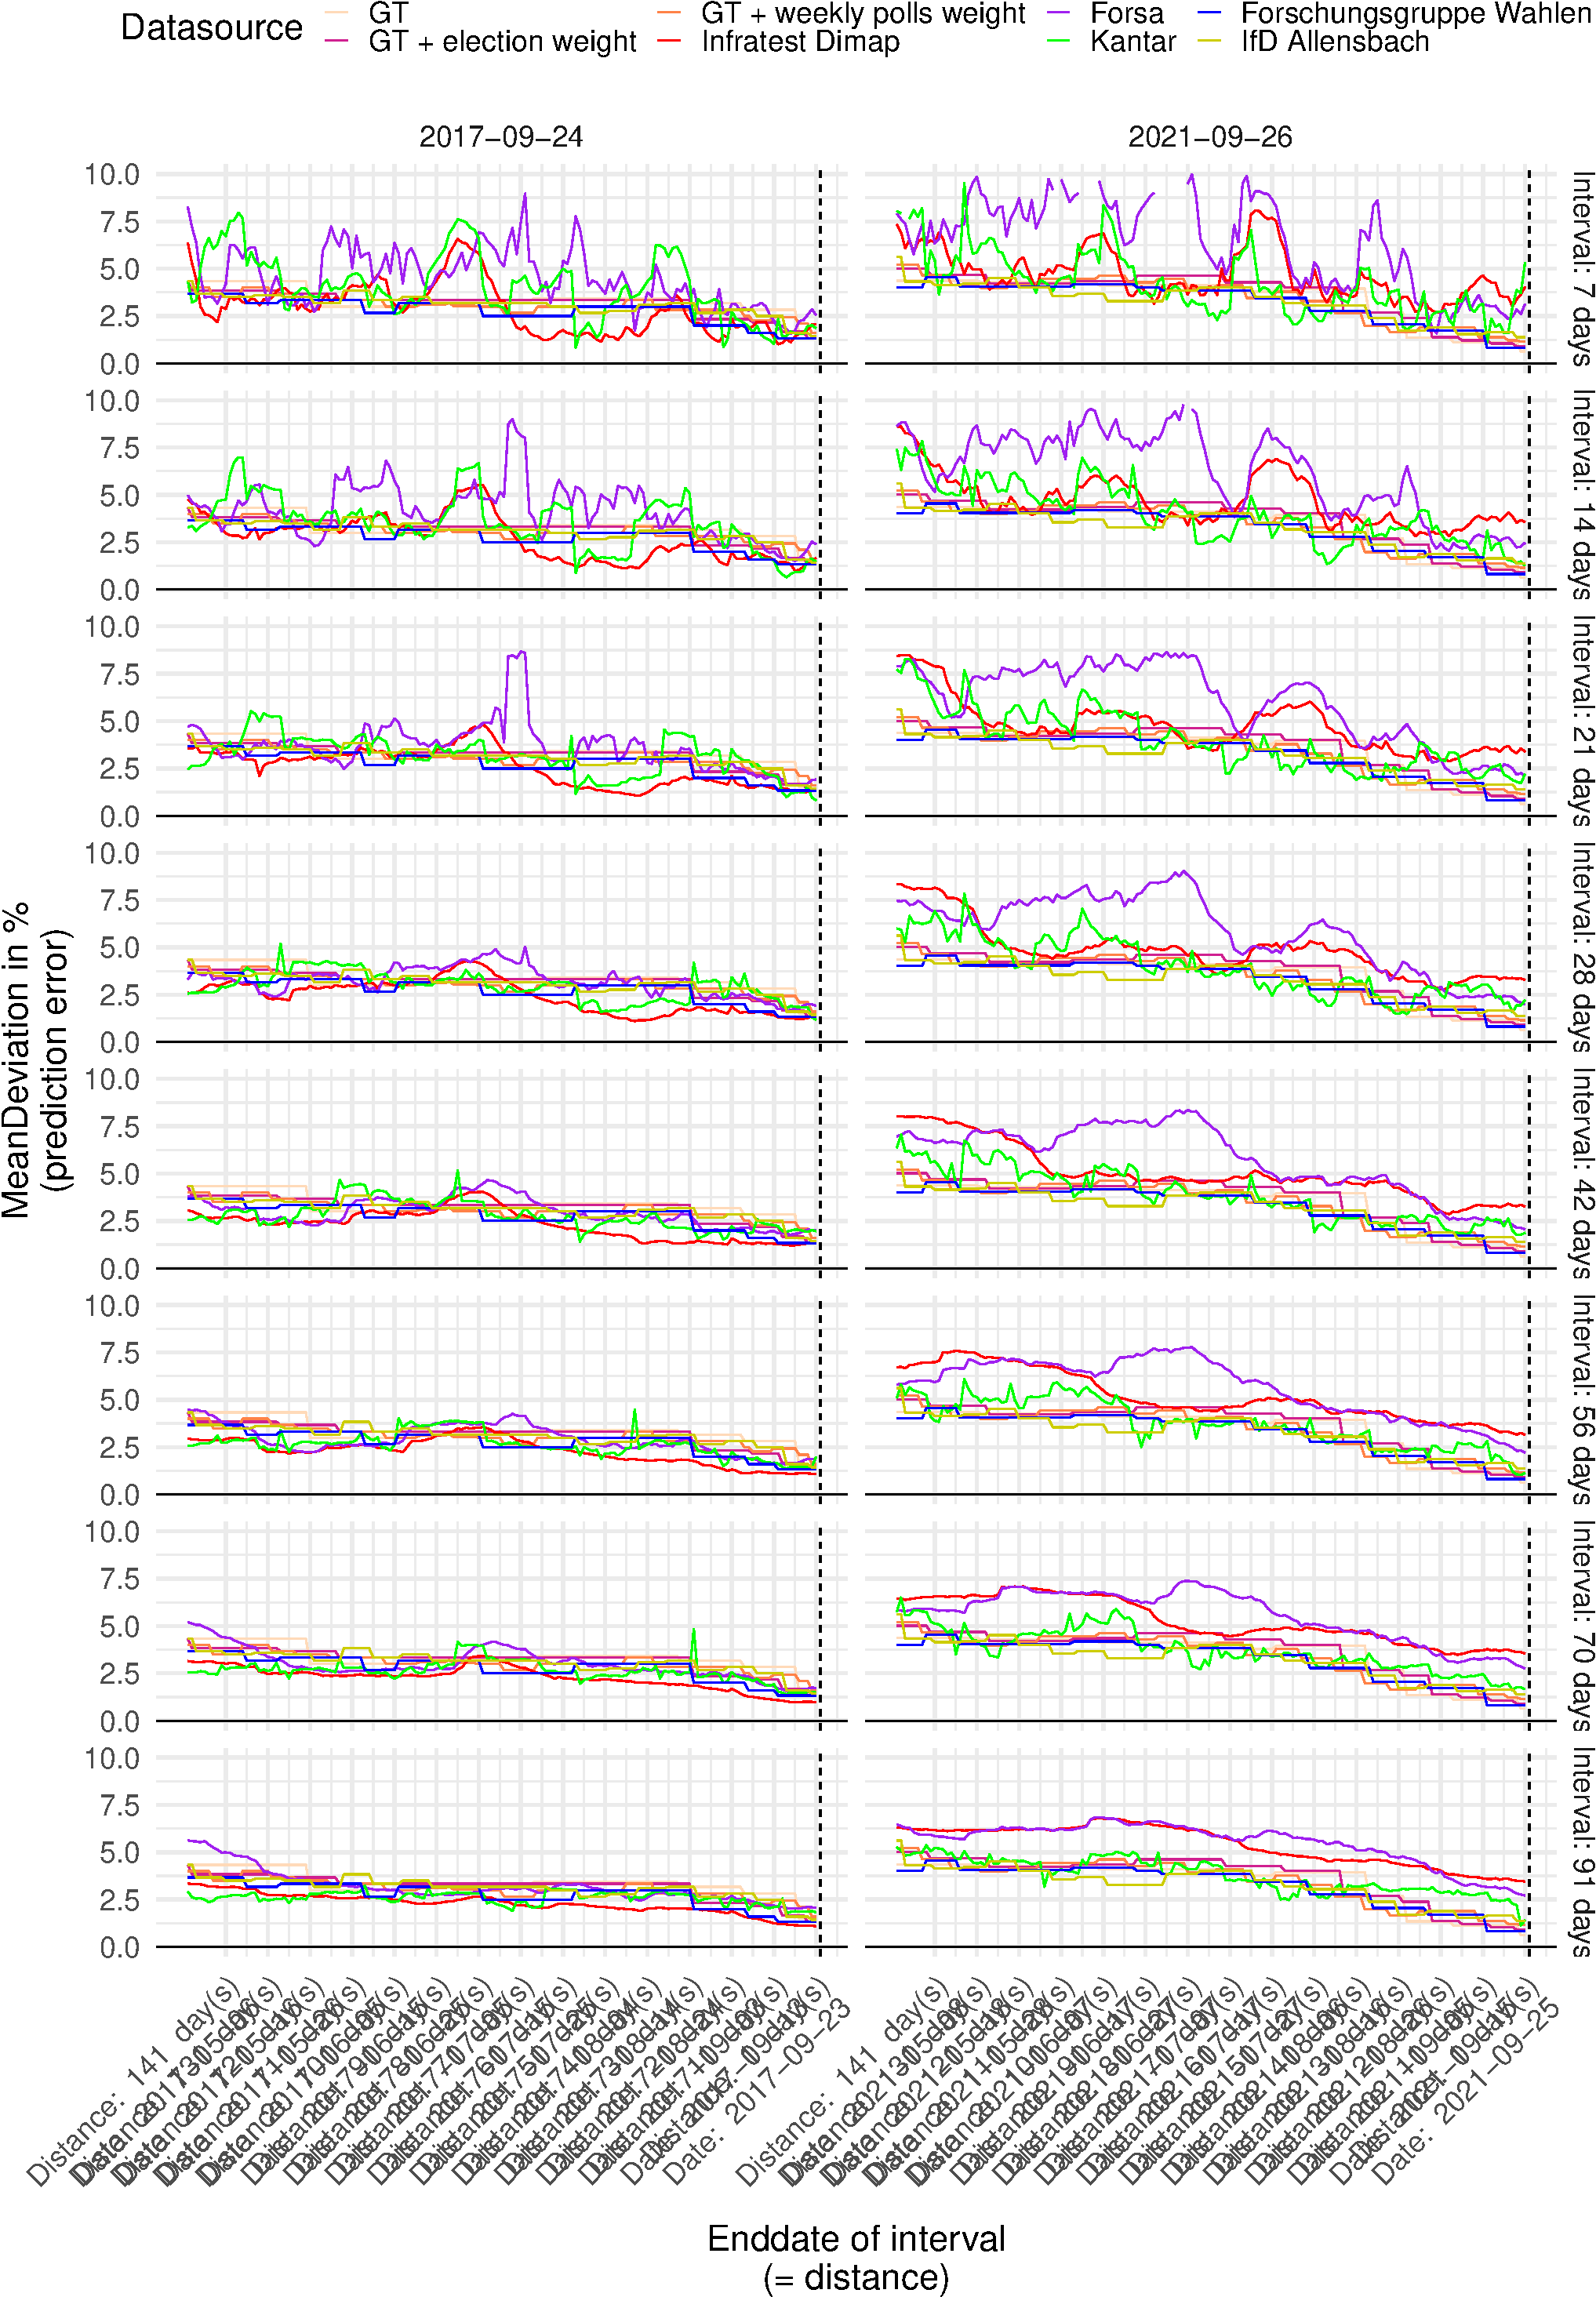
\includegraphics{figures/fig-A11-1.pdf}

}

\end{figure}

\hypertarget{sec-other-parties}{%
\section{Replicating analysis using a ``other parties'' category for GT
data}\label{sec-other-parties}}

fig-A12 to fig-A17 replicate our analysis but this time including a
``other parties'' category for GT data. The corresponding results reveal
patterns similar to the ones discussed in the main paper.

\begin{figure}[H]

\caption{\label{fig-A12}Figure 4 with `other parties'}

{\centering 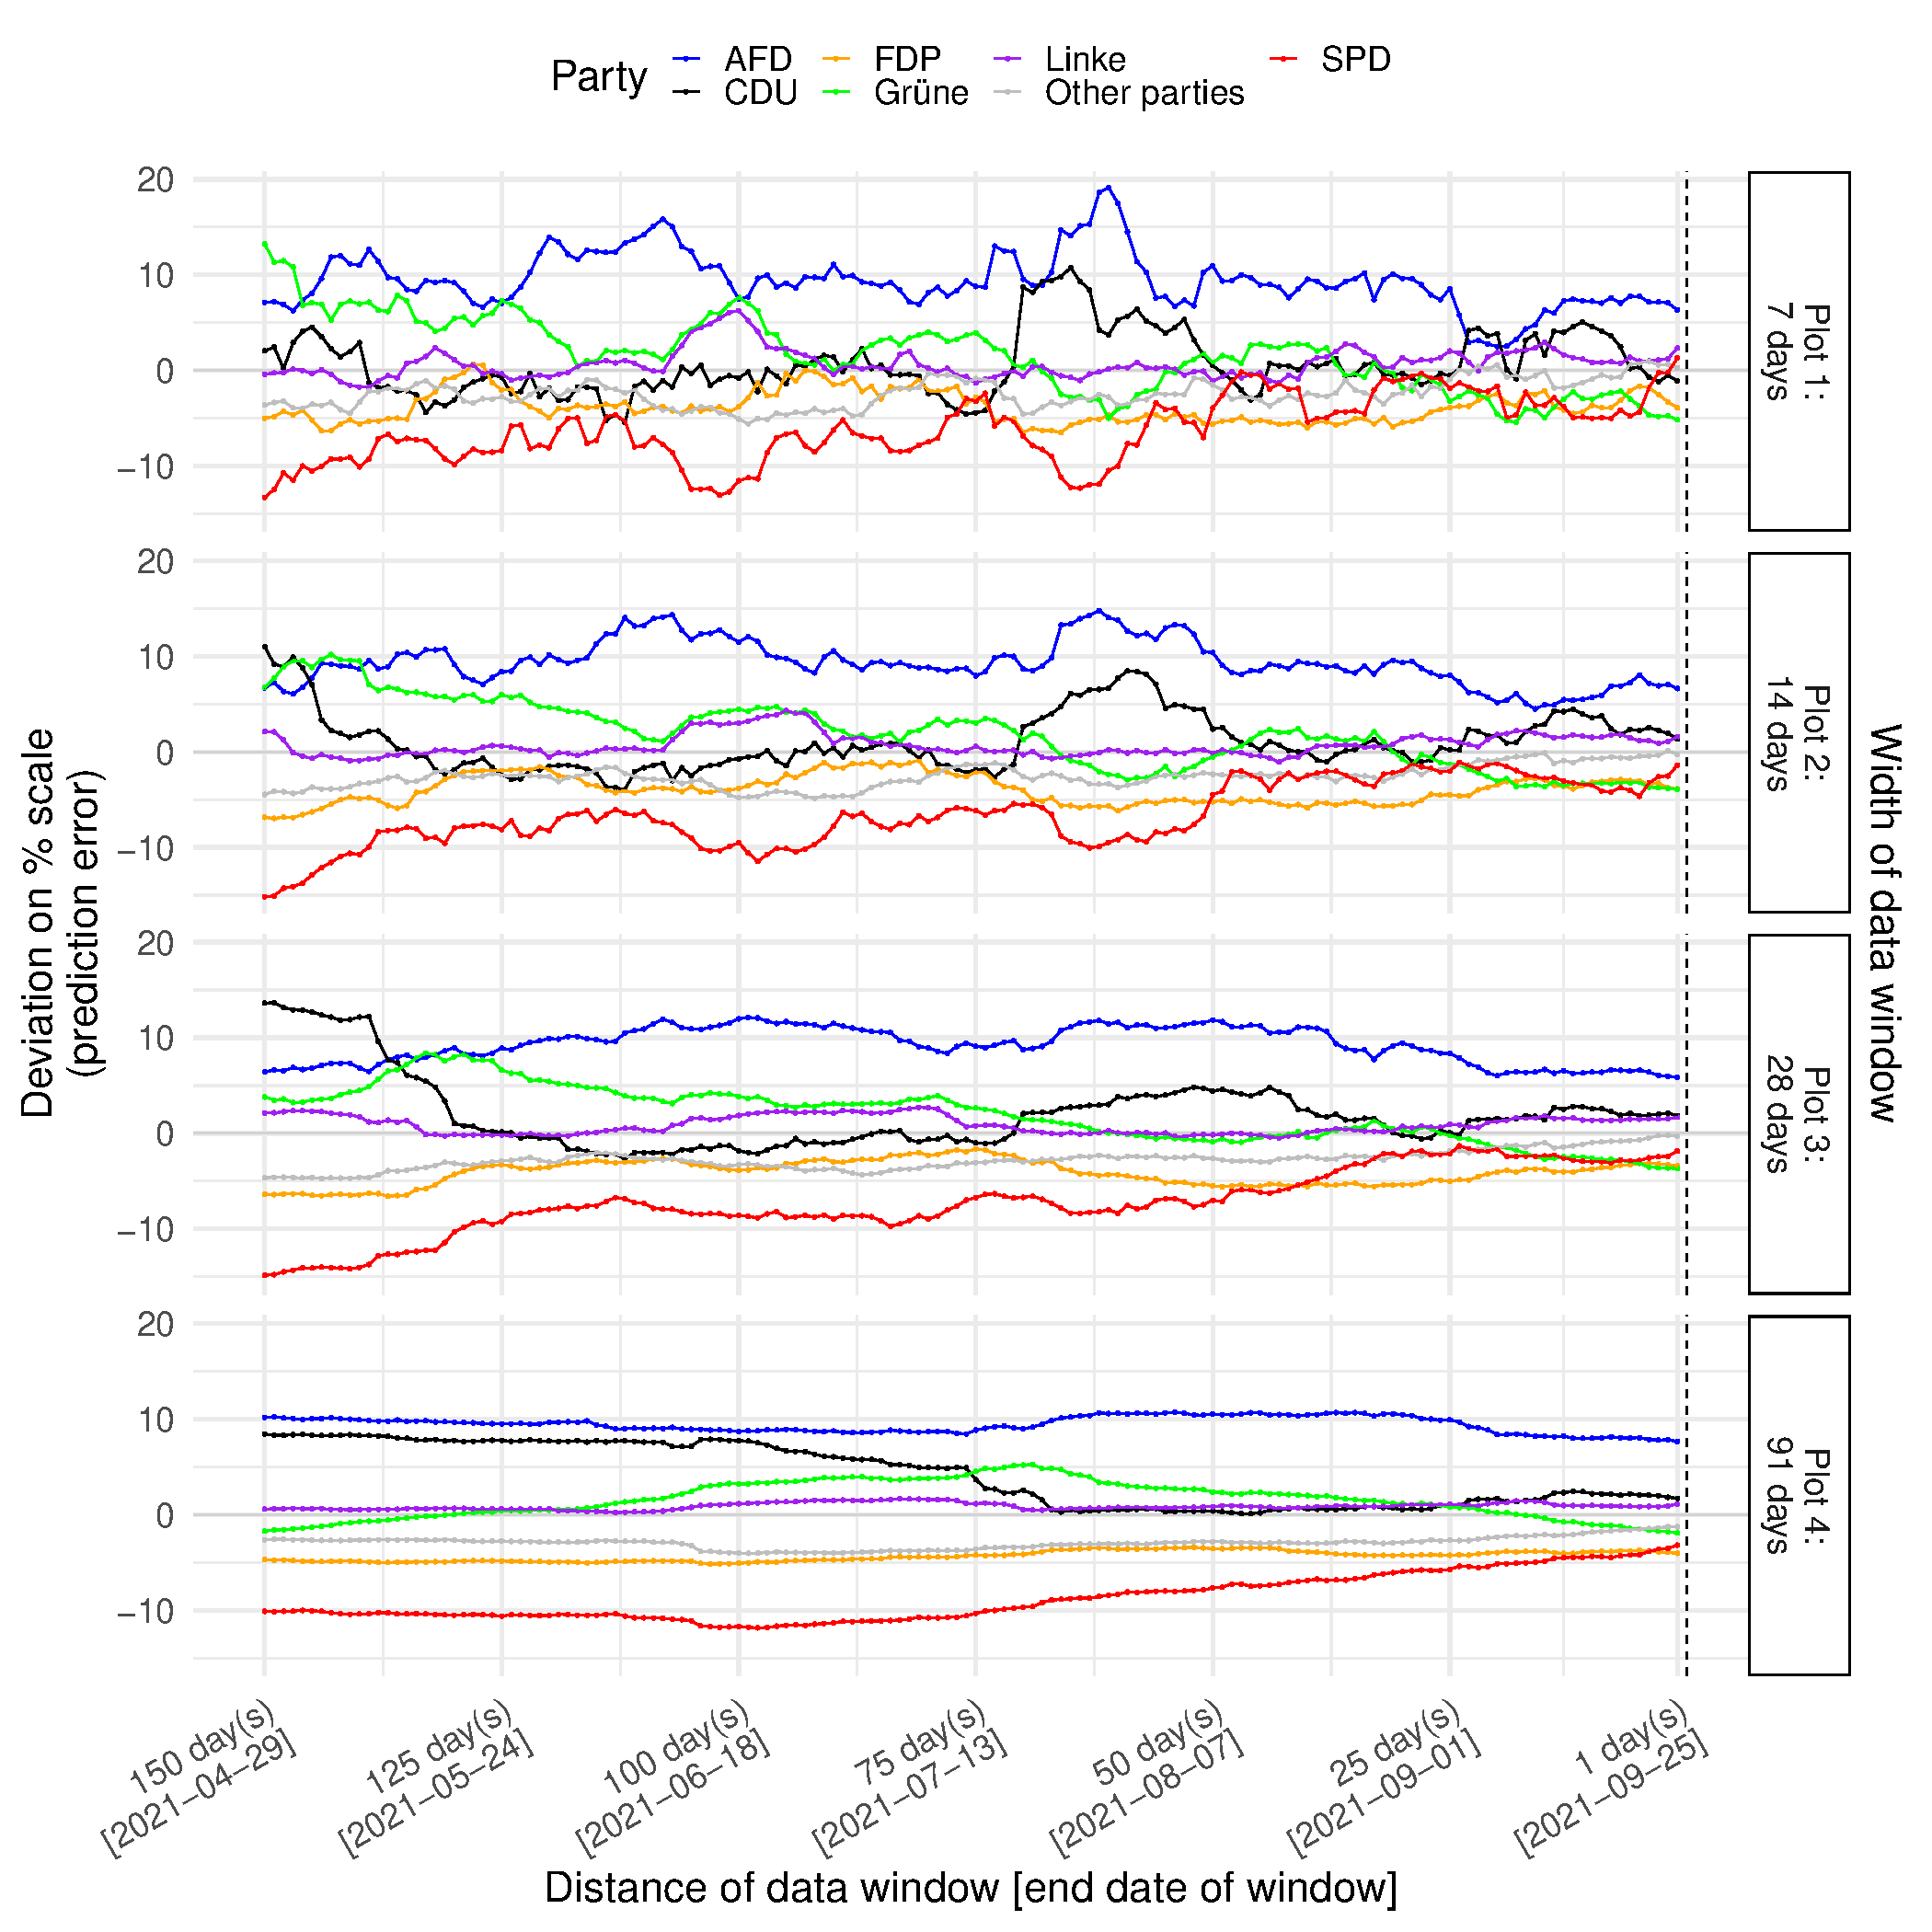
\includegraphics{figures/fig-A12-1.pdf}

}

\end{figure}

\begin{figure}[H]

\caption{\label{fig-A13}Figure 5 with `other parties' (2021 election)}

{\centering 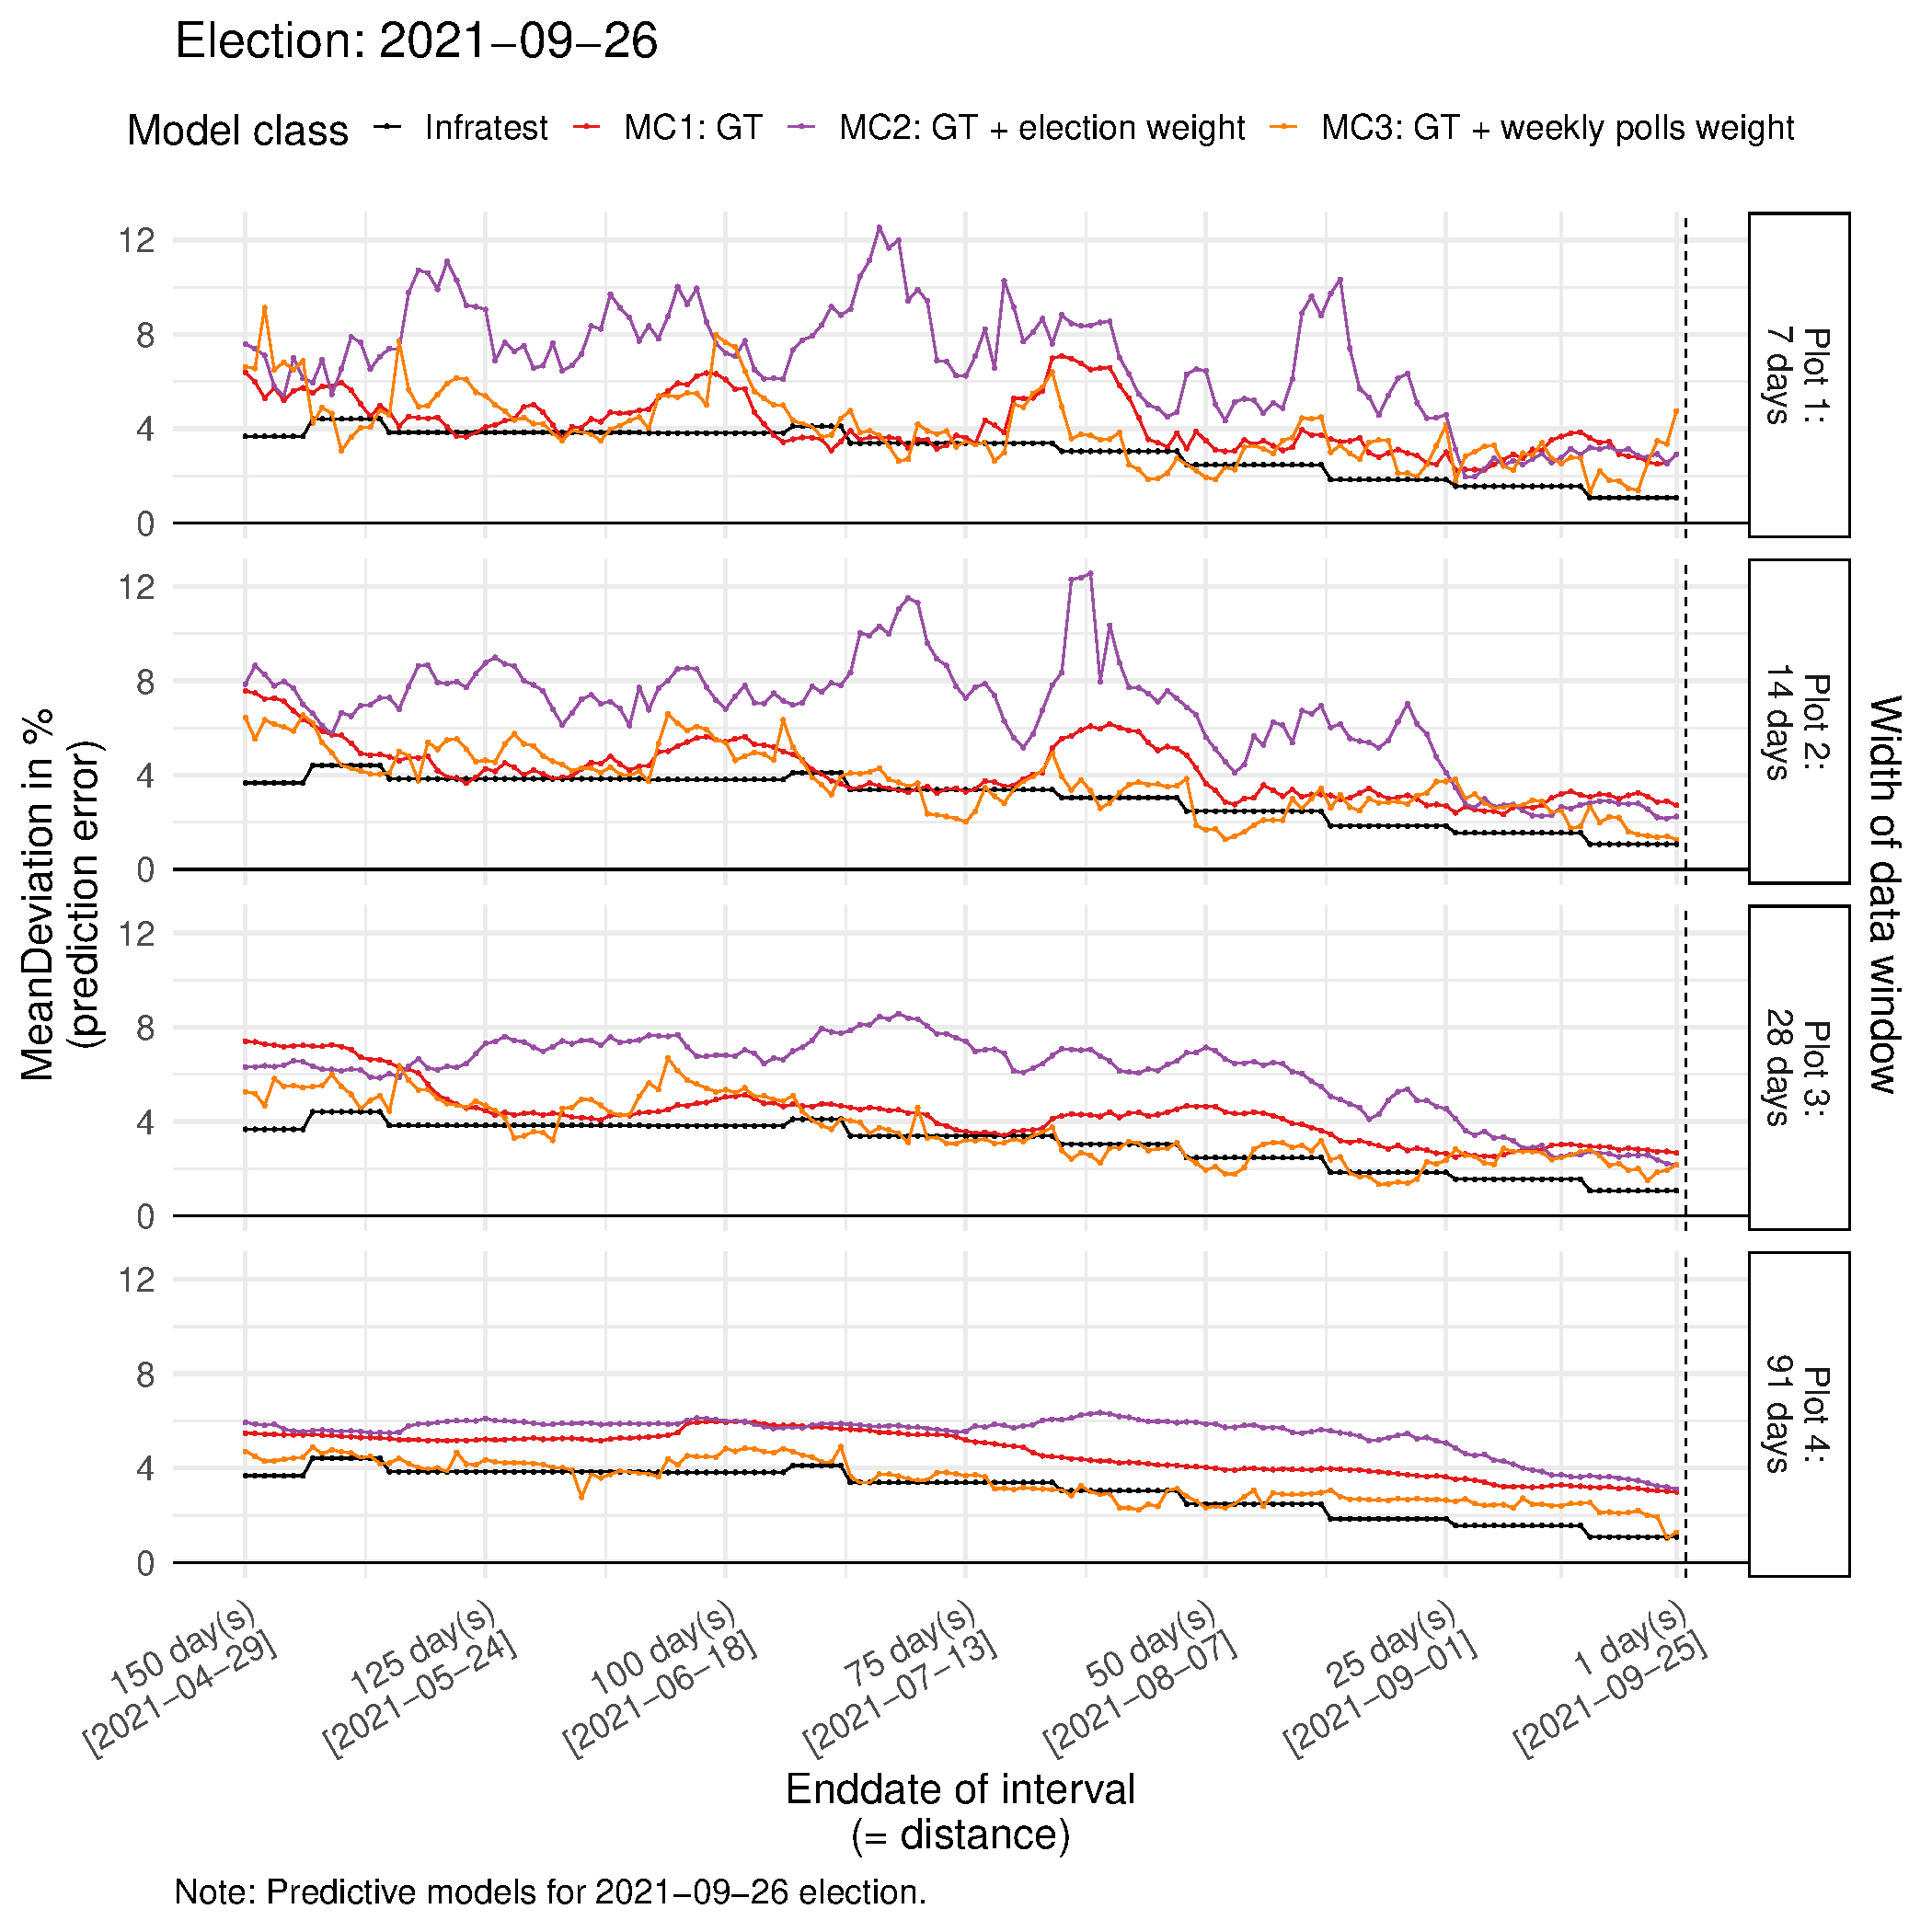
\includegraphics{figures/fig-A13-1.pdf}

}

\end{figure}

\begin{figure}[H]

\caption{\label{fig-A14}Figure 5 with `other parties' (2009 election)}

{\centering 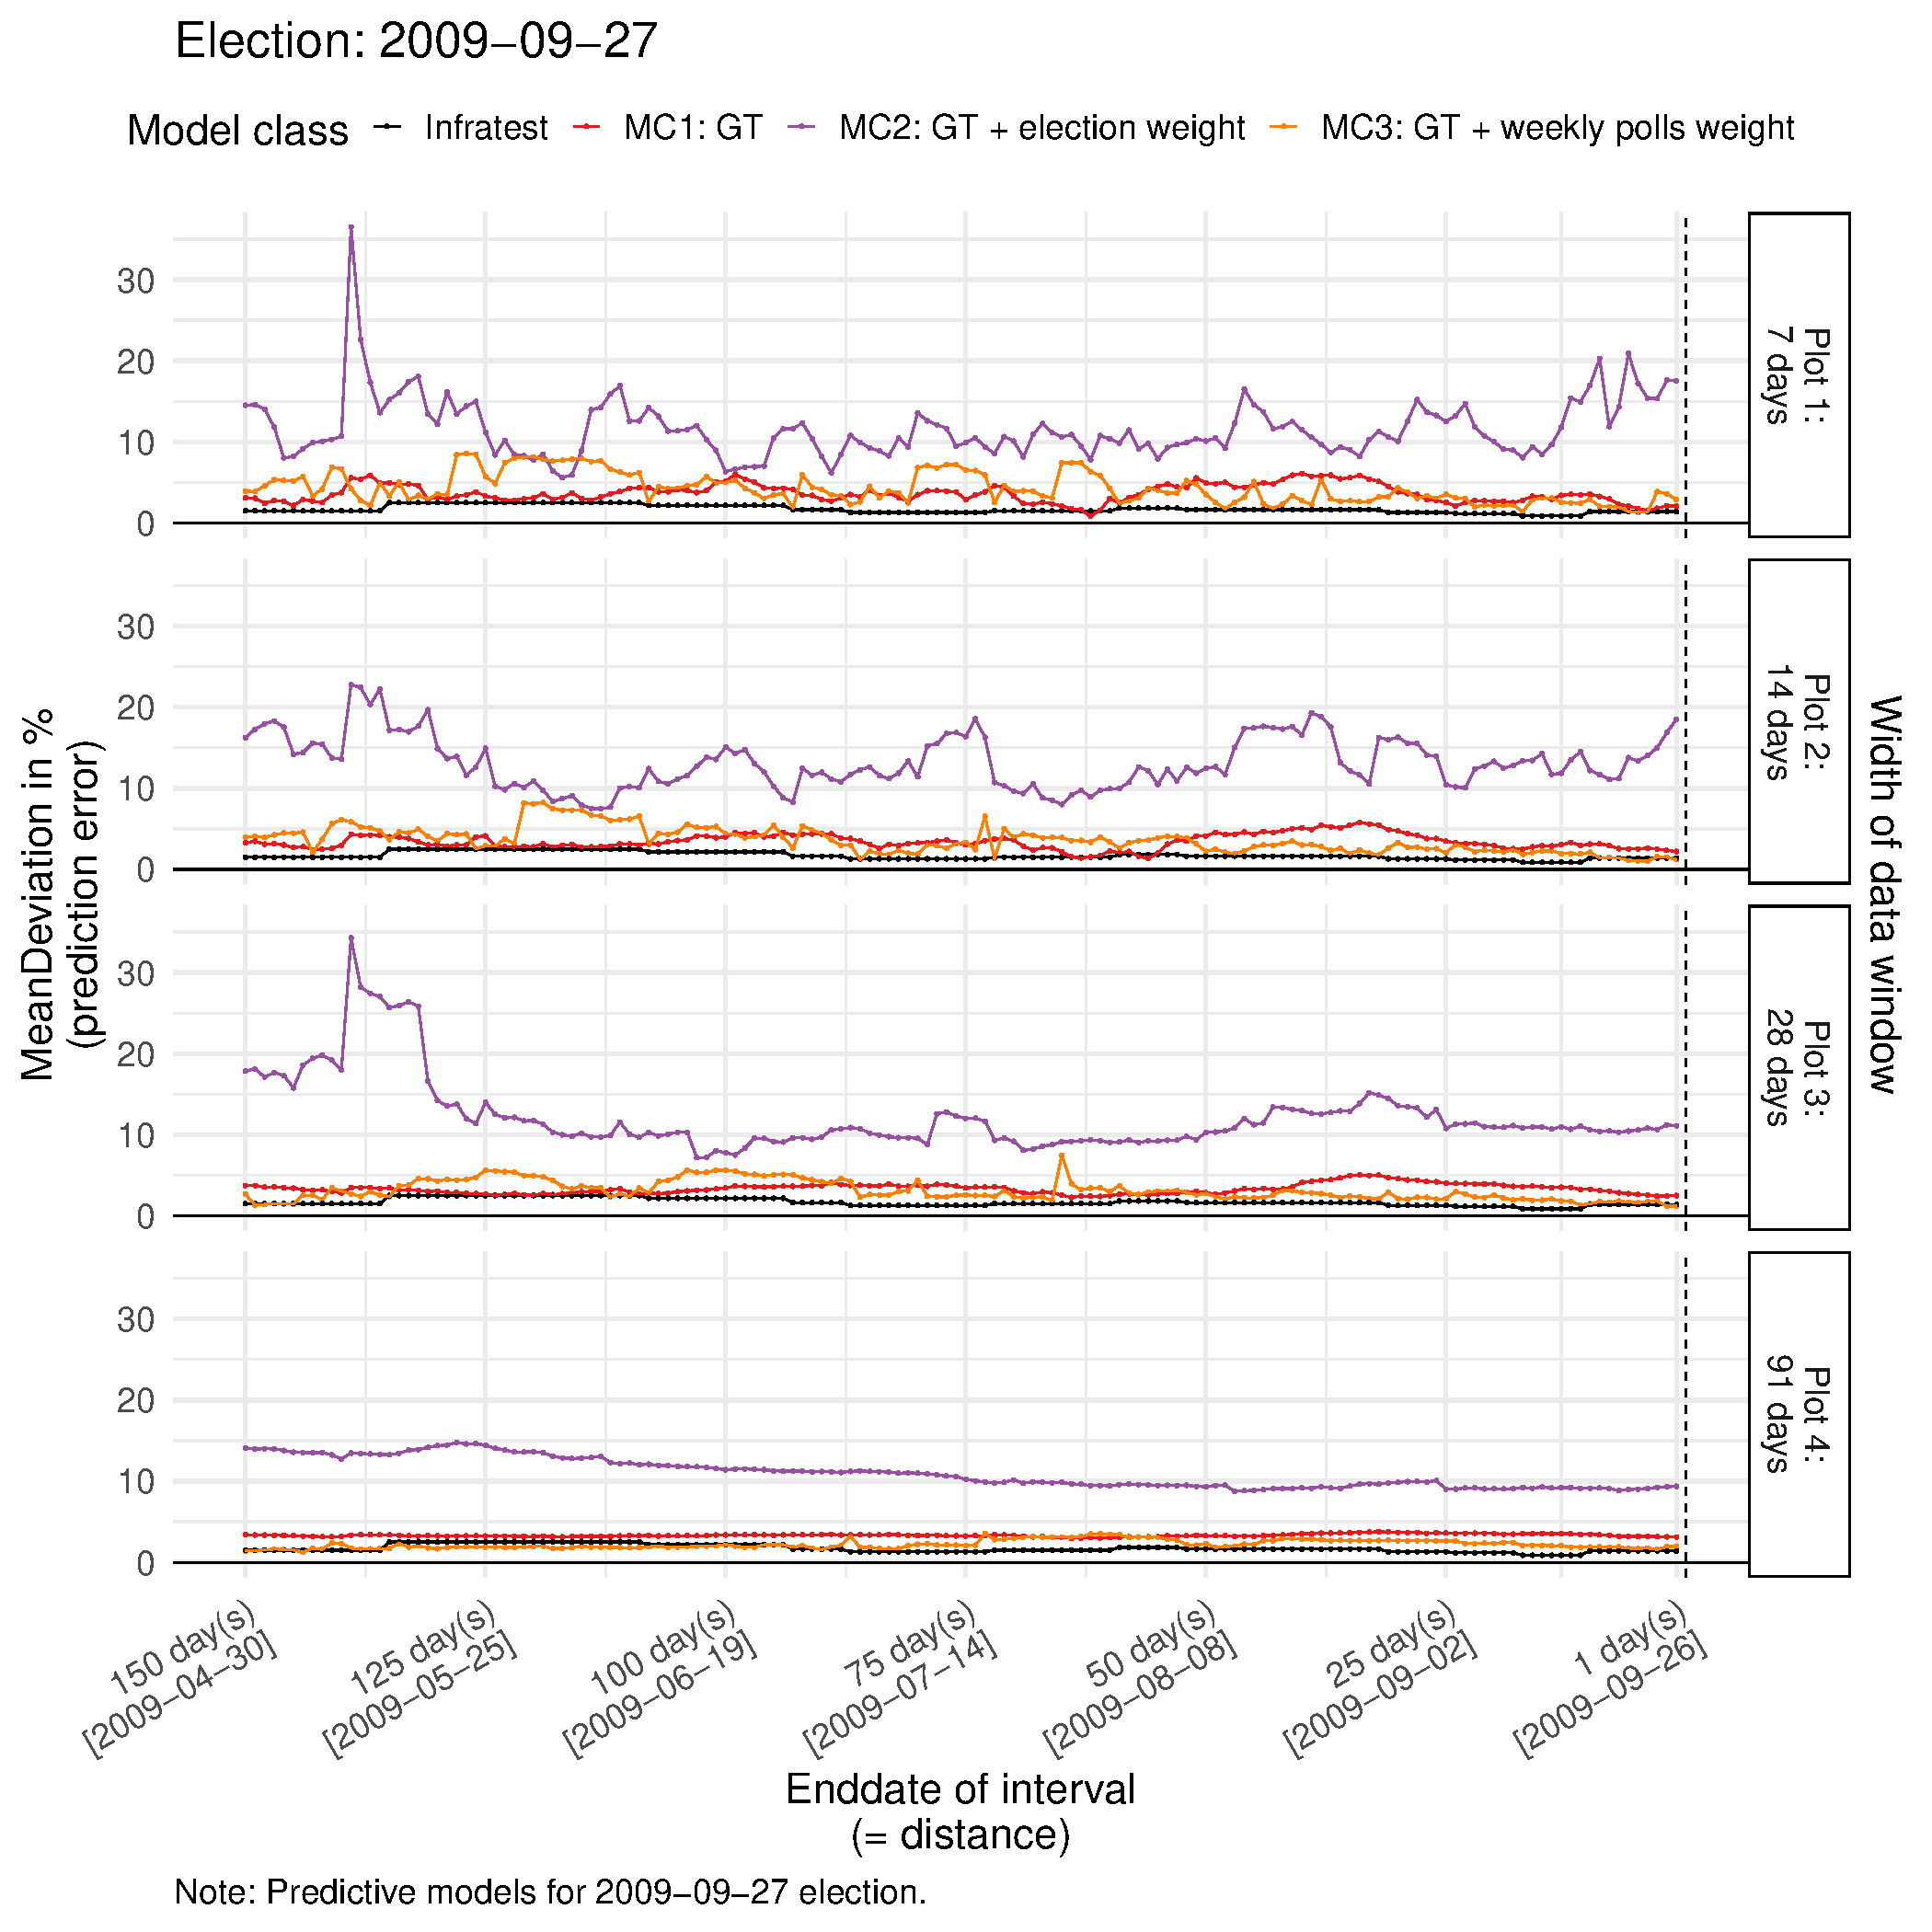
\includegraphics{figures/fig-A14-1.pdf}

}

\end{figure}

\begin{figure}[H]

\caption{\label{fig-A15}Figure 5 with `other parties' (2013 election)}

{\centering 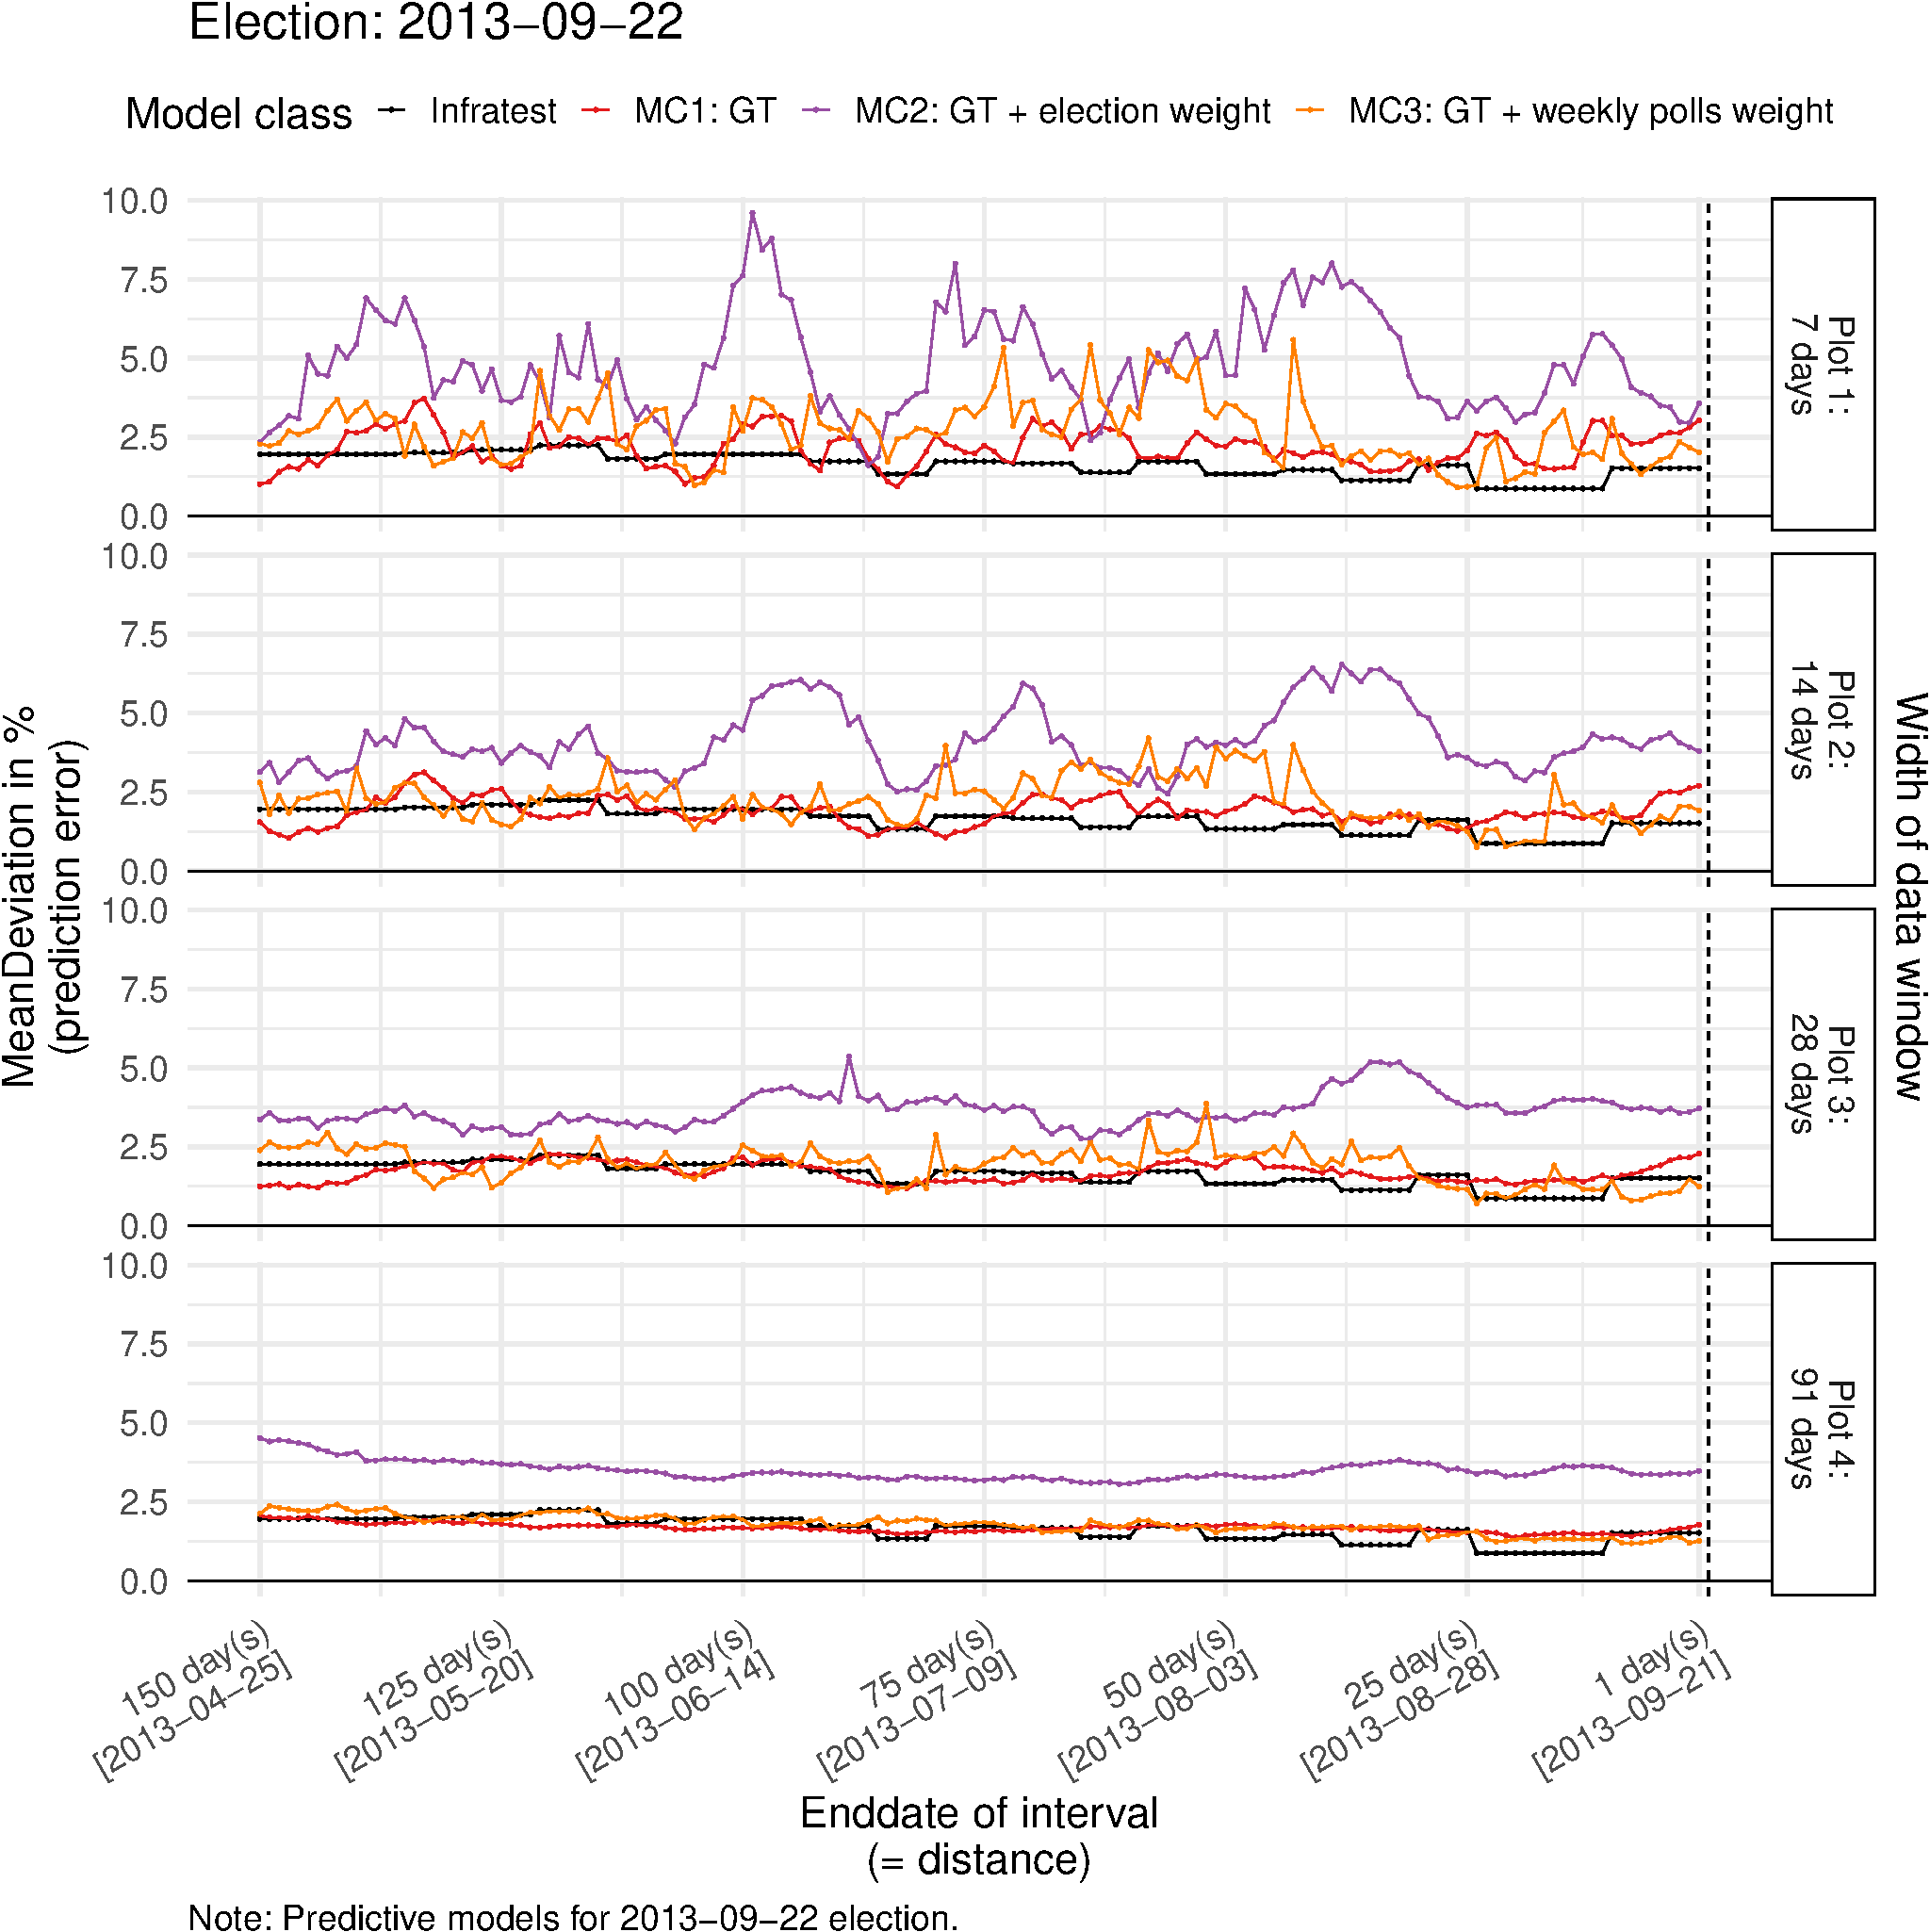
\includegraphics{figures/fig-A15-1.pdf}

}

\end{figure}

\begin{figure}[H]

\caption{\label{fig-A16}Figure 5 with `other parties' (2017 election)}

{\centering 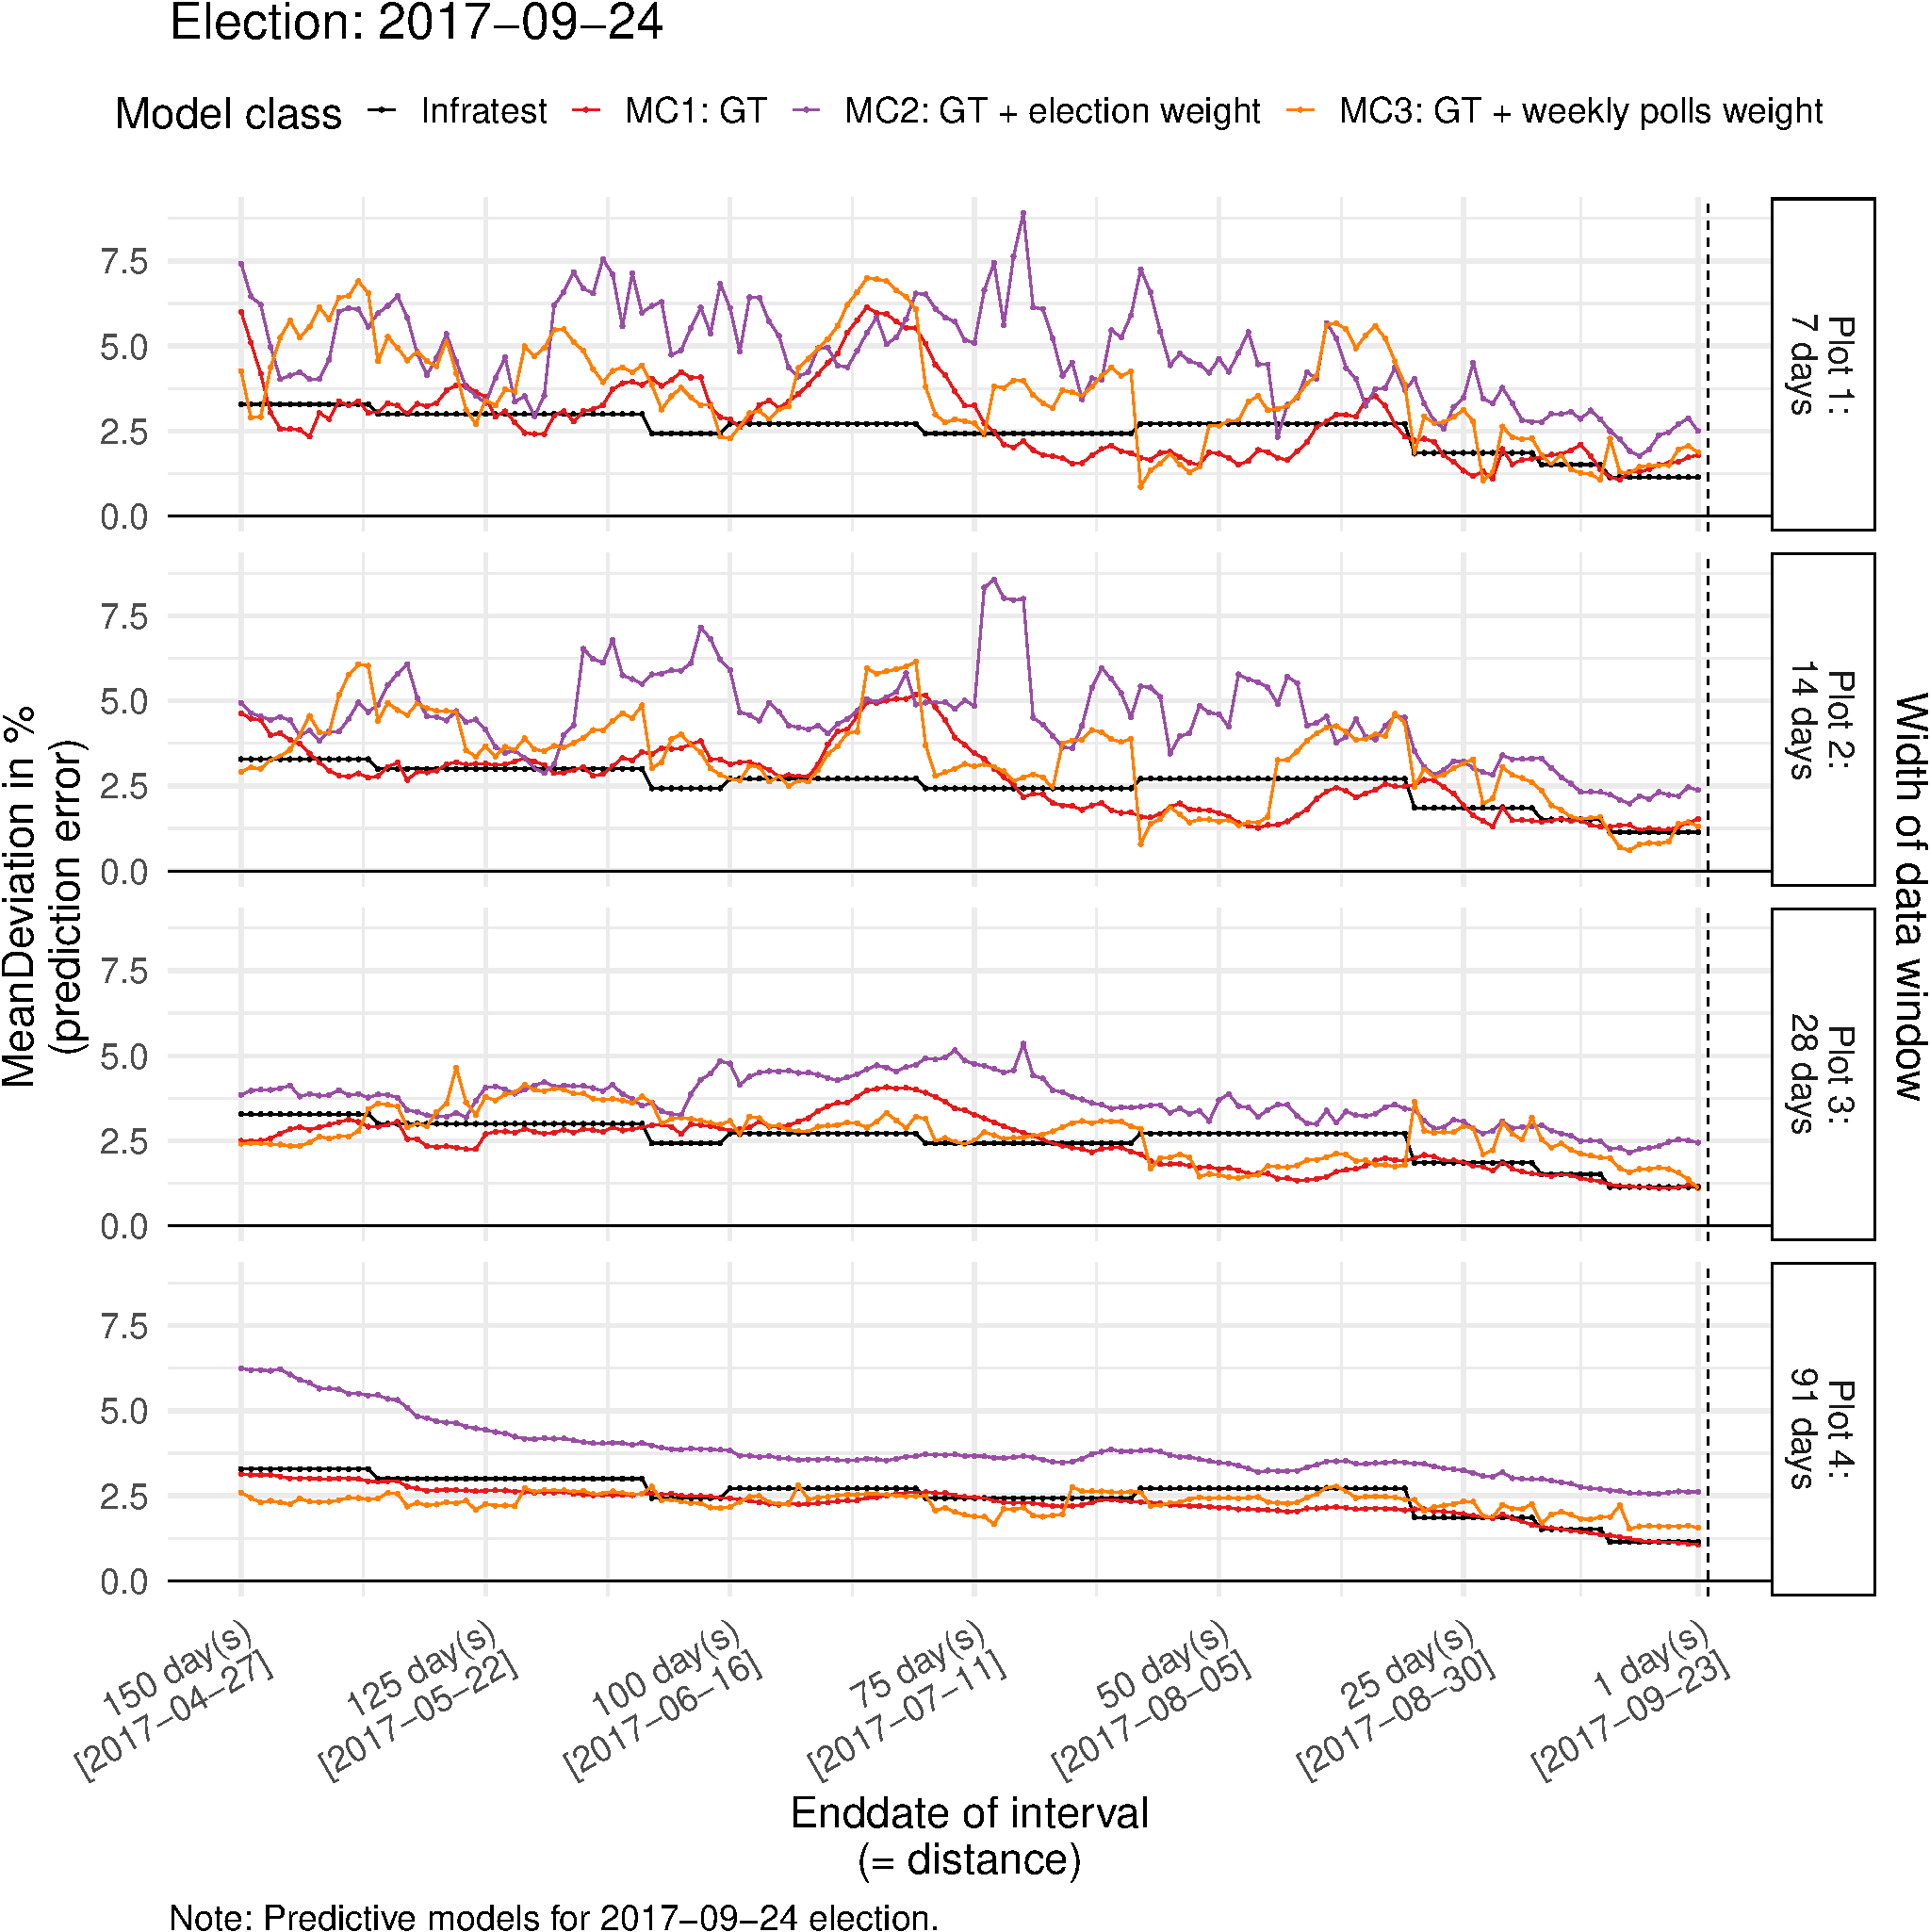
\includegraphics{figures/fig-A16-1.pdf}

}

\end{figure}

\begin{figure}[H]

\caption{\label{fig-A17}Figure 6 with `other parties'}

{\centering 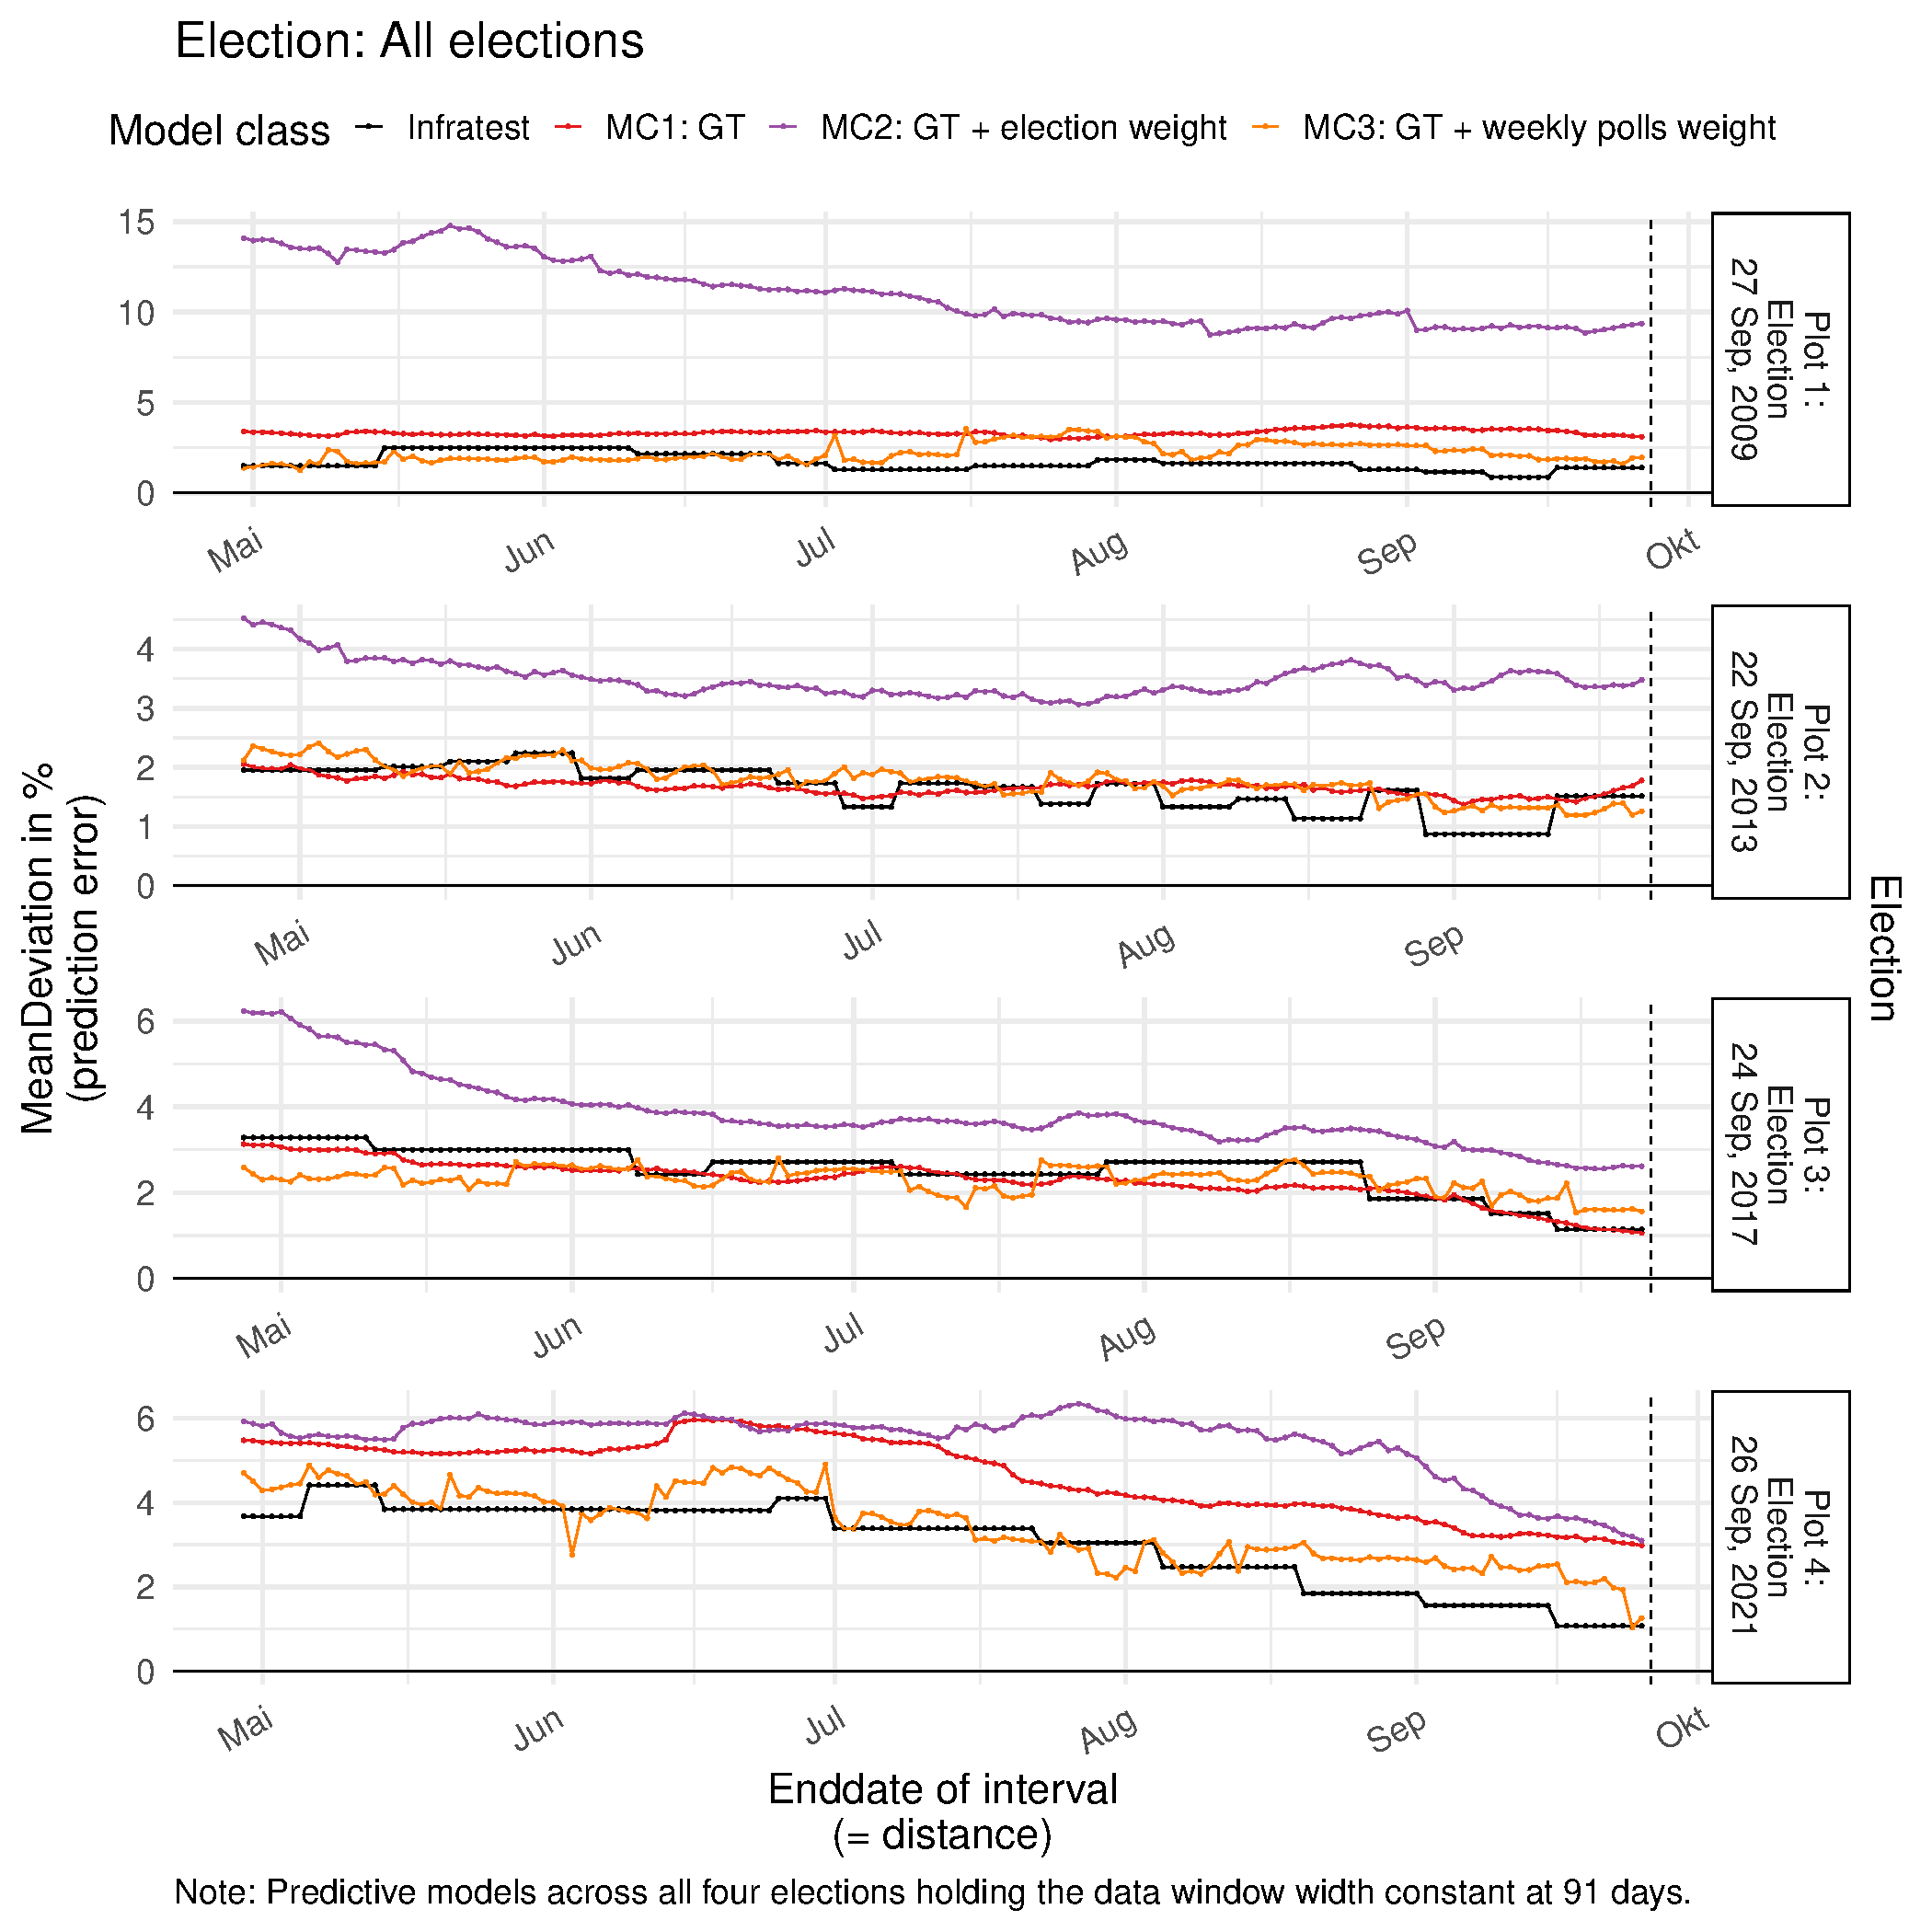
\includegraphics{figures/fig-A17-1.pdf}

}

\end{figure}

\hypertarget{reproducing-and-replicating-this-study}{%
\section{Reproducing and replicating this
study}\label{reproducing-and-replicating-this-study}}

One of our objectives with this study was to provide other researchers
with a transparent workflow that involves all the steps from collecting
the raw GT data, obtaining the predictions, to producing the analyses
and the study itself. The replication files contain the following code
files that correspond to the steps we followed to conduct this study:

\begin{itemize}
\tightlist
\item
  Step 1: Collect polling data
  (\texttt{1\_Step\_1\_collect\_polling\_data.R})

  \begin{itemize}
  \tightlist
  \item
    Contains the code to collect polling data from different polling
    companies in Germany including Infratest Dimap.
  \item
    Creates files ``data\_polls\_*.csv'' for data from the different
    polling companies.
  \end{itemize}
\item
  Step 2: Collect GT data (\texttt{2\_Step\_2\_collect\_GT\_data.R})

  \begin{itemize}
  \tightlist
  \item
    Contains the code to collect the GT data and can be scheduled to run
    every hour over a certain time period.
  \item
    Creates ``.RData'' files in a folder called ``Data\_raw'' that
    contain the search volume data for the respective searches.
  \end{itemize}
\item
  Step 3: Subsetting GT data (\texttt{3\_Step\_3\_subset\_GT\_data.R})

  \begin{itemize}
  \tightlist
  \item
    This file is used to compare the collected GT datasets that are
    stored within ``.RData'' files within the ``Data\_raw'' folder.
  \item
    Subsequently, only ``.Rdata'' files are used (1 per day) where all
    the GT datasets are different from previous ones. These files are
    copied to the ``Data'' folder.
  \end{itemize}
\item
  Step 4: Generate predictions
  (\texttt{4\_Step\_4\_predictive\_modelling.R})

  \begin{itemize}
  \tightlist
  \item
    Contains the code to yield the predictions based on the GT data.
  \item
    This file loads the GT datasets stored in the ``Data'' folder and
    the polling data and builds the different predictive models that are
    analyzed in the paper.
  \end{itemize}
\item
  Step 5: Conduct analyses and generate paper
  (\texttt{5\_Step\_5\_generate\_paper.qmd})

  \begin{itemize}
  \tightlist
  \item
    Contains the code to analyse and visualize our predictions as well
    as generate the paper.
  \end{itemize}
\end{itemize}



\end{document}
